\documentclass{article}
\usepackage[a4paper, margin=3mm, landscape]{geometry}
\usepackage{multicol}
\usepackage{xcolor}
\usepackage{enumitem}
\usepackage{amsmath}
\usepackage{amsfonts}
\usepackage{listings}
\usepackage{soul}
\usepackage{graphicx}

\pdfinfo{
    /Title (CS2105.pdf)
    /Creator (TeX)
    /Producer (pdfTeX 1.40.0)
    /Author (Jason Qiu)
    /Subject (CS2105)
    /Keywords (CS2105, nus, cheatsheet, pdf)
}

\graphicspath{ {./img/} }

\pagestyle{empty}
\setcounter{secnumdepth}{0}
\setlength{\columnseprule}{0.25pt}

% Redefine section commands to use less space
\makeatletter
\renewcommand{\section}{\@startsection{section}{1}{0mm}%
    {-1ex plus -.5ex minus -.2ex}%
    {0.5ex plus .2ex}%x
{\normalfont\large\bfseries}}
\renewcommand{\subsection}{\@startsection{subsection}{2}{0mm}%
    {-1explus -.5ex minus -.2ex}%
    {0.5ex plus .2ex}%
{\normalfont\normalsize\bfseries}}
\renewcommand{\subsubsection}{\@startsection{subsubsection}{3}{0mm}%
    {-1ex plus -.5ex minus -.2ex}%
    {1ex plus .2ex}%
{\normalfont\small\bfseries}}%
\makeatother

% Adjust spacing for all itemize/enumerate
\setlength{\leftmargini}{0.5cm}
\setlength{\leftmarginii}{0.5cm}
\setlist[itemize,1]{leftmargin=2mm,labelindent=1mm,labelsep=1mm}
\setlist[itemize,2]{leftmargin=2mm,labelindent=1mm,labelsep=1mm,label=$\bullet$}

% Font
\renewcommand{\familydefault}{\sfdefault}

% Define colors for math formulas
\definecolor{myblue}{cmyk}{1,.72,0,.38}
\everymath\expandafter{\the\everymath \color{myblue}}

% Custom command for keywords
\definecolor{highlight}{RGB}{251,243,218}
\newcommand{\keyword}[2][]{\sethlcolor{highlight}\hl{\textbf{#2}} #1 - }
\newcommand{\ilkeyword}[1]{\sethlcolor{highlight}\hl{\textbf{#1}}}

% Define colors and style for code
\definecolor{codegreen}{rgb}{0,0.6,0}
\definecolor{codegray}{rgb}{0.5,0.5,0.5}
\definecolor{codered}{HTML}{CC241D}
\definecolor{backcolor}{rgb}{0.95,0.95,0.95}
\lstdefinestyle{codestyle}{
    backgroundcolor = \color{backcolor},
    commentstyle = \color{codegray},
    keywordstyle = \color{codered},
    stringstyle = \color{codegreen},
    basicstyle = \ttfamily,
    breakatwhitespace = false,
    showstringspaces = false,
    breaklines = true,
    showtabs = false,
    tabsize = 2
}
\lstset{style = codestyle}

% -----------------------------------------------------------------------
\begin{document}
\begin{multicols*}{3}
\footnotesize

% Title box
\begin{center}
    \fbox{
        \parbox{0.8\linewidth}{
            \centering \textcolor{black}{
                {\Large\textbf{CS2105}} \\
                \normalsize{AY22/23 Sem 2}} \\
                {\footnotesize \textcolor{gray}{github.com/jasonqiu212}}
        }
    }
\end{center}

\section{01. Introduction}

\begin{itemize}
    \item \keyword{Network Edge}{Hosts (Clients and servers)}
    \item \keyword{Access Networks}{Wired and wireless communication links}
    \item \keyword{Network Core}{Network of interconnected routers}
\end{itemize}

\subsection{Network Core}

\subsubsection{Packet-Switching}

\begin{itemize}
    \item Host breaks messages into packets of $L$ bits 
    \item Transmits packets into access network at transmission rate $R$ (aka Link bandwidth, capacity)
\end{itemize}

\[\text{Packet Transmission Delay} = \frac{\text{Packet Size (bits)}}{\text{Transmission Rate (bits/sec)}}\]

\begin{itemize}
    \item \keyword{Store and Forward}{Entire packet must arrive at router before being transmitted to next link}
\end{itemize}

\subsubsection{Key Functions of Network Core}

\begin{itemize}
    \item \keyword{Routing}{Determines source-destination routes taken by packets (How we get the hashtable)}
    \item \keyword{Forwarding}{Move packets from router's input to correct router output}
\end{itemize}

\subsubsection{Circuit Switching}

\begin{itemize}
    \item Resources reserved for call between source and destination
    \item Pros: Better performance
    \item Cons: More resources
\end{itemize}

\subsubsection{Internet Structure}
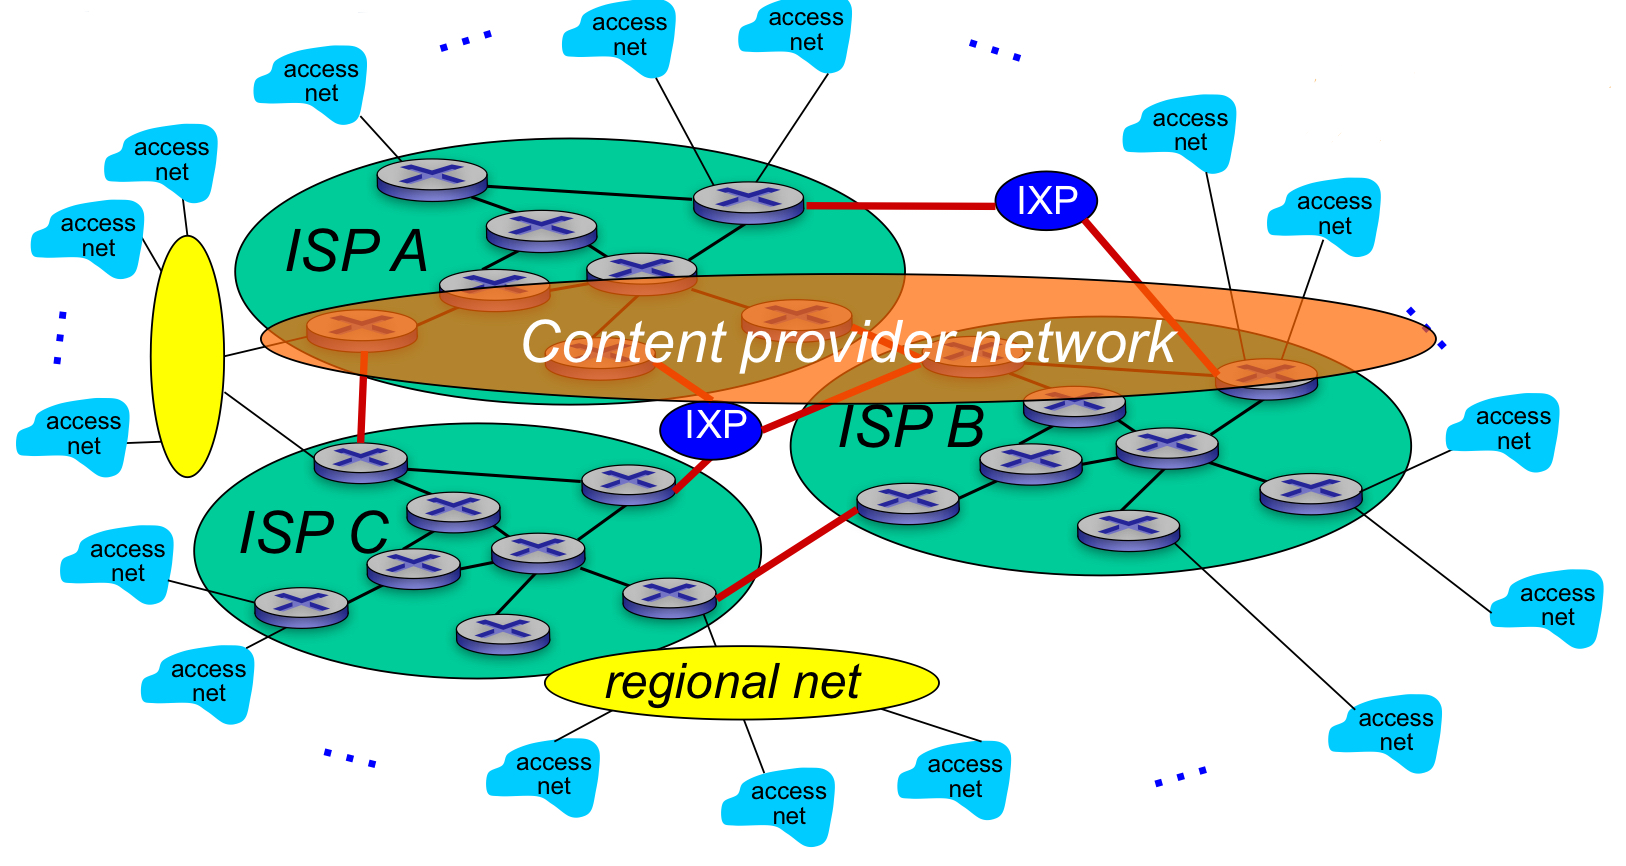
\includegraphics[scale=0.15]{internet}

\begin{itemize}
    \item End systems connect to Internet via \textbf{Access Internet Service Providers (ISPs)}
    \item ISPs connect to larger global ISPs (usually competitors)
    \item Large ISPs connect via \textbf{peering links} or \textbf{internet exchange points (IXP)}
    \item \keyword{IXP}{Physical place with routers from different ISPs}
    \item \keyword{Regional Networks}{Smallers ISPs}
    \item \keyword{Content Provider Networks}{Provide content close to end users}
\end{itemize}

\subsection{Loss, Delay, and Throughput}

\subsubsection{Packet Loss}

\begin{itemize}
    \item If Arrival Rate $>$ Transmission Rate, packets will queue and can be dropped if queue fills up
    \item Solutions: Lost packets can be retransmitted
\end{itemize}

\subsubsection{Packet Delay}

\[d_{\text{nodal}} = d_{\text{proc}} + d_{\text{queue}} + d_{\text{trans}} + d_{\text{prop}}\]

\begin{itemize}
    \item \keyword{Nodal Processing}{($d_{\text{proc}}$) Check for bit errors and determine output link}
    \item \keyword{Queueing Delay}{($d_{\text{queue}}$) Time at queue waiting for transmission}
    \item \keyword{Transmission Delay}{($d_{\text{trans}}$) Time to load packet onto link}
    \begin{itemize}
        \item $d_{\text{trans}} = \frac{L}{R}$ where $L$ is packet length and $R$ is link bandwidth
    \end{itemize}
    \item \keyword{Propagation Delay}{($d_{\text{prop}}$) Time for 1 bit to reach end of link}
    \begin{itemize}
        \item $d_{\text{prop}} = \frac{d}{s}$ where $d$ is length of link and $s$ is propagation speed
    \end{itemize}
\end{itemize}

\subsubsection{Throughput}

\begin{itemize}
    \item Rate at which bits transferred between hosts
    \begin{itemize}
        \item Different from transmission rate, which is the theoretical upper bound
    \end{itemize}
    \item Average: Rate over long period of time
    \item Instantaneous: Rate at given point in time
\end{itemize}

\subsection{Protocol Layers and Service Models}

\begin{itemize}
    \item \keyword{Protocol}{Defines format, order of messages sent and received, and actions taken on message transmission}
    \item Networks are complex with many components. How can we organize its structure?
    \item \keyword{Layering}{Each layer implements a service by doing something within layer and relying on services provided by layer below it}
    \begin{itemize}
        \item Explicit structure allows us to make sense of complex components
        \item Easy maintenance (Like OOP, change in 1 layer should not affect others)
    \end{itemize}
\end{itemize}

\subsubsection{Internet Protocol Stack}

\begin{enumerate}
    \item Application
    \item Transport
    \item Network
    \item Link
    \item Physical
\end{enumerate}

\section{02. Application Layer}

\begin{itemize}
    \item Programs that run on end systems, and not on network-core devices
\end{itemize}

\subsection{Client-server Architecture}

\begin{itemize}
    \item Server: Always-on host, Permanent IP address
    \item Clients: Communicates with server, Intermittently connected, Dynamic IP addresses, Do not communicate with each other directly
\end{itemize}

\subsection{P2P Architecture}

\begin{itemize}
    \item Peers request service from other peers and provide service in return
    \item No always-on server, Intermittently connected, Dynamic IP addresses
    \item \keyword{Self Scalability}{New peers offer new services and demands}
\end{itemize}

\subsection{Process}

\begin{itemize}
    \item \keyword{Process}{Program running in host}
    \item \keyword{Inter-process Communication}{How 2 processes in 1 host communicate}
    \item \keyword{Messages}{Processes in different hosts communicate by exchanging this}
    \item \keyword{Client Process}{Process that initiates communication}
    \item \keyword{Server Process}{Process that waits to be contacted}
    \item \keyword{Socket}{Process sends/receives messages to/from its socket (like a door)}
    \begin{itemize}
        \item Outside of socket, transport layer delivers message
    \end{itemize}
\end{itemize}

\subsection{Addressing Processes}

\begin{itemize}
    \item Motivation: IP address is not enough to address process, since many processes can be running on same host
    \begin{itemize}
        \item \keyword{Identifier}{IP address and port number}
        \item \keyword{Port Number:}{Associated with process on host}
    \end{itemize}
\end{itemize}

\subsection{Transport Protocol Services}

\begin{enumerate}
    \item \keyword{TCP}{Transmission Control Protocol}
    \begin{itemize}
        \item Reliable transport
        \item Flow control: Sender does not overwhelm receiver
        \item Congestion control
        \item Connection-oriented: Setup required between client and server
    \end{itemize}
    \item \keyword{UDP}{User Datagram Protocol}
    \begin{itemize}
        \item Unreliable data transfer
        \item Fast
    \end{itemize}
\end{enumerate}

\subsection{App-layer Protocol}

\begin{itemize}
    \item Types of messages exchanged (e.g. Request or response)
    \item Message syntax: How fields are delineated
    \item Messages semantics: Meaning of information in fields
\end{itemize}

\subsection{HTTP}

\begin{itemize}
    \item \keyword{Hypertext Transfer Protocol}{Web's application layer protocol}
    \item Motivation: Web page consists of objects (HTML, images). Need method to request/send web objects.
    \item Follows client/server model
    \item Uses TCP
    \item \keyword{Stateless}{Server maintains no information about past requests}
\end{itemize}

\subsubsection{Non-persistent HTTP}

\begin{itemize}
    \item At most 1 object sent over TCP connection
    \item Downloading multiple objects requires multiple TCP connections
\end{itemize}

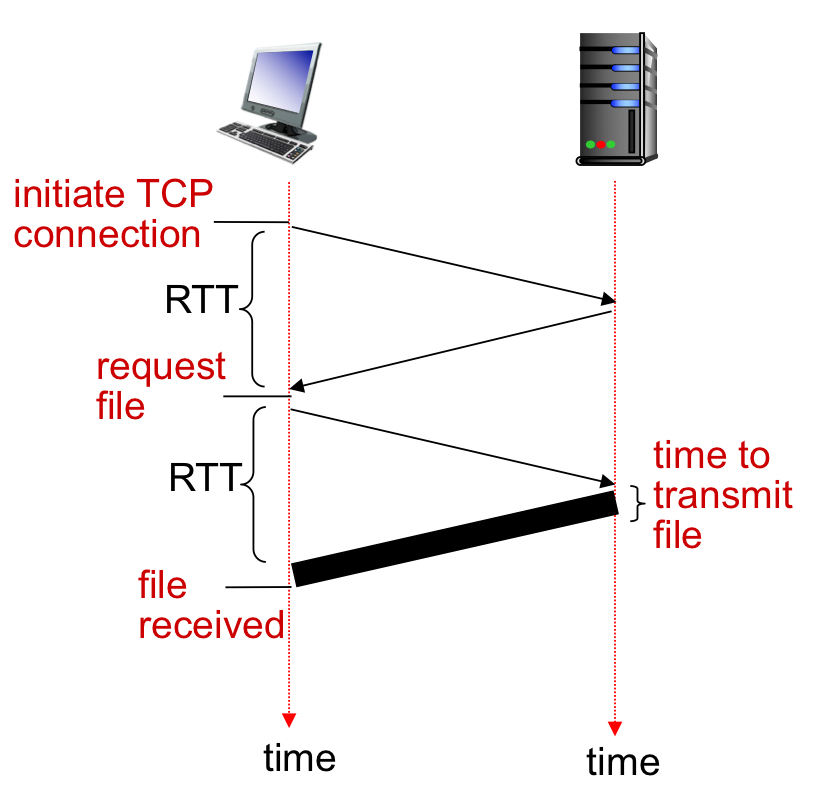
\includegraphics[scale=0.15]{non-persistent-http}

\begin{itemize}
    \item Server closes TCP connection after sending file
    \item \keyword{Return Trip Time}{(RTT) Time for small packet to travel from client to server and back}
    \item Response Time: 2 RTT + File transmission time
\end{itemize}

\subsubsection{Persistent HTTP}

\begin{itemize}
    \item Multiple objects can be sent over single TCP connection
    \item Server leaves TCP connection open after sending response
    \item Subsequent objects can use same TCP connection and be sent using 1 RTT + File transmission time
\end{itemize}

\subsubsection{HTTP Request Message}

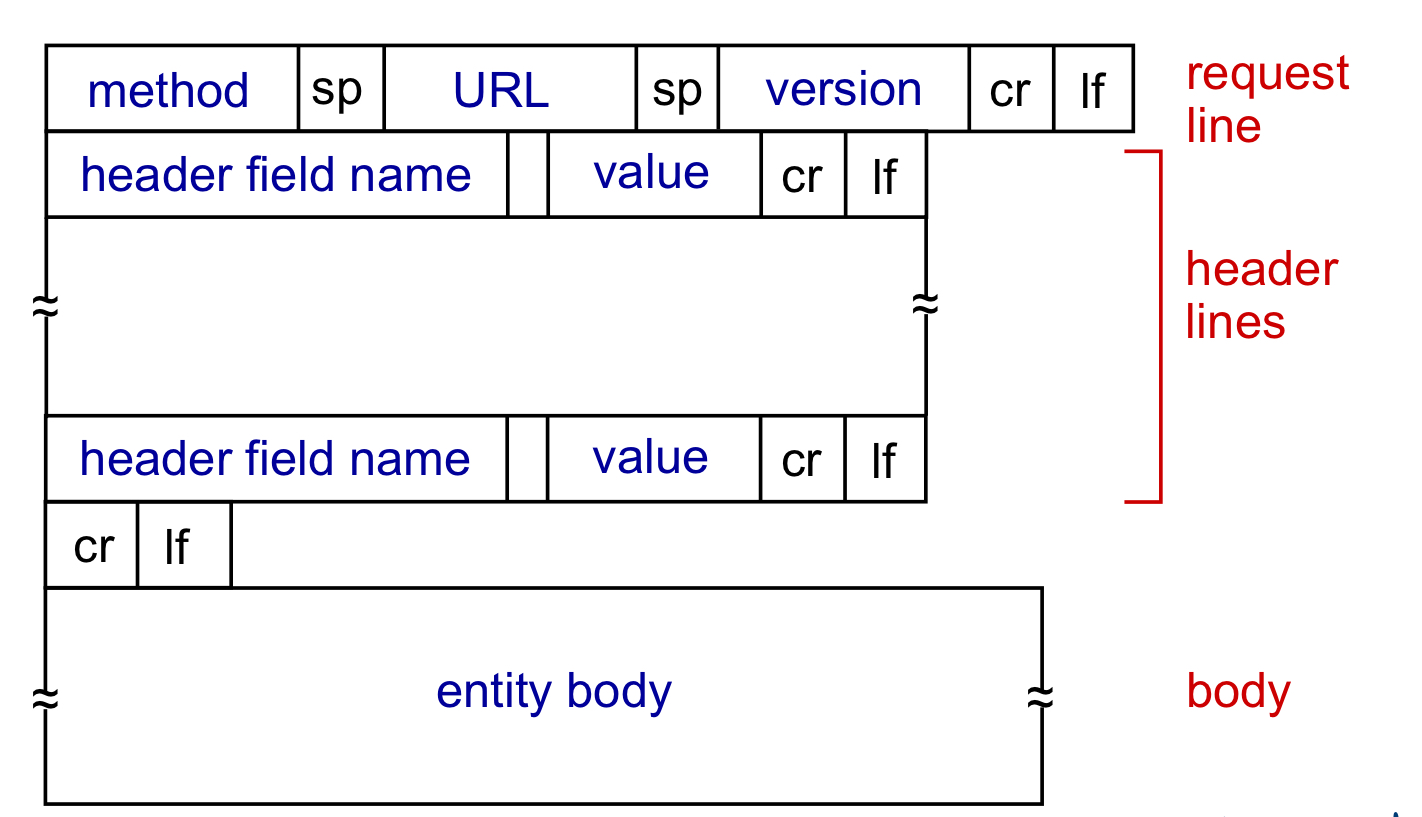
\includegraphics[scale=0.12]{http-request}

\begin{itemize}
    \item To upload form input: \keyword{POST method}{Input uploaded via entity body} and \keyword{URL method}{Input uploaded in URL field of GET method}
    \item \keyword{HTTP/1.0}{GET, POST, HEAD (Ask server to leave request object out of response). Non-persistent by default.}
    \item \keyword{HTTP/1.1}{GET, POST, HEAD, PUT, DELETE. Persistent by default.}
\end{itemize}

\subsubsection{HTTP Response Message}

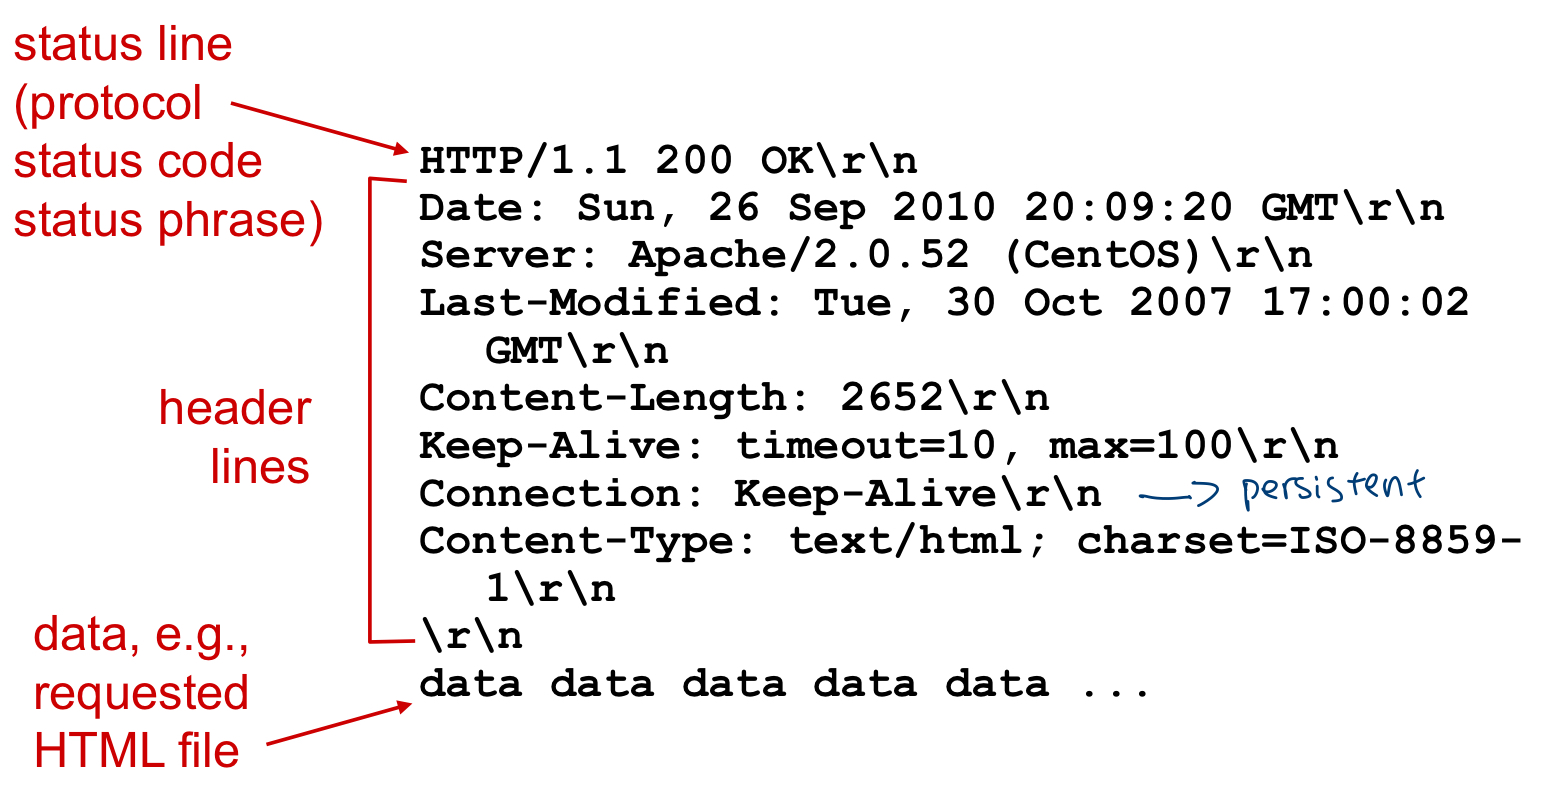
\includegraphics[scale=0.15]{http-response}

\subsubsection{Cookies}

\begin{itemize}
    \item Maintains state on client side
    \item Components: Cookie header for HTTP response, Cookie header for HTTP request, Cookie file on user's host (Key-value pair), Database on server
\end{itemize}

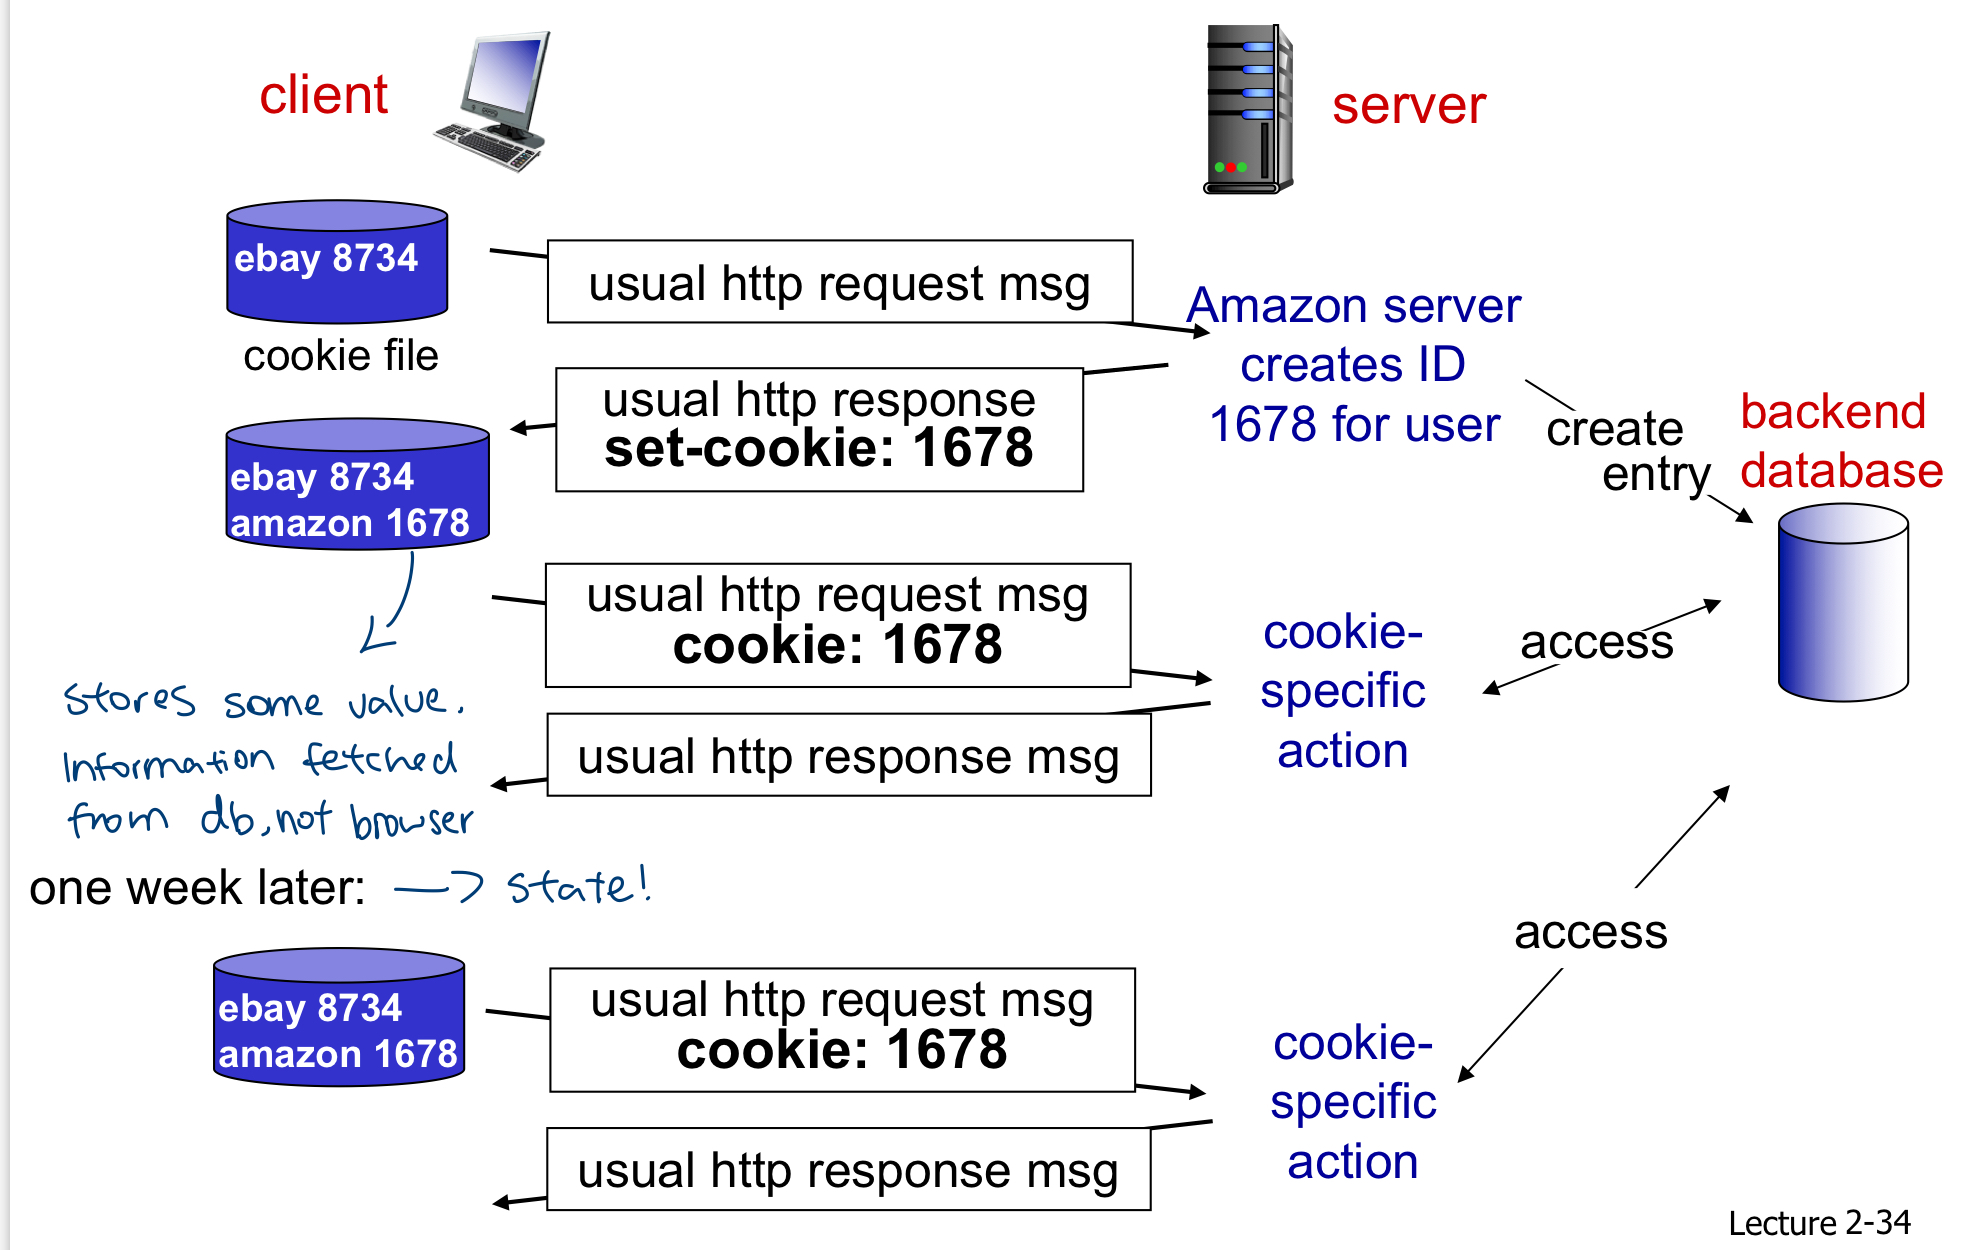
\includegraphics[scale=0.12]{cookies}

\subsubsection{Web Cache (Proxy Server)}

\begin{itemize}
    \item Goal: Fulfill request without involving origin server via caching
    \item Browser sends all HTTP requests to cache
    \item Pros: Faster, Reduces traffic to origin server
    \item Cons: What if origin server updates?
    \begin{itemize}
        \item \keyword{Conditional GET}{Origin server doesn't send object if cache has updated version}
        \item Cache: Specifies date of cached copy in HTTP request to origin
        \item Origin Server: Response contains no object if cached object is updated
    \end{itemize}
\end{itemize}

\subsection{Domain Name System}

\begin{itemize}
    \item Maps between IP address and name (e.g. yahoo.com)
    \item Implemented using distributed and hierarchical databases
    \item Application-layer protocol
    \item Uses UDP
    \item \keyword{Local DNS Name Server}{Local cache of name-to-address mapping. Forwards query into hierarchy.}
    \begin{itemize}
        \item \keyword{Time to Live}{(TTL) Cached mappings disappear after some time}
    \end{itemize}
    \item \keyword{Root Name Server}{Contacted by local name server that cannot resolve name. Provides IP address of TLD servers.}
    \item \keyword{Top-level Domain Server}{(TLD) Provides IP address of authoritative server}
    \item \keyword{Authoritative DNS Server}{Organization's own DNS server. Provides mappings for organization's named hosts.}
    \item Iterated query: "Not sure, ask this server"
\end{itemize}

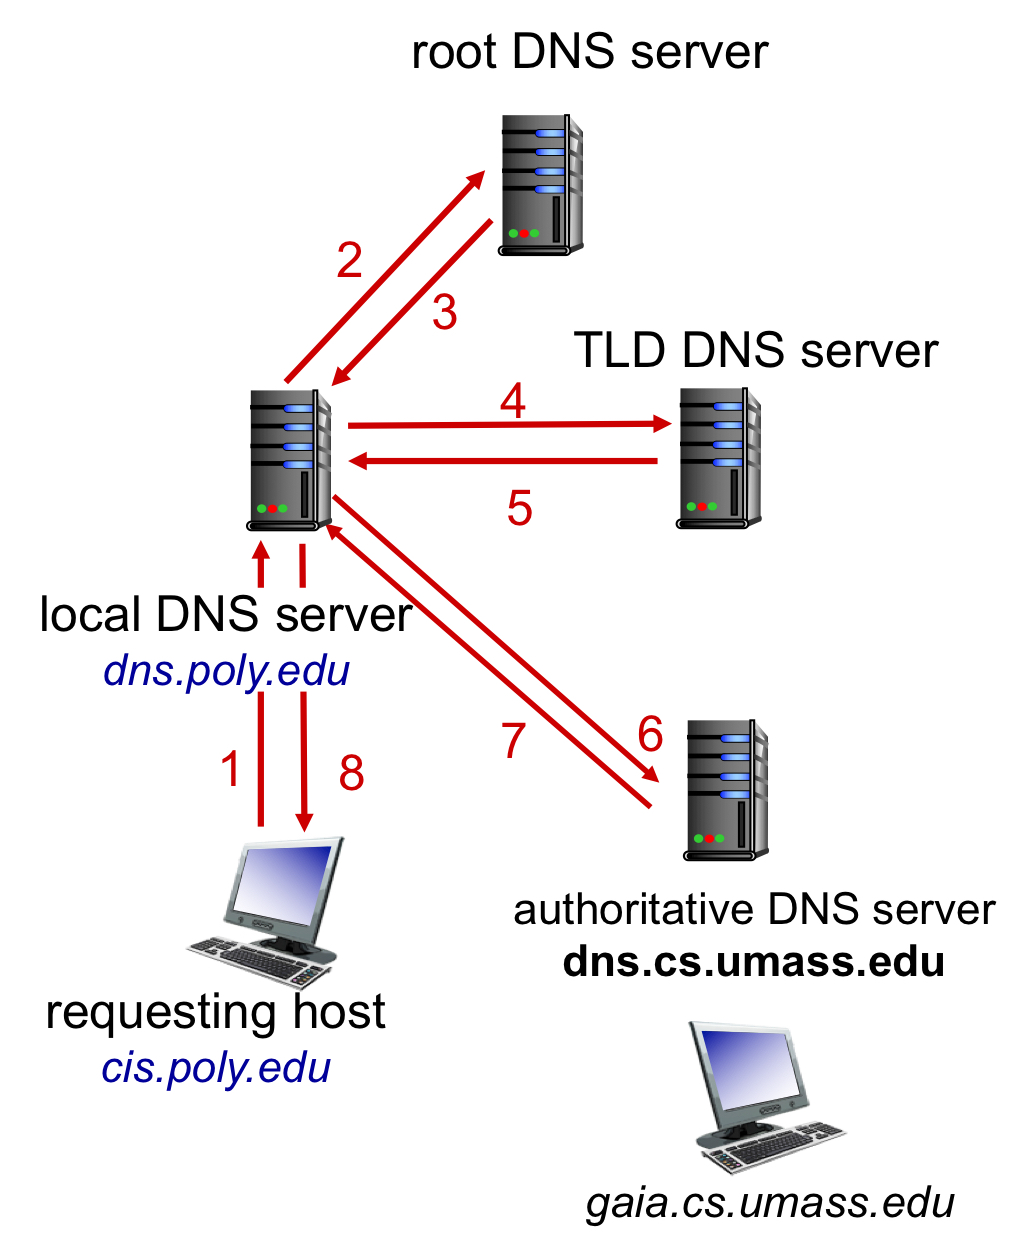
\includegraphics[scale=0.1]{dns-iterative-query}

\begin{itemize}
    \item Recursive query: "Okay, let me find for you"
    \begin{itemize}
        \item Heavy load on upper levels of hierarchy
    \end{itemize}
\end{itemize}

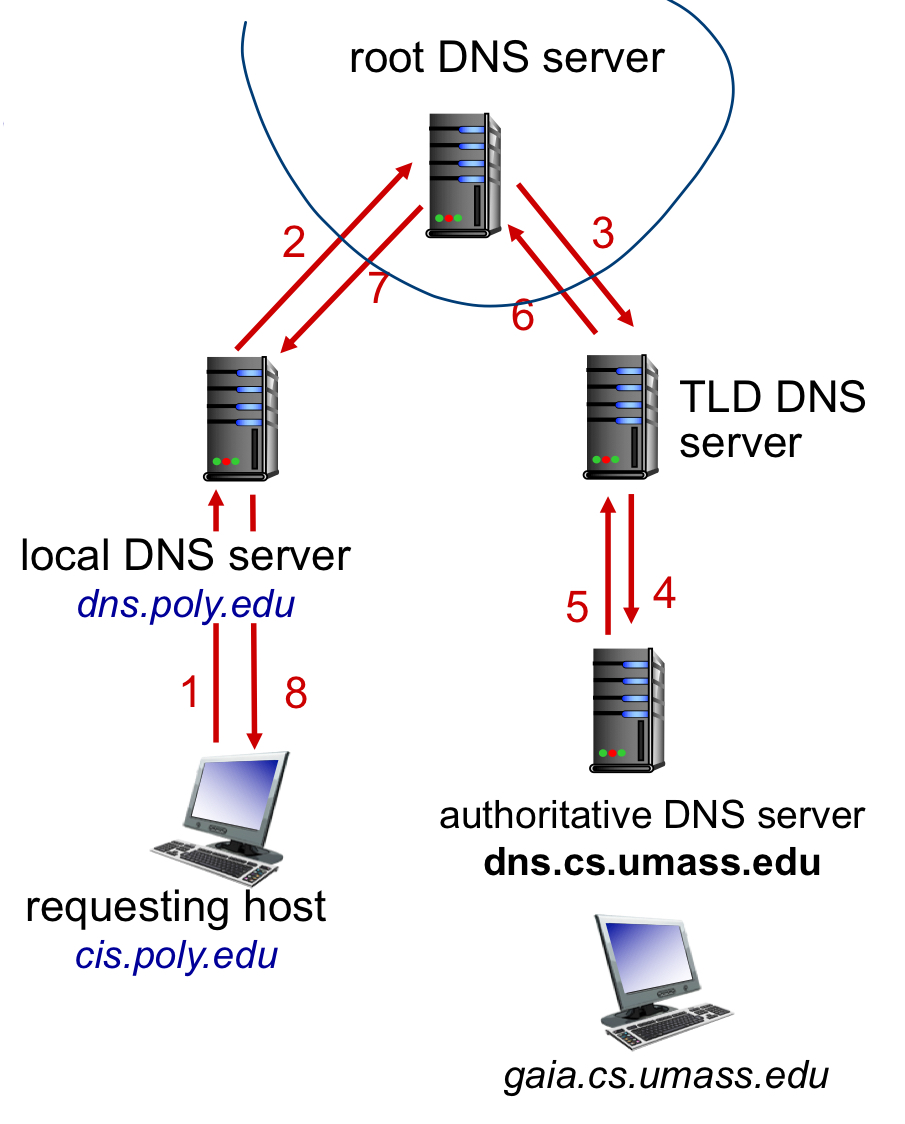
\includegraphics[scale=0.1]{dns-recursive-query}

\section{03. Socket Programming with UDP and TCP}

\subsubsection{UDP Socket}

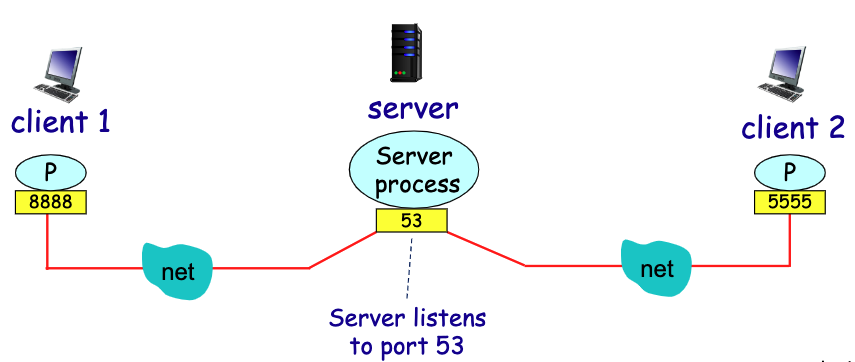
\includegraphics[scale=0.14]{udp-socket}
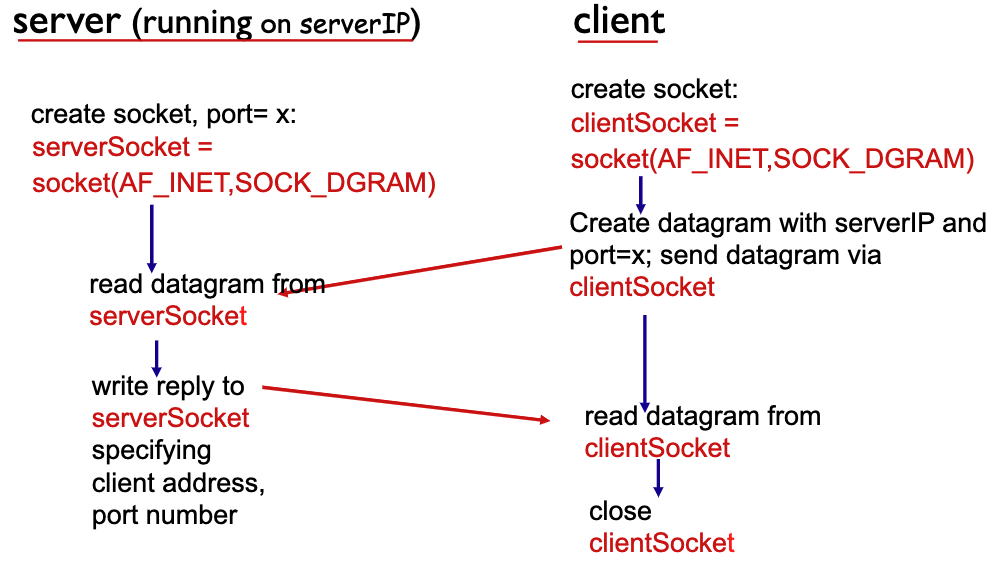
\includegraphics[scale=0.14]{udp}

\begin{itemize}
    \item No connection beforehand. Just send it.
    \item Server has 1 socket to serve all clients
    \item Sender attaches destination IP address and port number (\textbf{Stateless})
    \item Unreliable datagram: Data may be lost or out-of-order
    \begin{itemize}
        \item \keyword{Datagram}{Group of bytes}
    \end{itemize}
\end{itemize}

\subsubsection{TCP Socket}

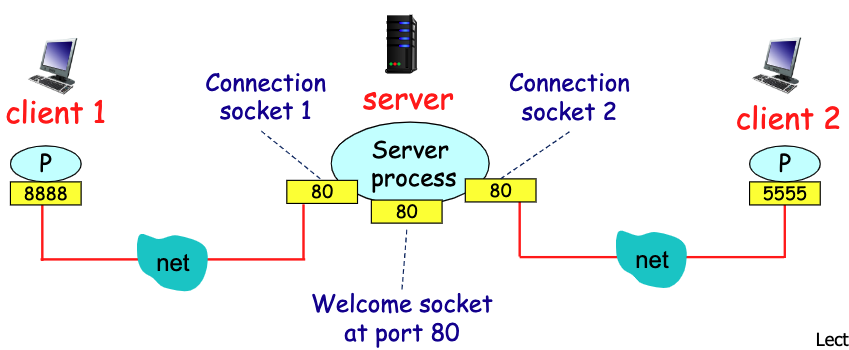
\includegraphics[scale=0.14]{tcp-socket}
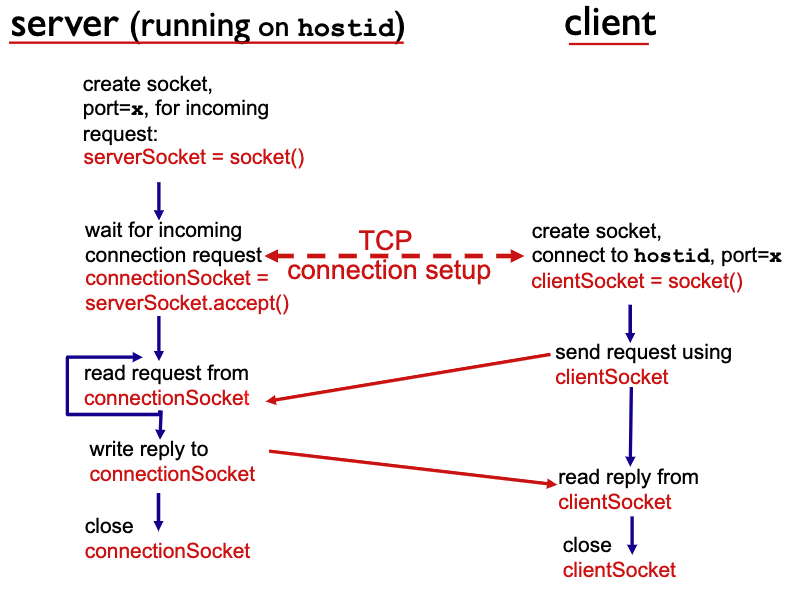
\includegraphics[scale=0.14]{tcp}

\begin{itemize}
    \item Client establishes connection to server via welcome socket
    \item Server makes new socket for each client
    \item Server identifies client via connection (\textbf{Stateful})
    \item Reliable stream pipe: Data always in order
\end{itemize}

\section{04. UDP and Reliable Protocol}

\subsection{Transport Layer Services}

\begin{itemize}
    \item Transport layer: Logical communication between \textbf{processes}
    \item Network layer: Logical communication between \textbf{hosts} (Unreliable)
\end{itemize}

\subsection{UDP}

\begin{itemize}
    \item On top of network layer, UDP adds:
    \begin{enumerate}
        \item Connectionless multiplexing/de-multiplexing
        \begin{itemize}
            \item UDP segments contain both source and destination ports
            \item Multiplexing: Sent to target processes
        \end{itemize}
        \item Checksum
    \end{enumerate}
\end{itemize}

\subsubsection{UDP Segment Header}

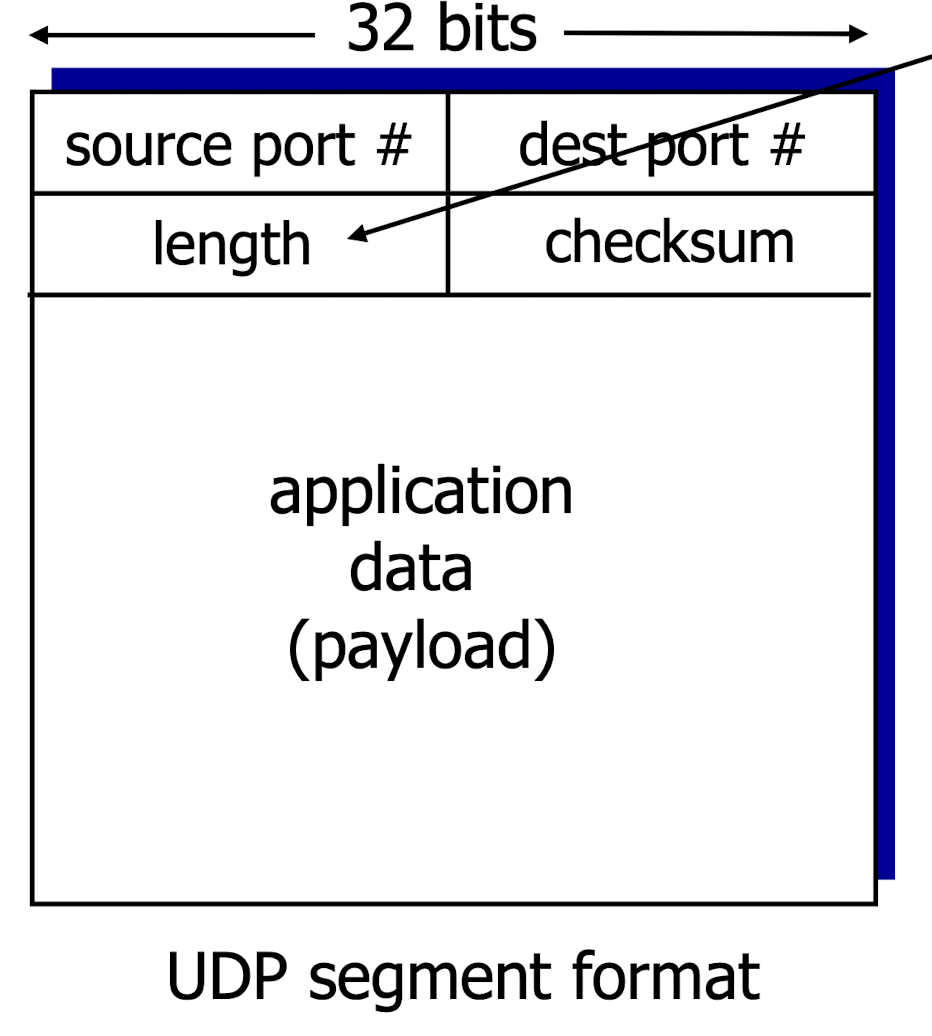
\includegraphics[scale=0.2]{udp-segment-header}

\subsubsection{Checksum}

\begin{itemize}
    \item Goal: Detect errors in received segment
\end{itemize}

\begin{enumerate}
    \item Treat UDP segment as sequence of 16-bit integers
    \item Add every 16-bit integer (Carry added back to result)
    \item Invert to get UDP checksum (1's complement)
    \item When receiving, sum segment again. All 1s if correct.
\end{enumerate}

\subsection{Reliable Data Transfer (rdt)}

\begin{itemize}
    \item Characteristics of unreliable channel will determine services provided by rdt
\end{itemize}

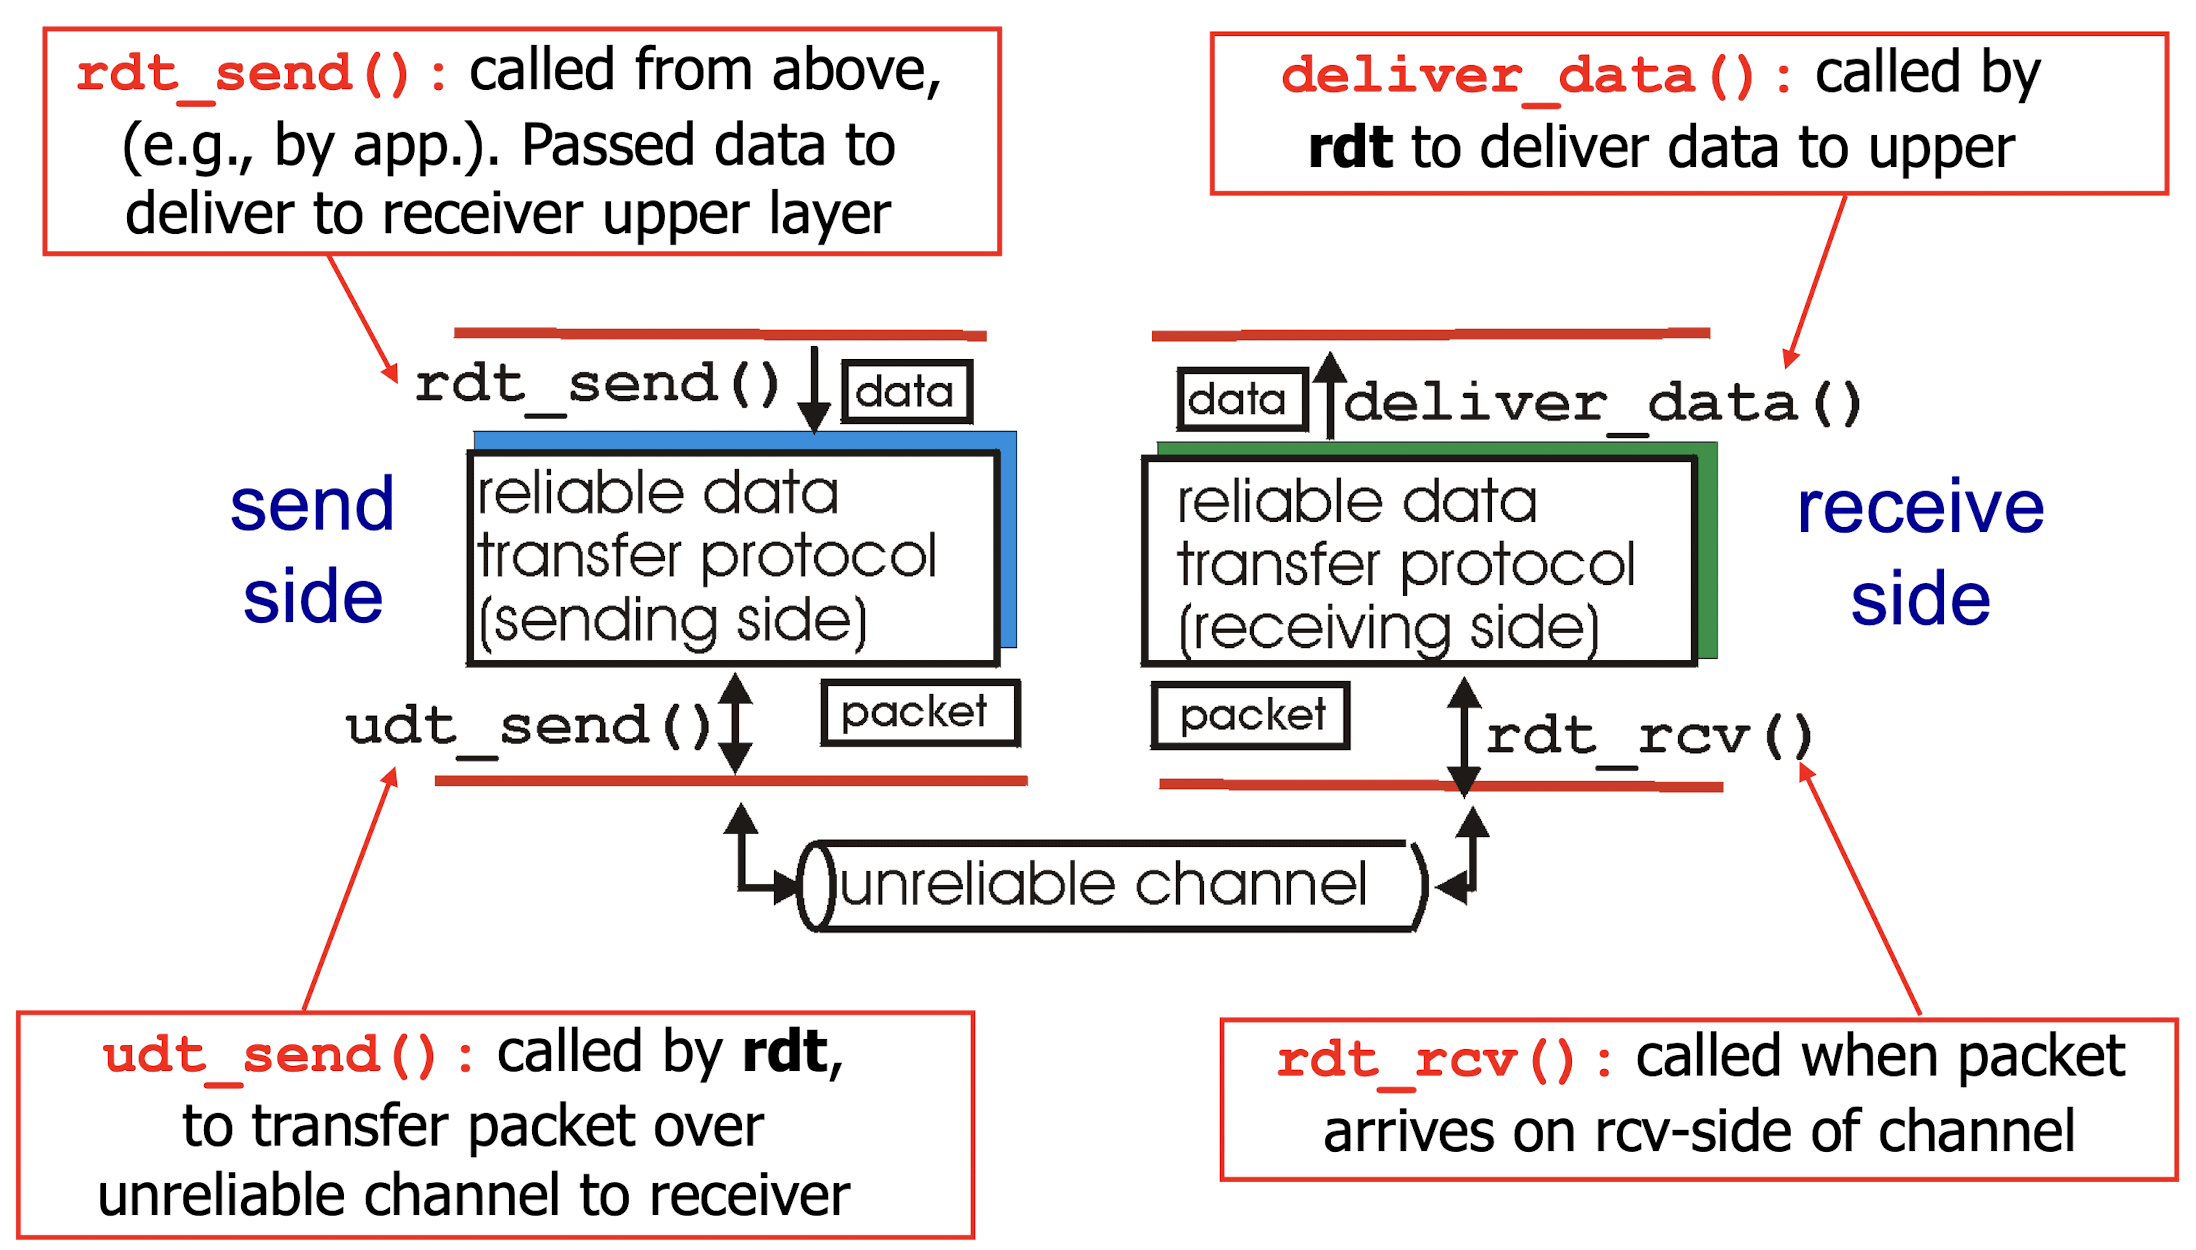
\includegraphics[scale=0.2]{rdt-interfaces}

\subsubsection{rdt 2.0}

\begin{itemize}
    \item New problem: \textbf{Bit error in data}
    \item Solution:
    \begin{itemize}
        \item Recipient perform checksum to detect bit errors
        \item \keyword{ACK}{Receiver tells sender that packet received is ok}
        \item \keyword{NAK}{Receiver tells sender that packet received has errors}
        \item After receiving NAK, sender retransmits packet 
    \end{itemize}
\end{itemize}

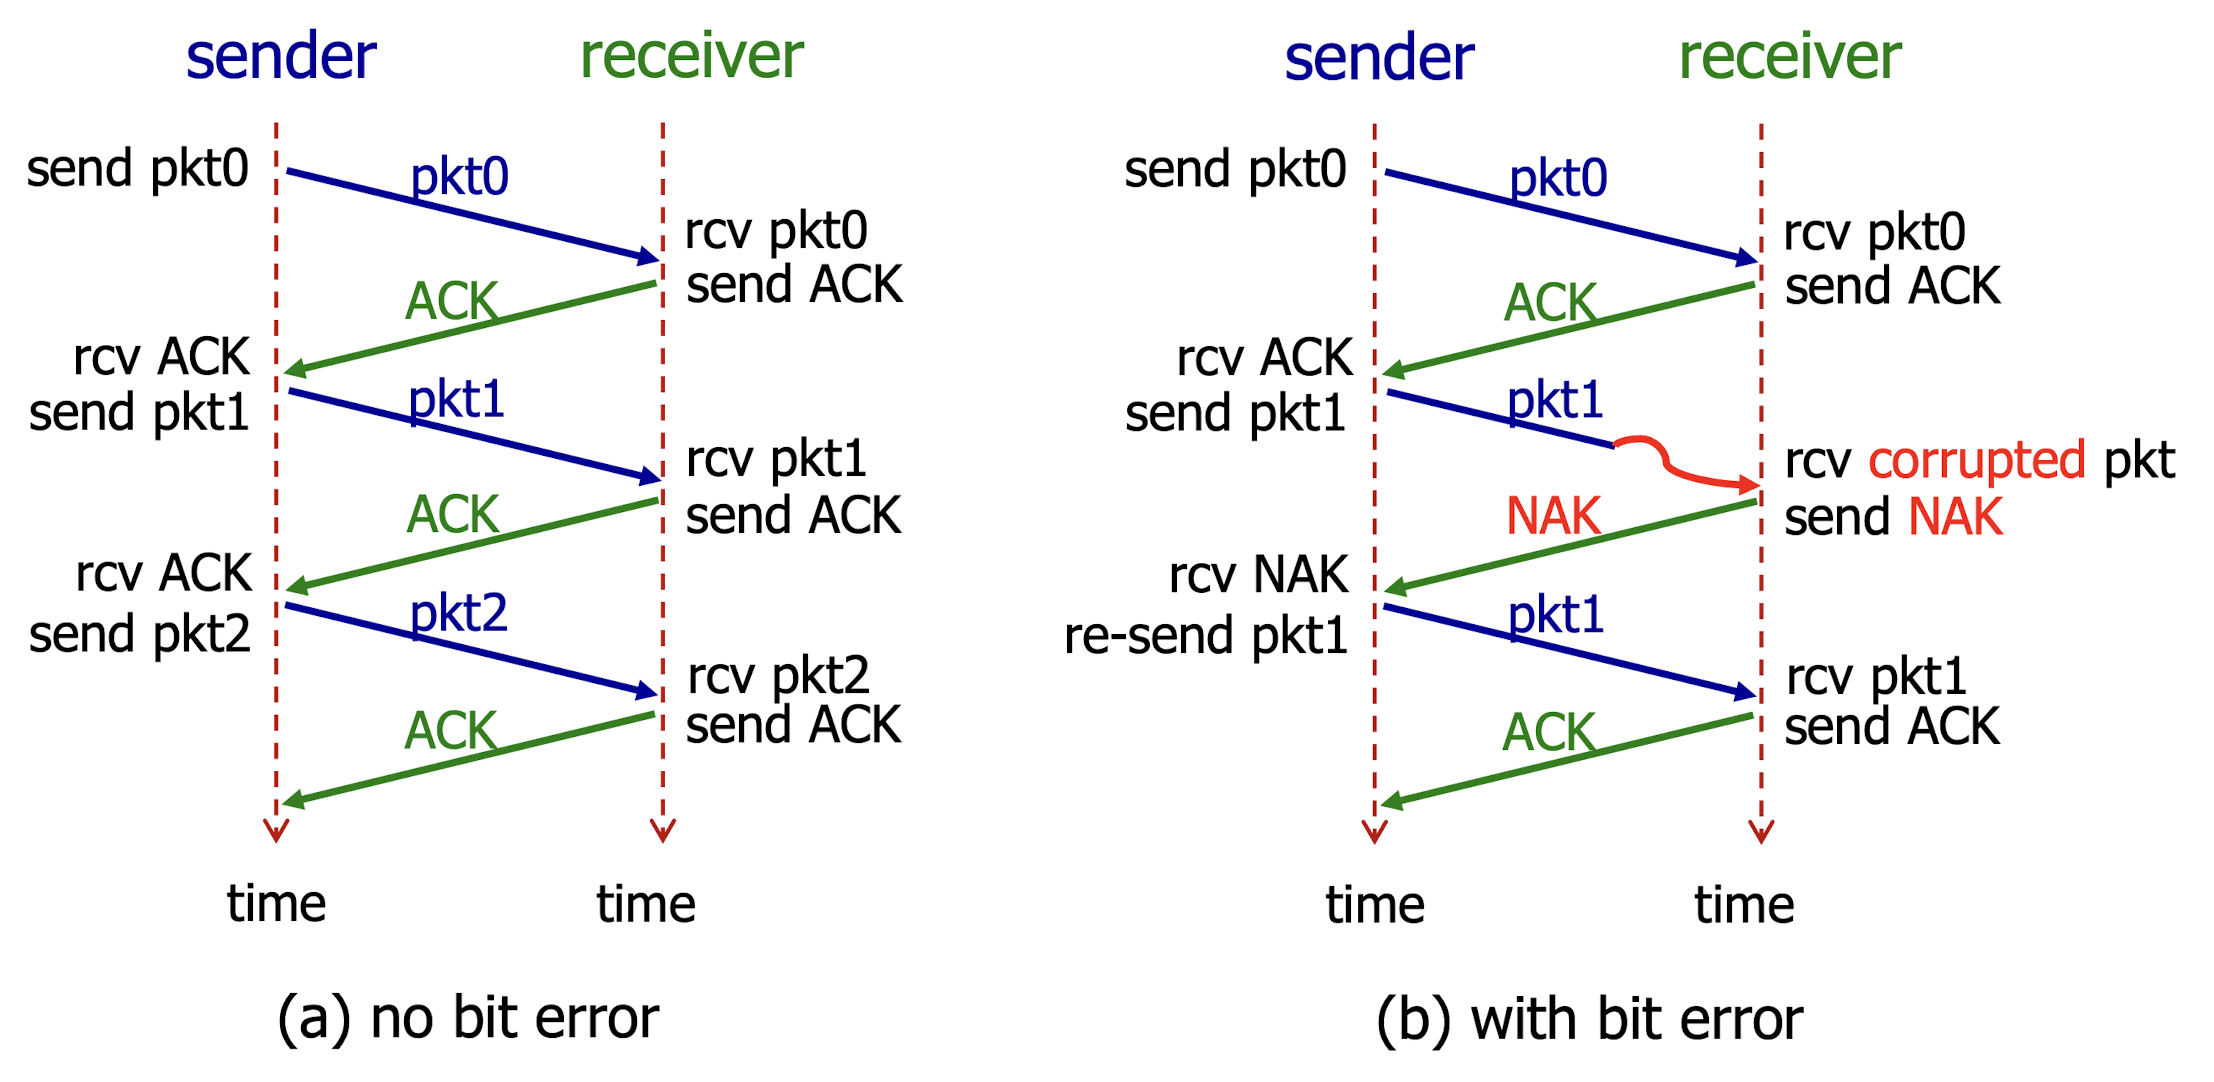
\includegraphics[scale=0.2]{rdt-2.0}

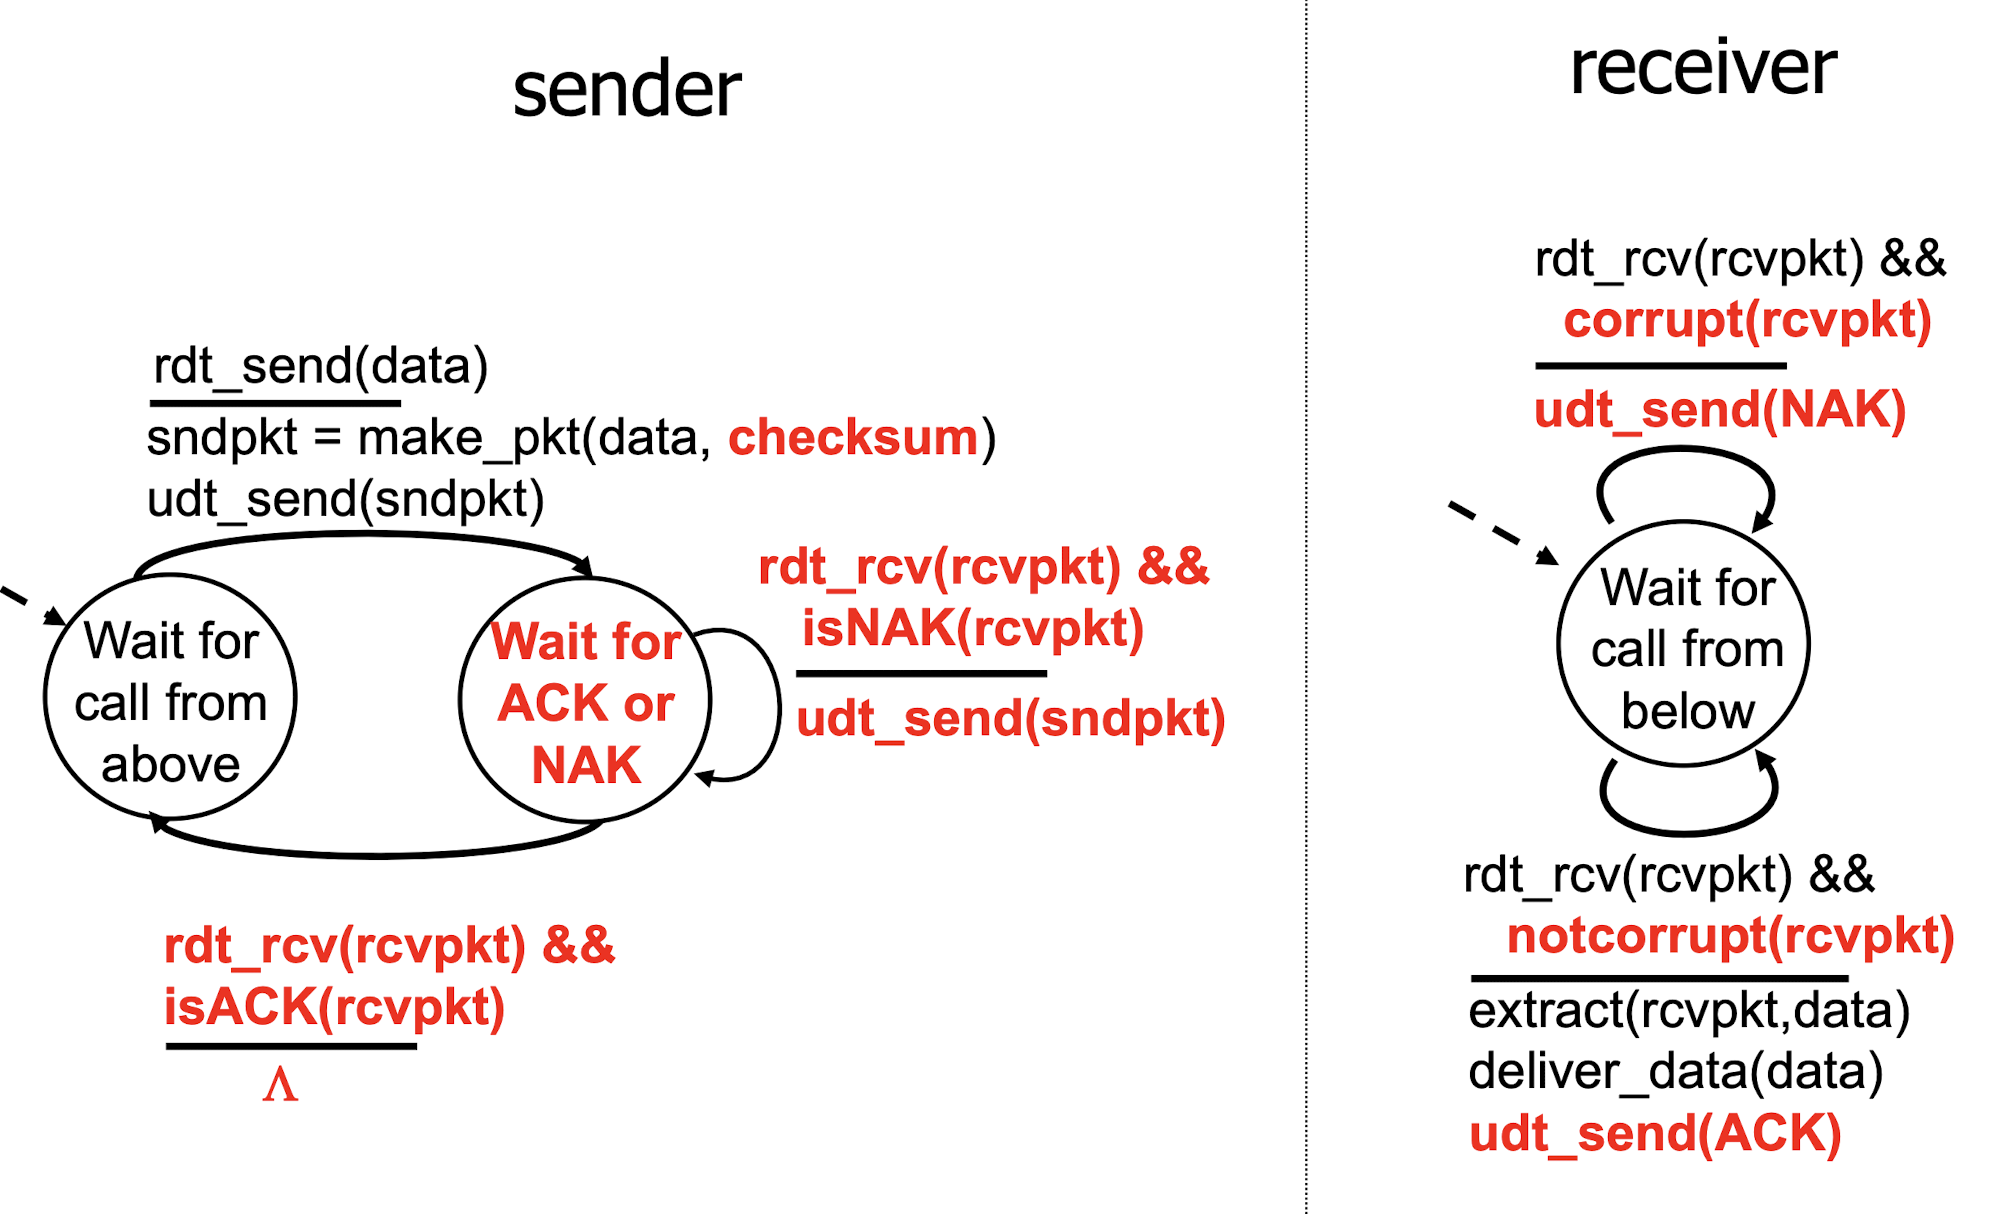
\includegraphics[scale=0.2]{rdt-2.0-fsm}

\subsubsection{rdt 2.1}

\begin{itemize}
    \item New problem: ACK/NAK may be corrupted
    \item Solution: Sender does checksum and retransmits packet if ACK/NAK is corrupted
    \item New problem: If ACK is corrupted, sender will send a \textbf{duplicate} packet
    \item Solution: Sender adds \textbf{sequence number} to each packet and receiver discards duplicate packet (Only 0 and 1 needed)
\end{itemize}

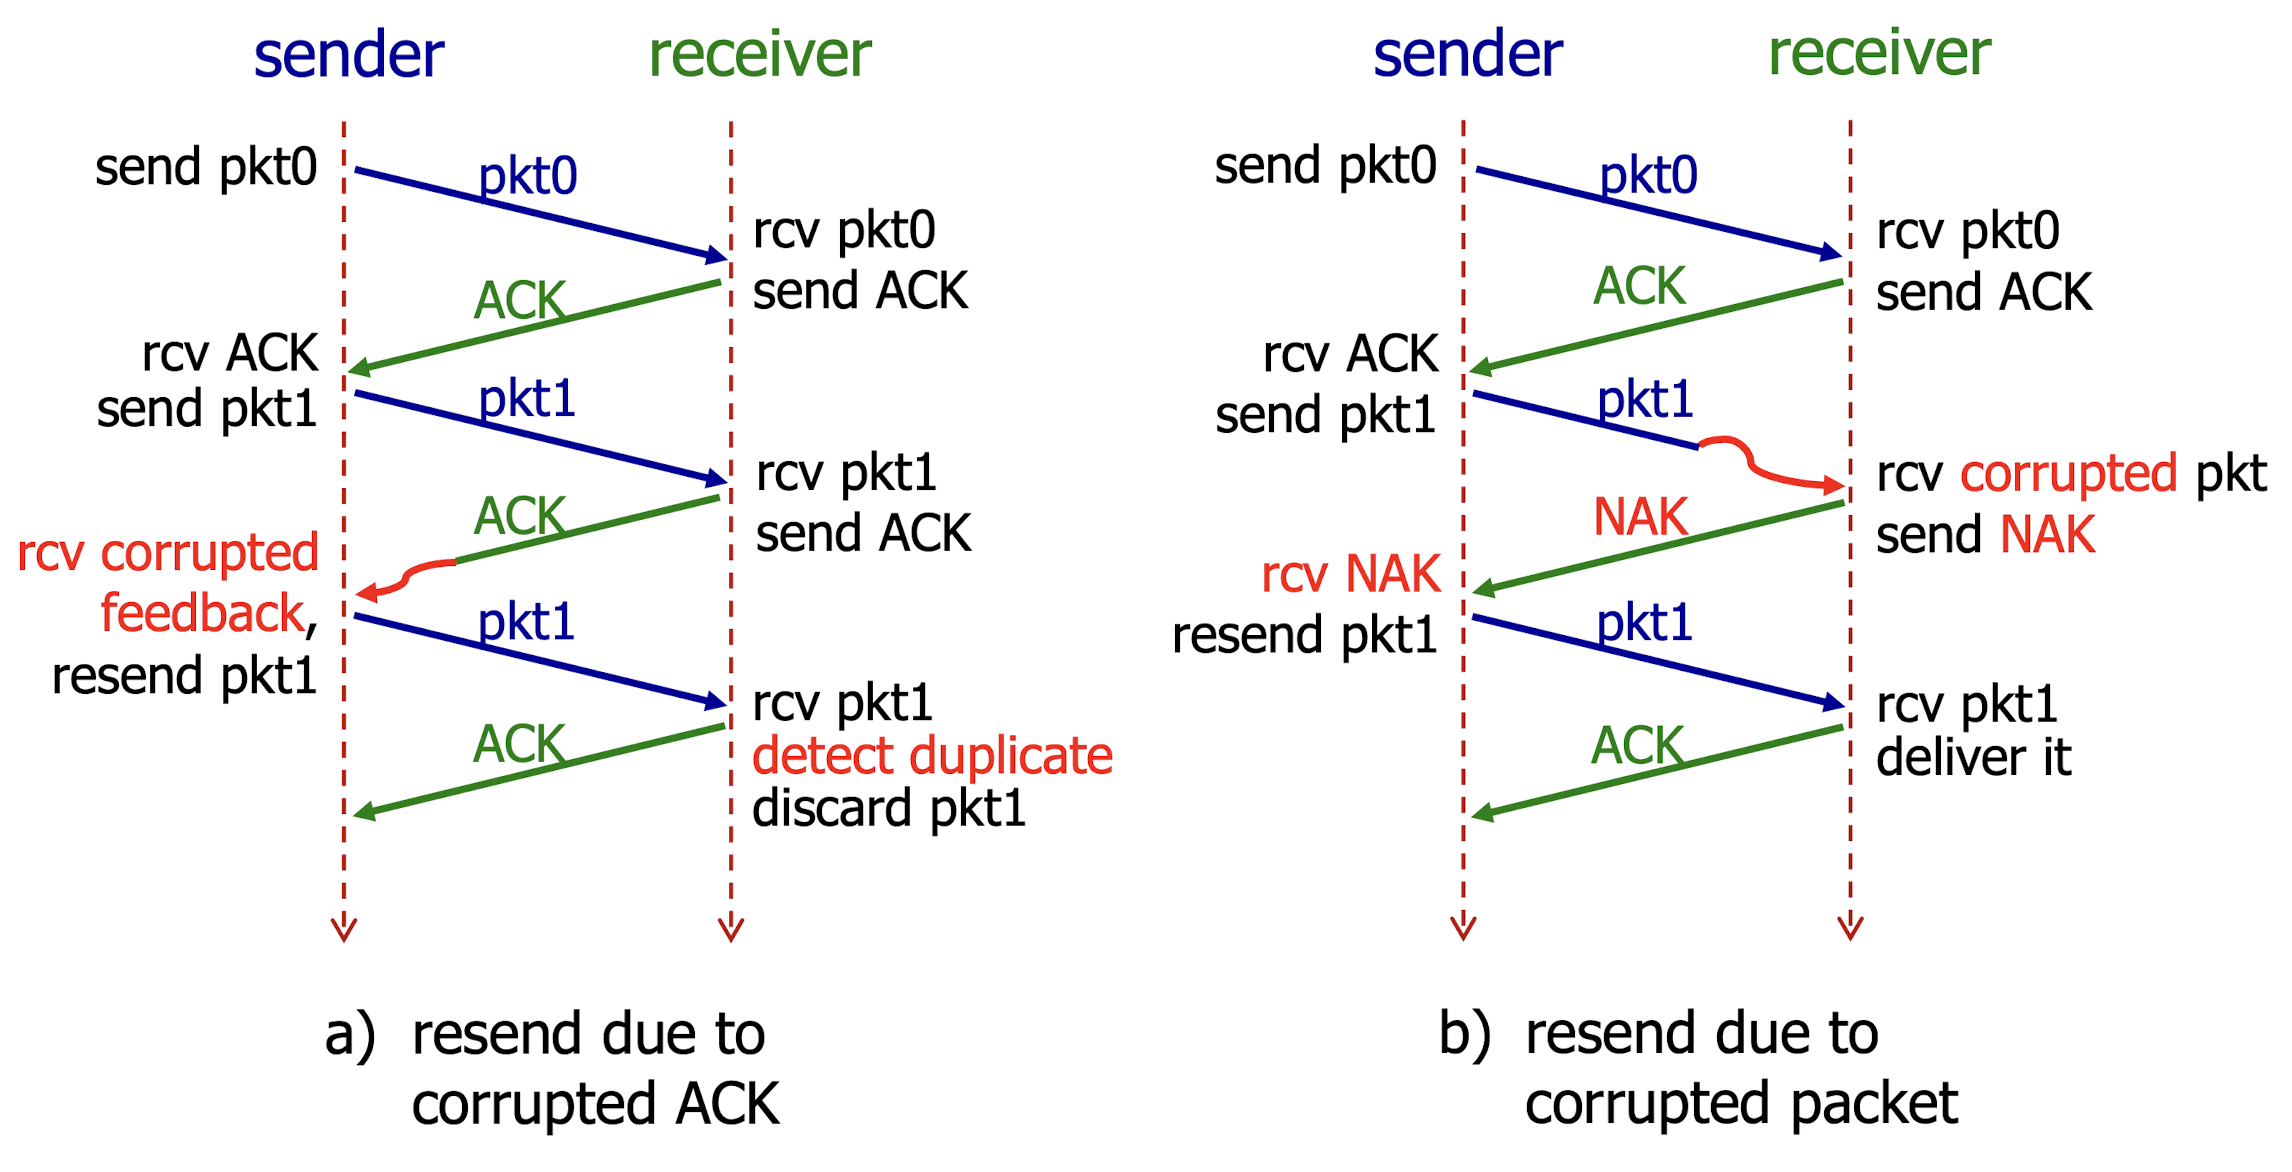
\includegraphics[scale=0.2]{rdt-2.1}

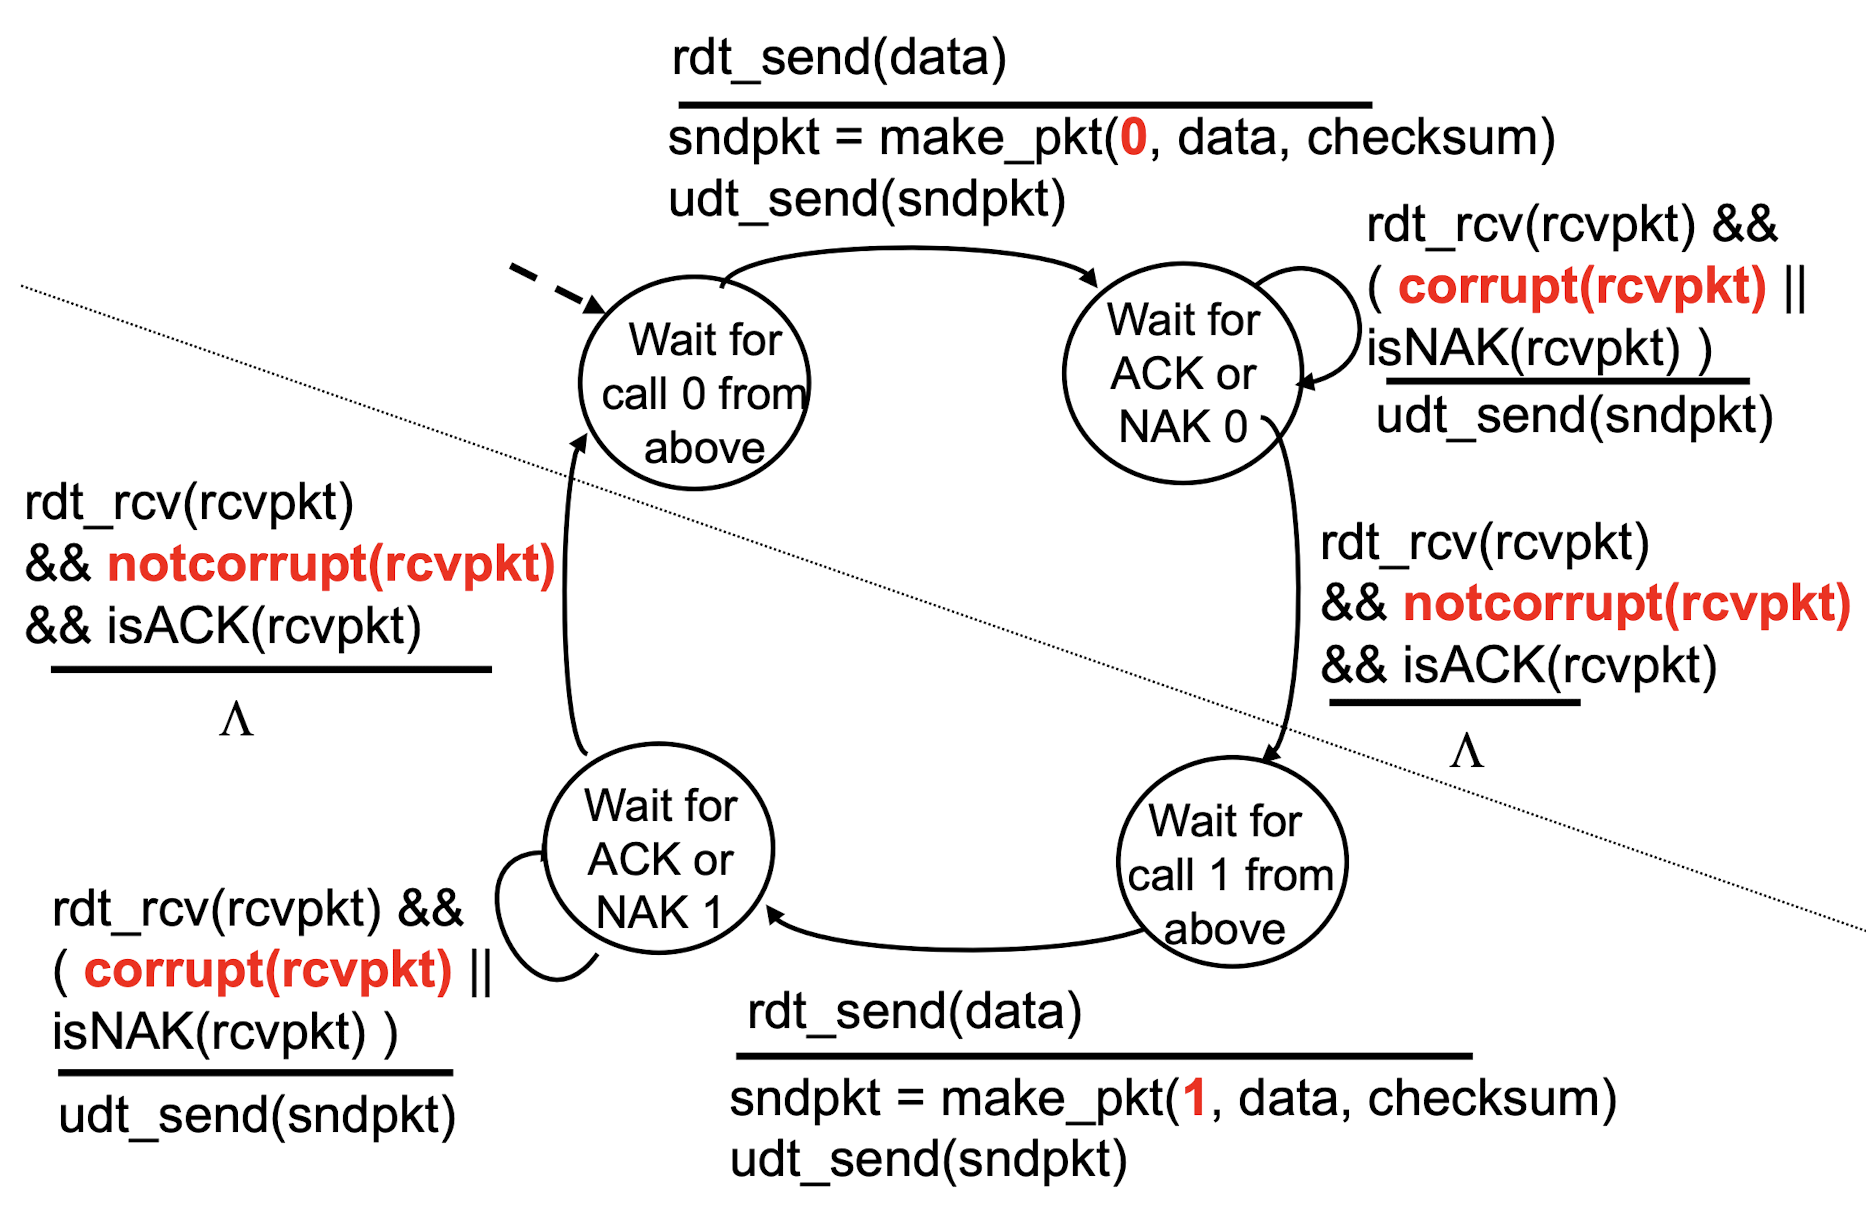
\includegraphics[scale=0.2]{rdt-2.1-sender-fsm}

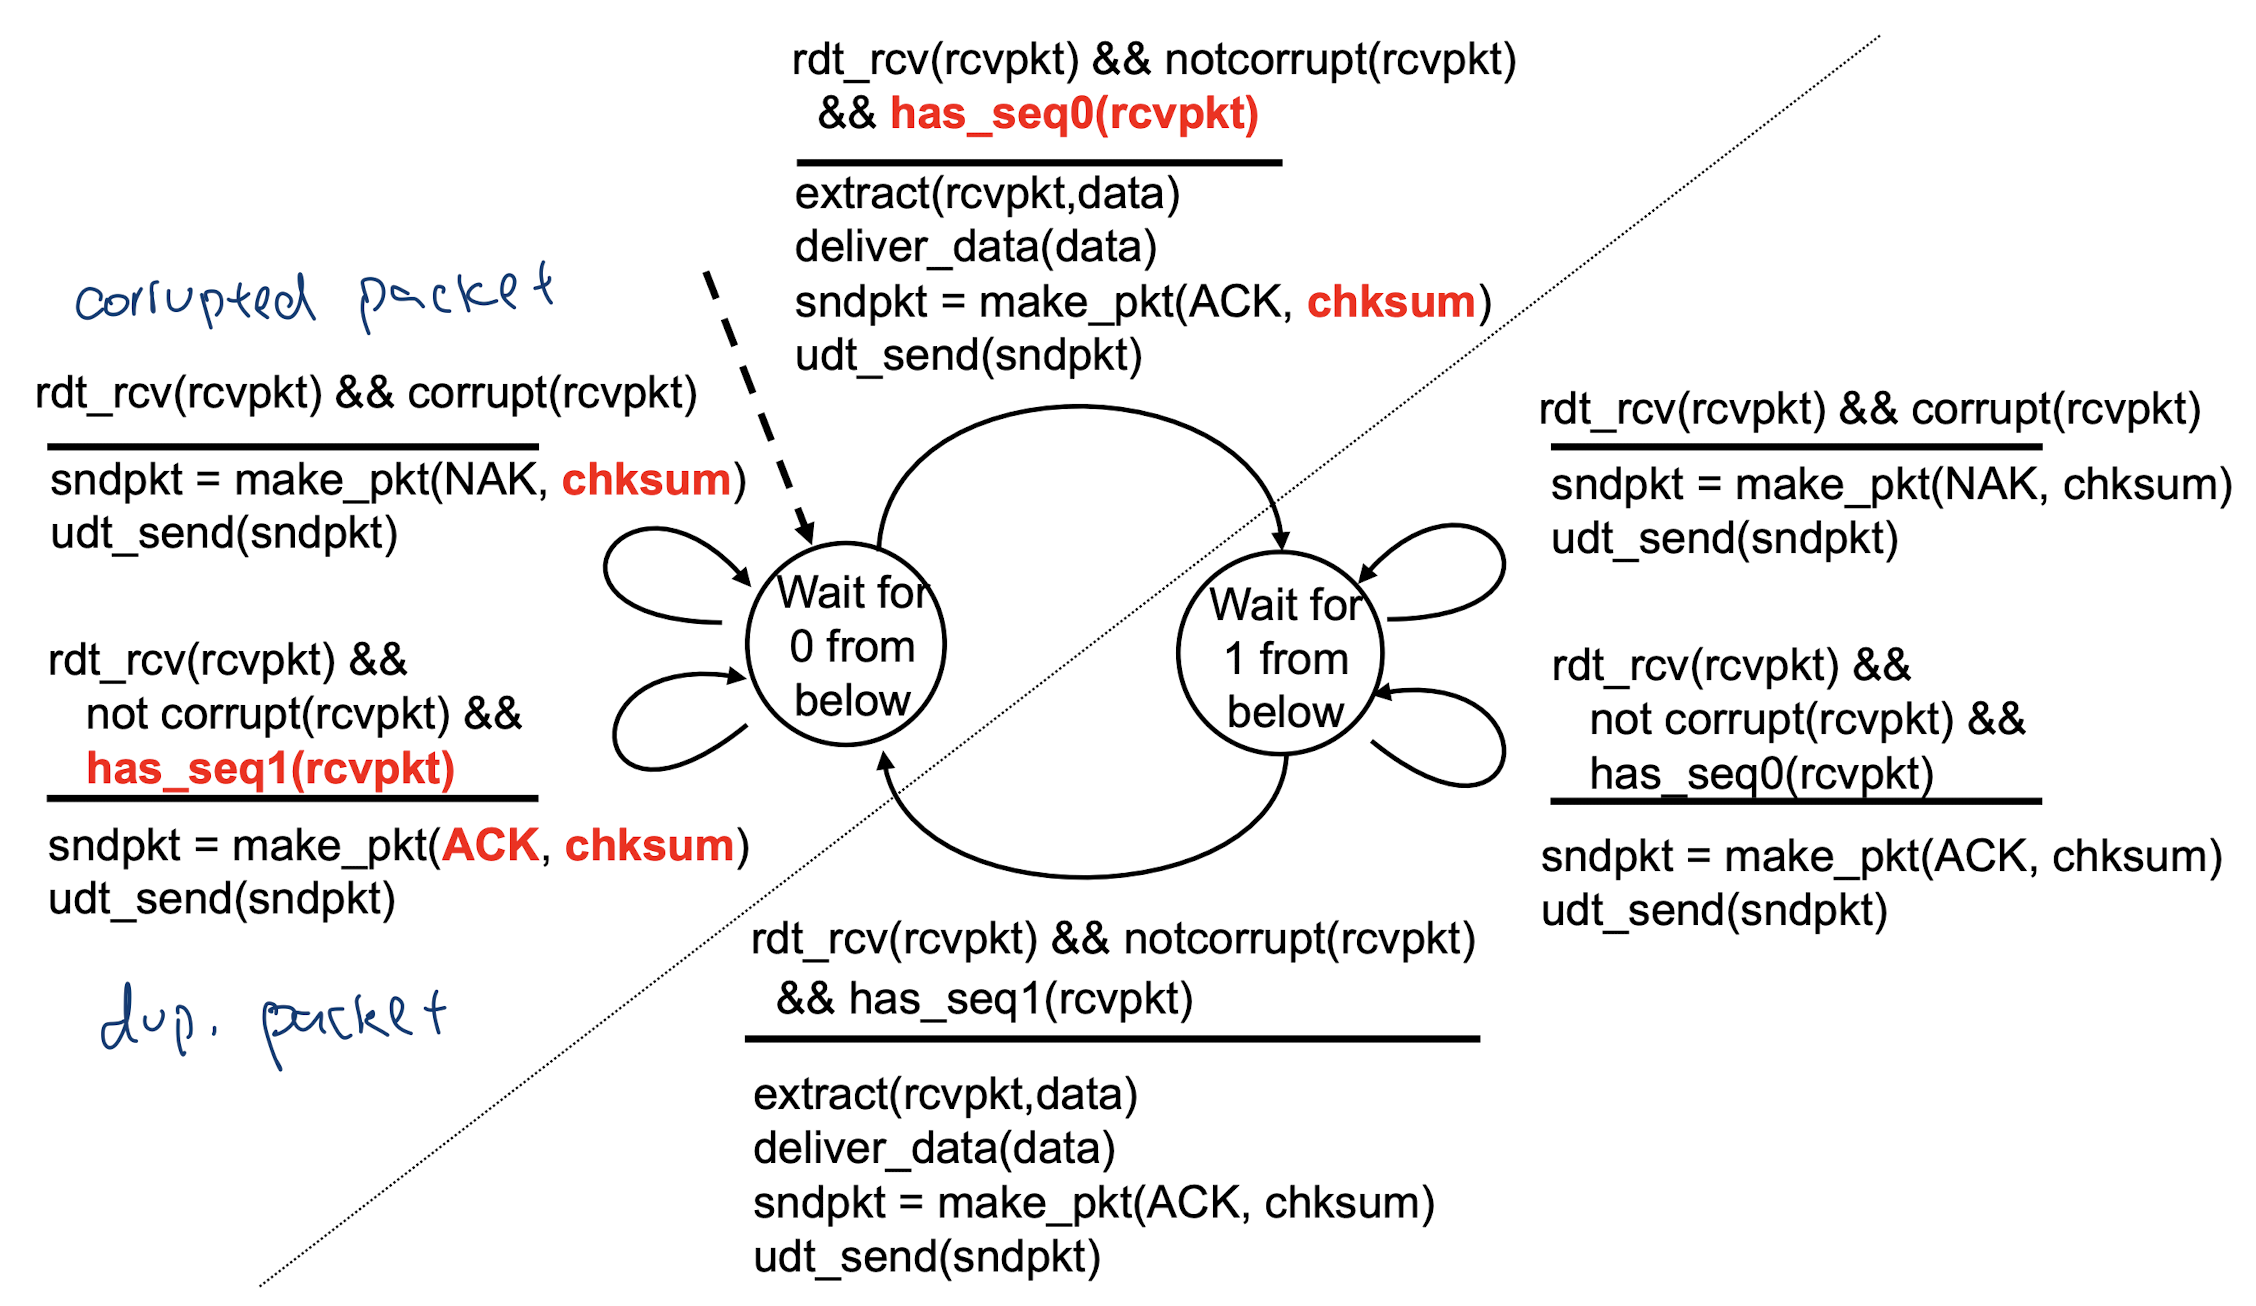
\includegraphics[scale=0.2]{rdt-2.1-receiver-fsm}

\subsubsection{rdt 2.2}

\begin{itemize}
    \item New problem: Use ACKs only. No NAK.
    \item Solution: Receiver sends ACK for last packet received. \textbf{ACK must include seq number of packet}.
\end{itemize}

\subsubsection{rdt 3.0}

\begin{itemize}
    \item New problem: Lost packets
    \item Solution: Sender waits for some time for ACK and retransmits packet
    \begin{itemize}
        \item What if duplicate packet? Sequence number handles this.
        \item What if duplicate ACK? Do nothing. Only retransmit after timeout.
        \item What if packet out of order? Have more sequence numbers.
    \end{itemize}
\end{itemize}

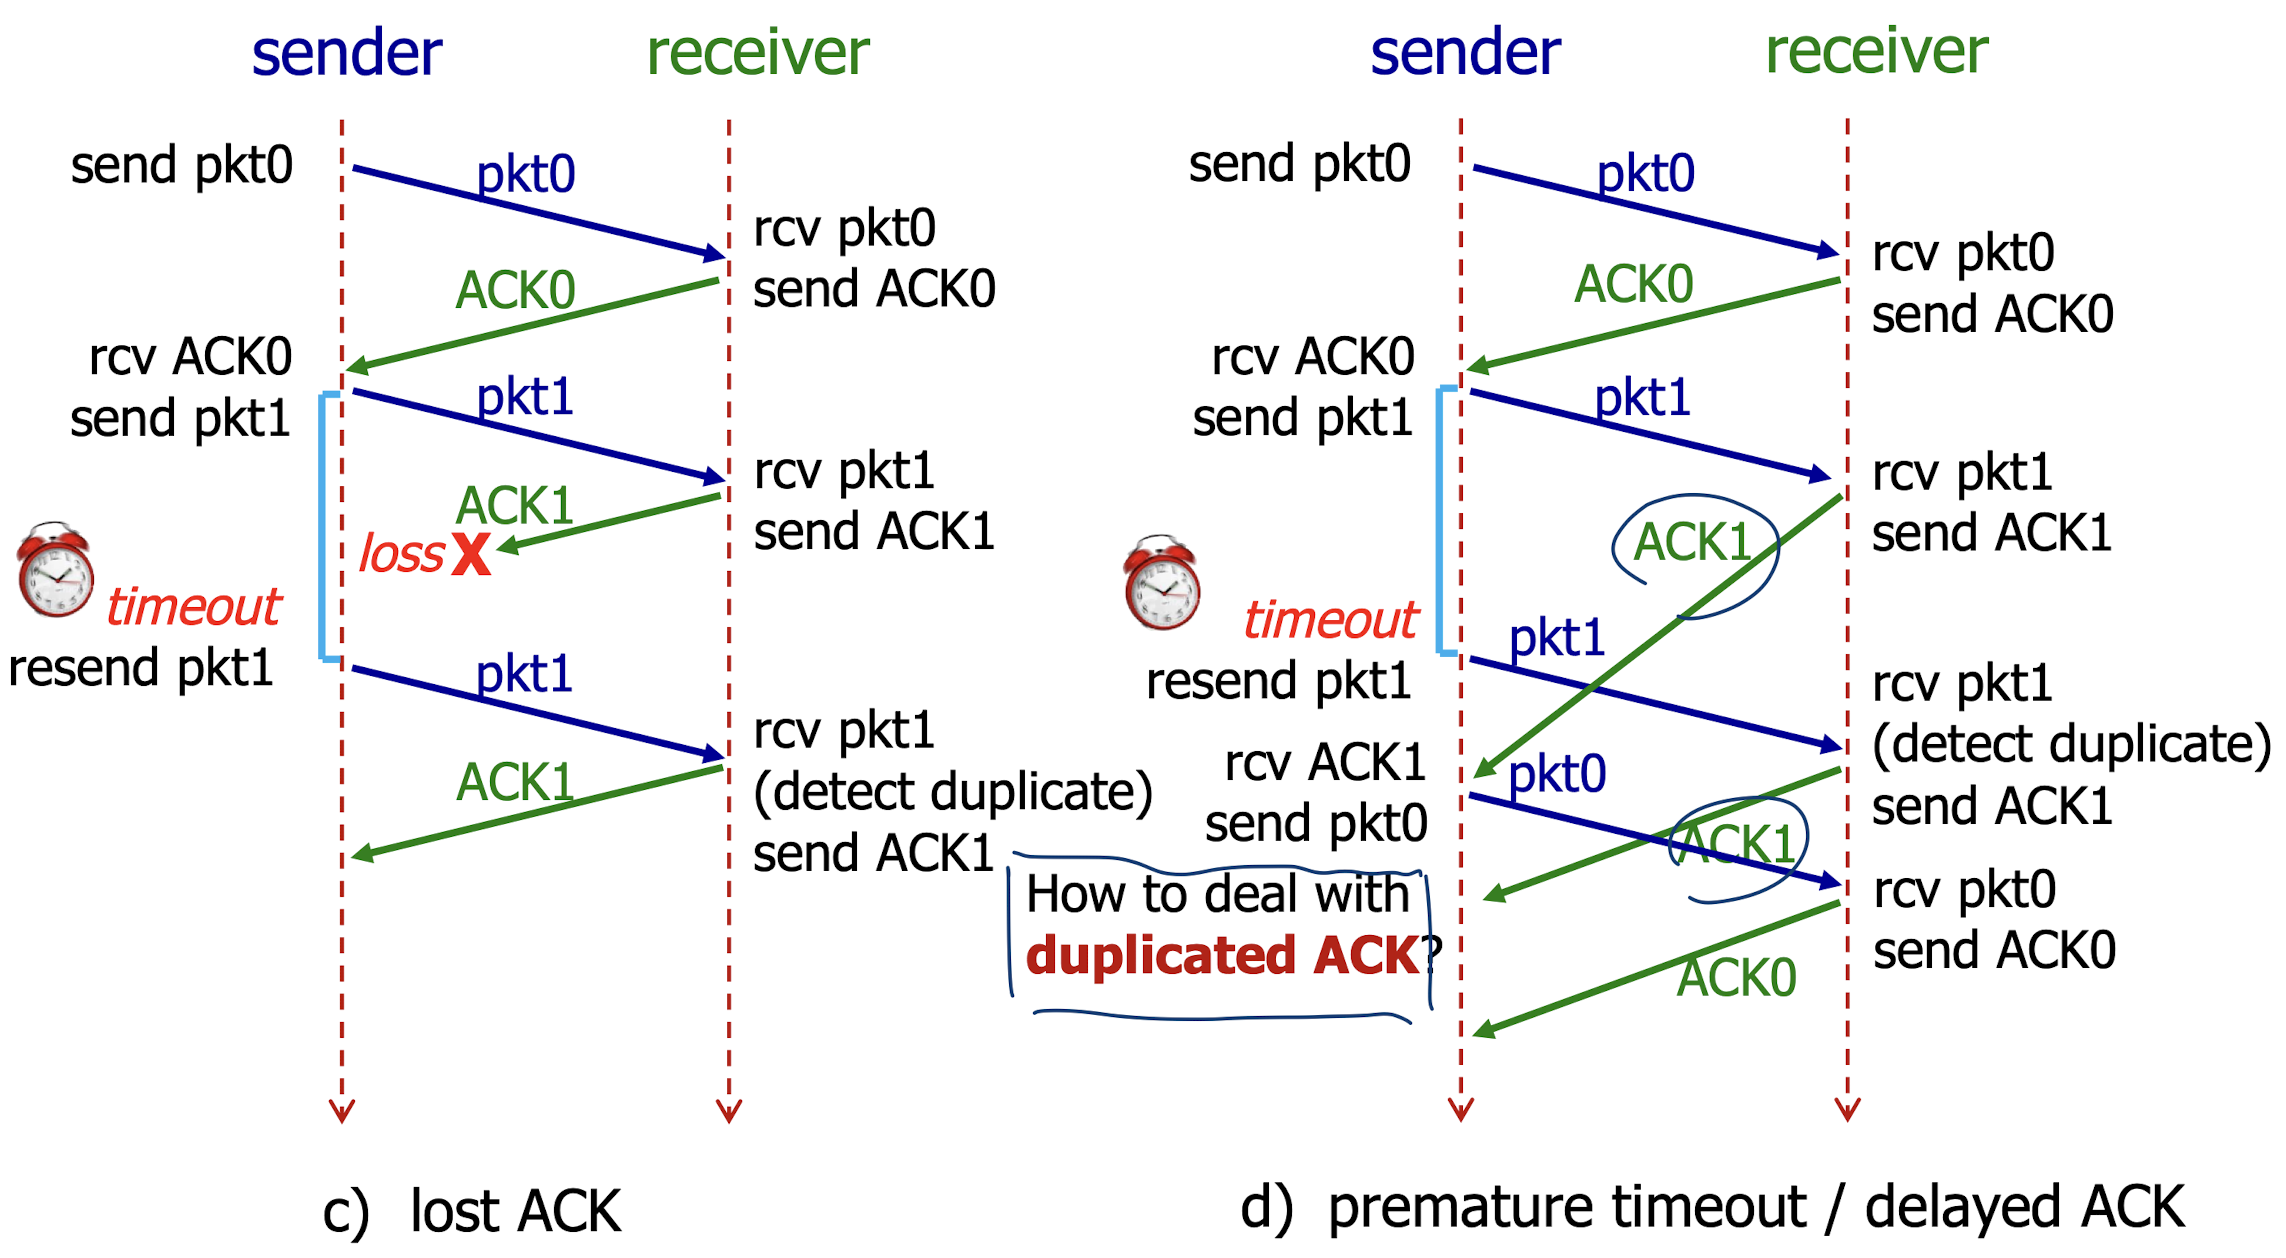
\includegraphics[scale=0.2]{rdt-3.0-1}

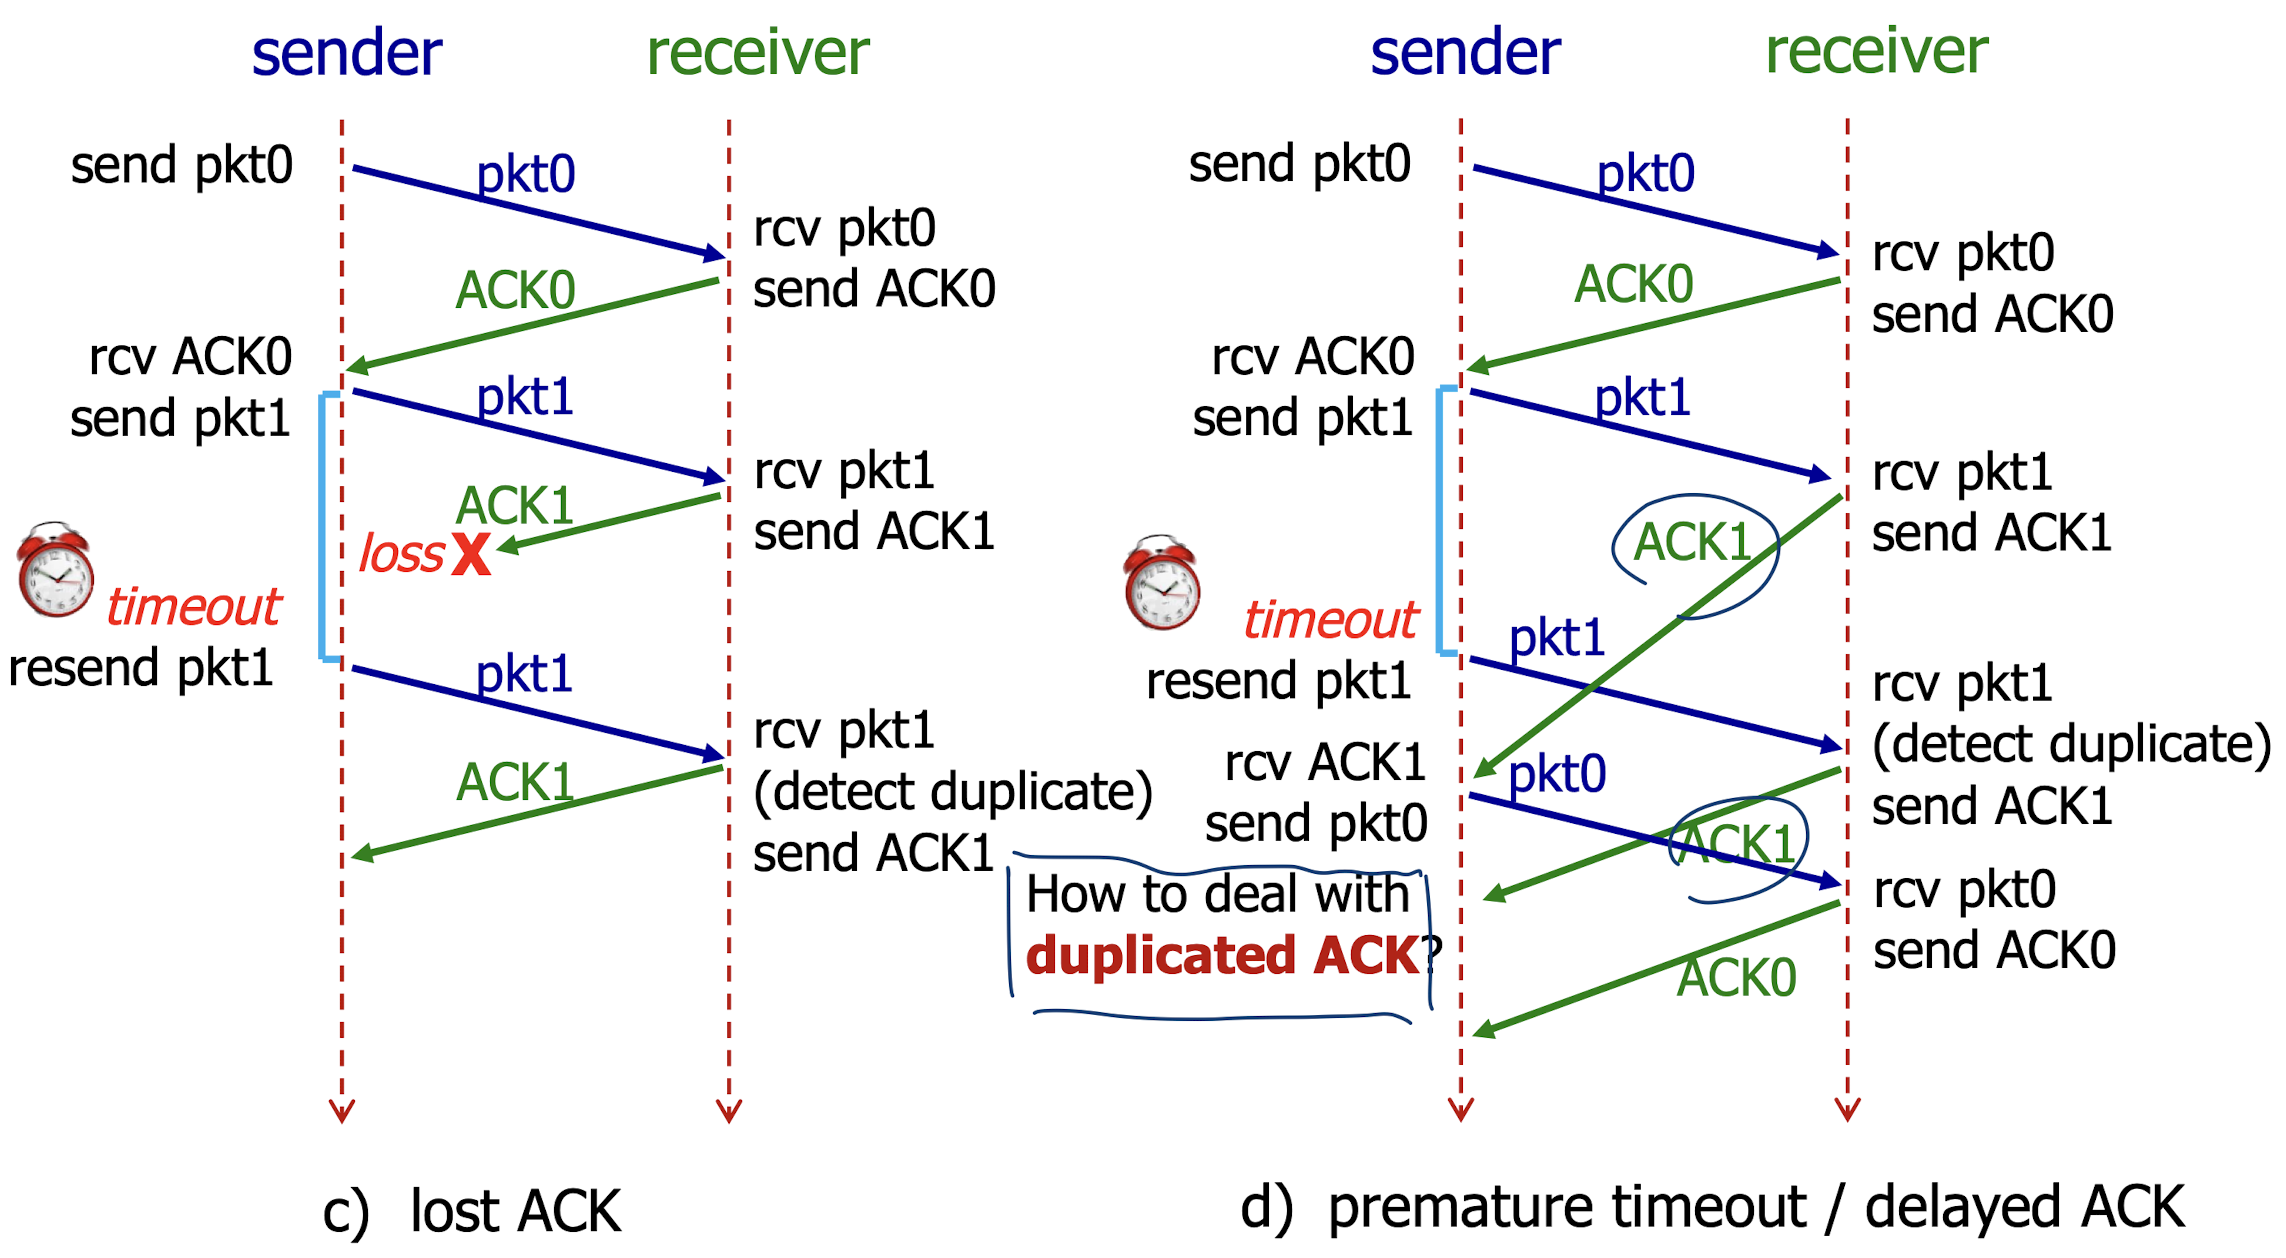
\includegraphics[scale=0.2]{rdt-3.0-2}

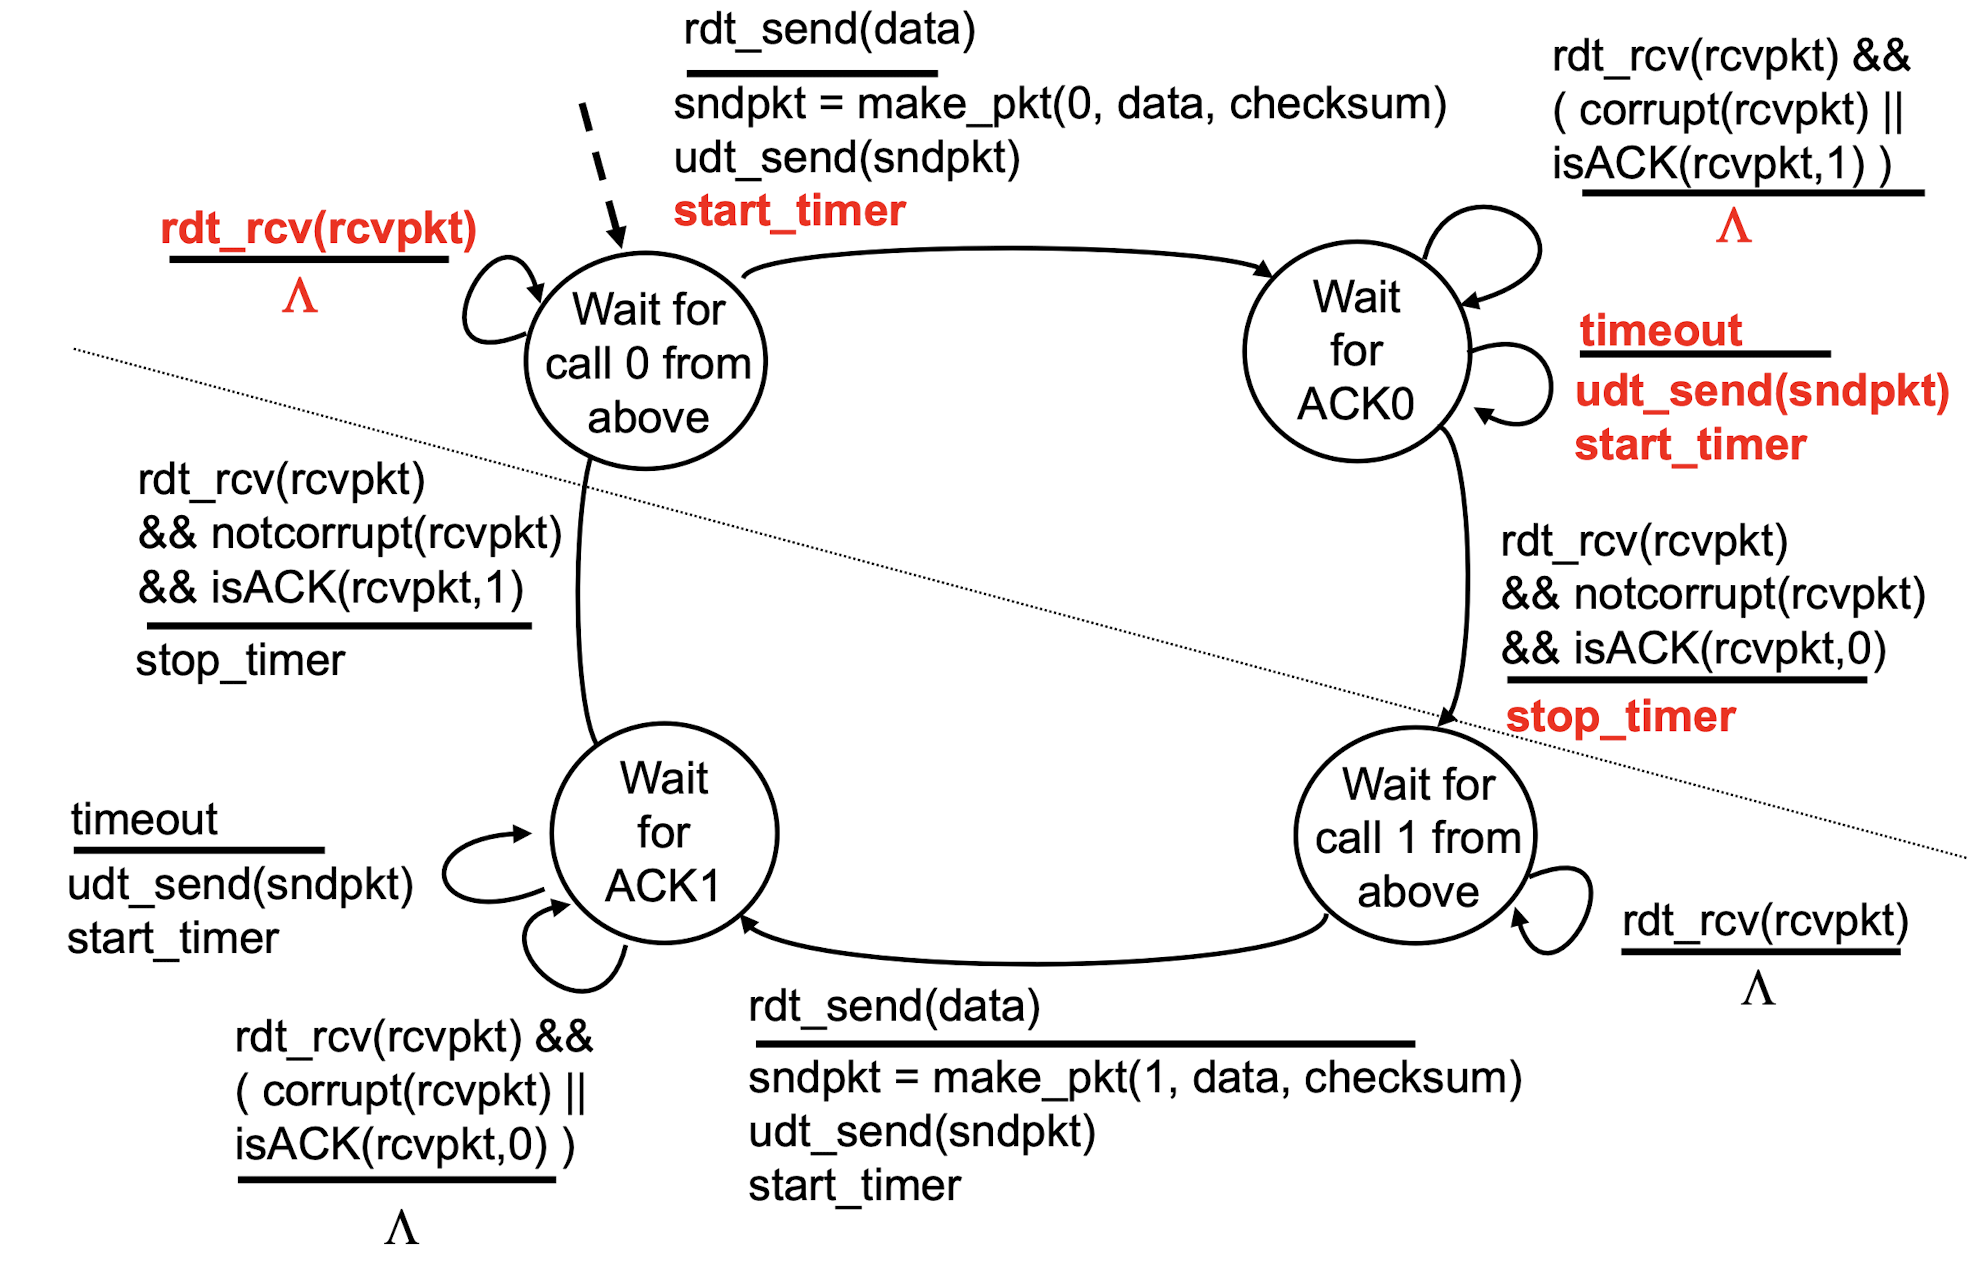
\includegraphics[scale=0.2]{rdt-3.0-fsm}

\subsubsection{Performance of rdt 3.0}

\begin{itemize}
    \item \keyword{Stop-and-wait protocol}{Sender sends 1 packet at a time, then waits for receiver response}
    \item Performance is bad. Stop-and-wait protocol limits use of resources
    \item \keyword{Utilization}{Fraction of time sender is busy sending}
    \begin{itemize}
        \item Given: 1 Gbps link, 15 ms prop. delay, 8000 bit packet
        \item $D_{trans} = \frac{L}{R} = \frac{8000 \text{ bits}}{10^9 \text{ bits/sec}} = 0.008 \text{ ms}$
        \item $U_{sender} = \frac{D_{\text{trans}}}{RTT + D_{\text{trans}}} = \frac{0.008}{30.008} = 0.027\%$
    \end{itemize}
\end{itemize}

\subsubsection{Pipelined Protocols}

\begin{itemize}
    \item \keyword{Pipelining}{Sender allows sending of multiple not-yet-ACKed packets}
    \begin{itemize}
        \item Need more sequence numbers
        \item Buffering at sender and receiver
    \end{itemize}
\end{itemize}

\subsection{Go-Back-N}

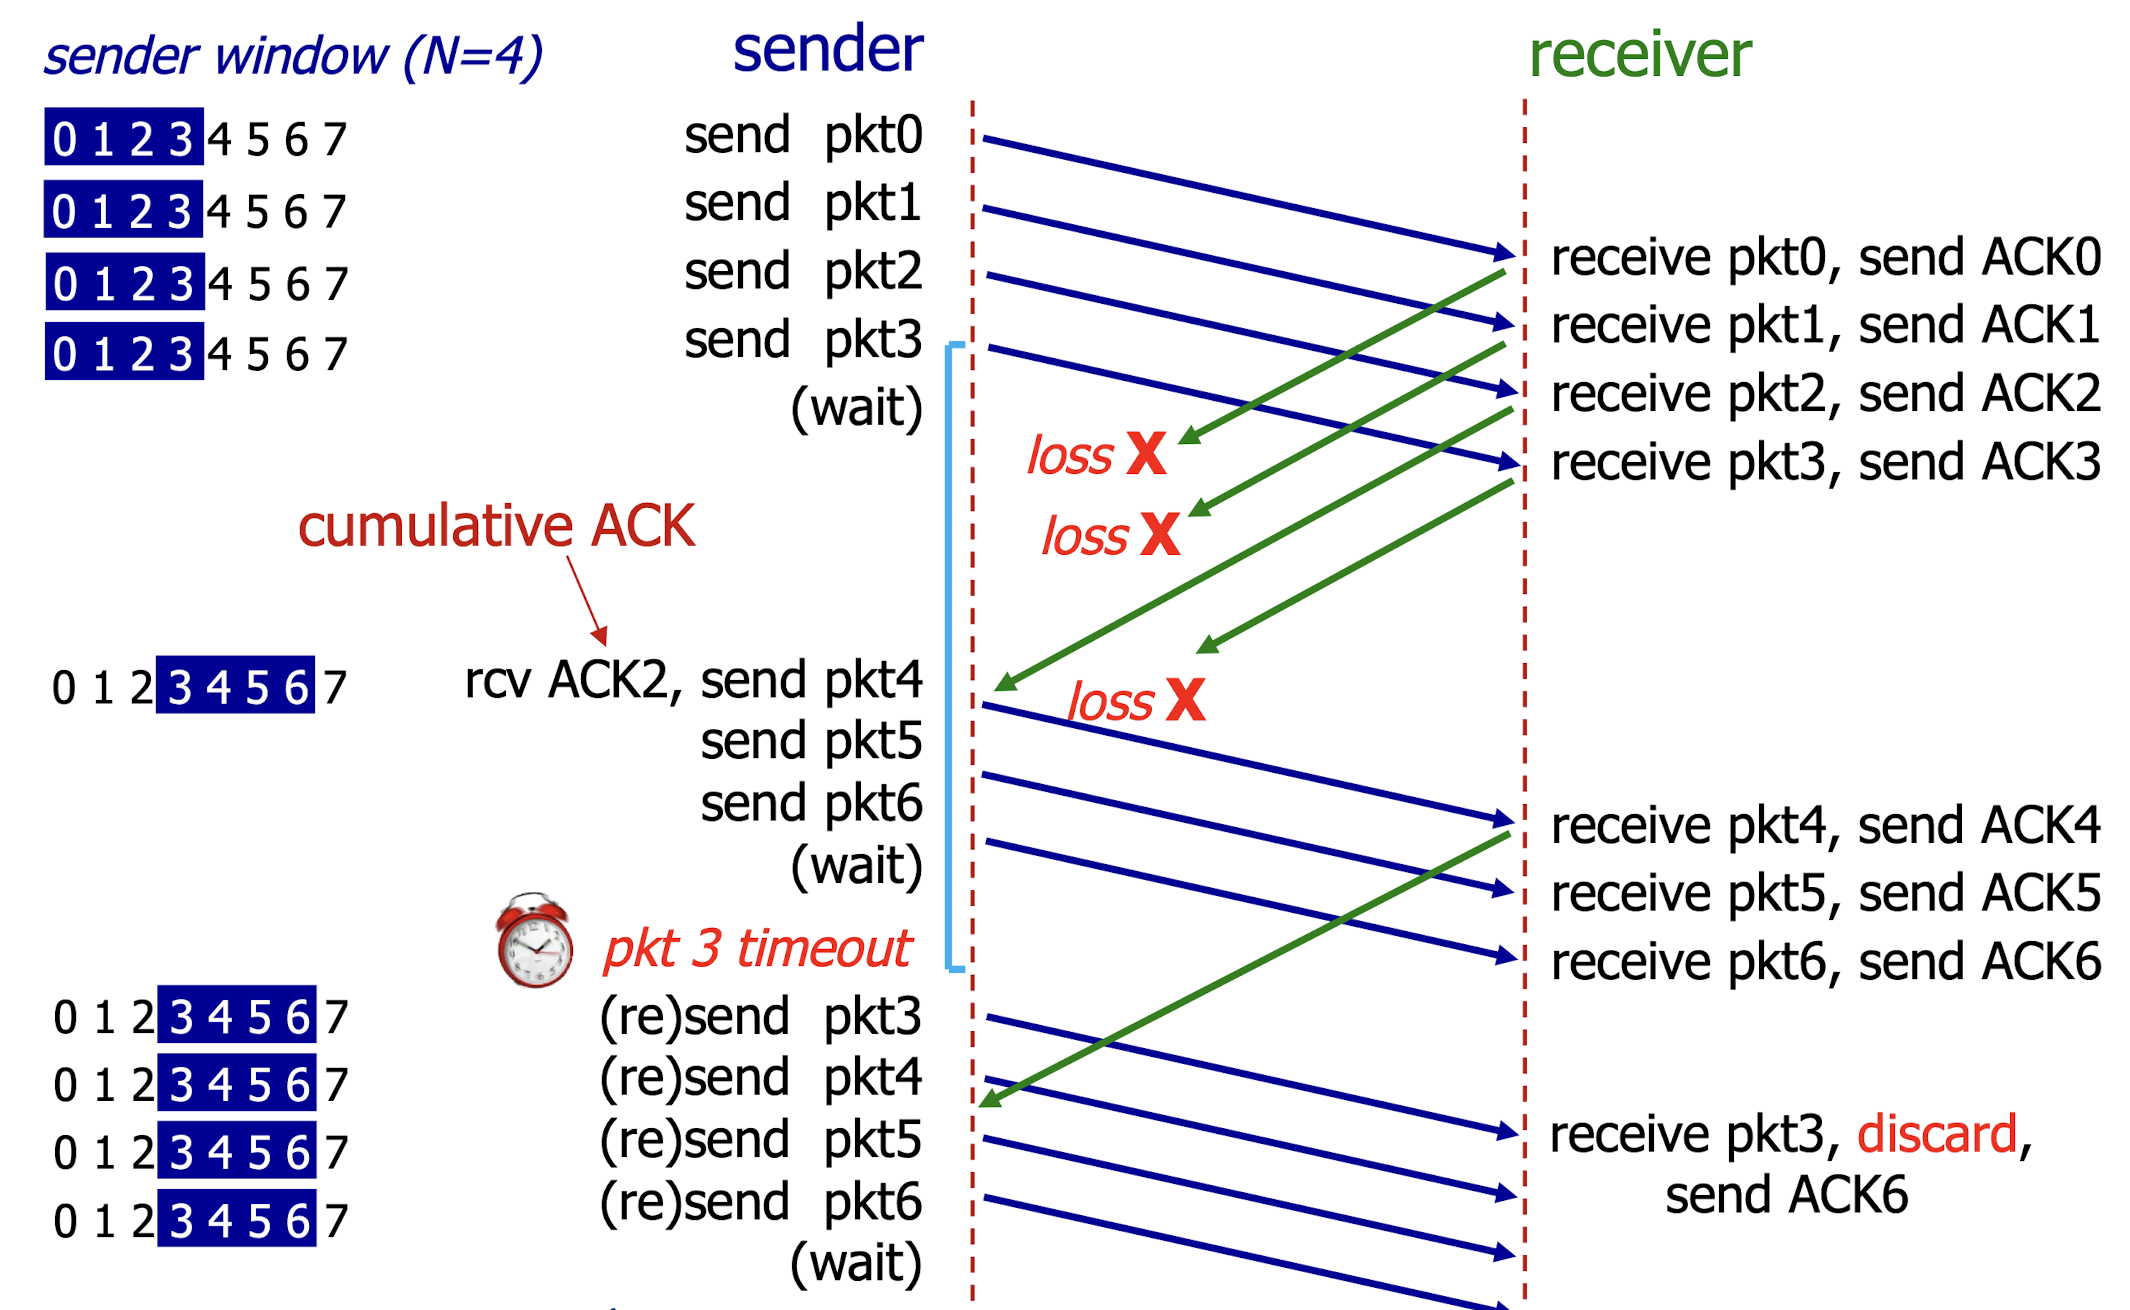
\includegraphics[scale=0.2]{go-back-n}

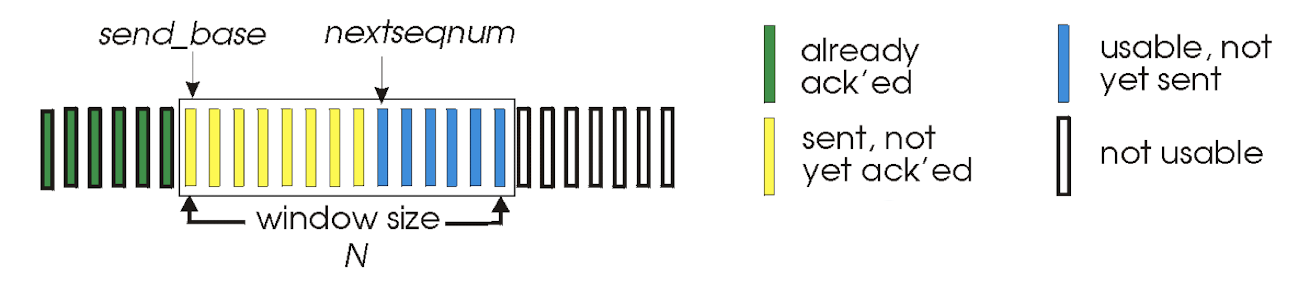
\includegraphics[scale=0.3]{go-back-n-sender}

\begin{itemize}
    \item Intuition: Sliding window
    \item Sender:
    \begin{itemize}
        \item Sends when sliding window reaches packet
        \item 1 timer to receive ACK for packet at \lstinline{send_base}
        \item If timeout($n$), retransmit packet $n$ and other pkts in window
        \item If receive ACK $n$, check if can shift sliding window. Previous un-ACKed packets guaranteed to be received.
        \item If duplicate ACK, ignore like in rdt 3.0. Retransmit only on timeout.
    \end{itemize}
    \item Receiver:
    \begin{itemize}
        \item \keyword{Cumulative ACK}{ACK for correct pkt with highest in-order sequence}
        \item Discard out-of-order packets
    \end{itemize}
    \item Not efficient, since future packets discarded if pkt lost and out-of-order
\end{itemize}

\subsection{Selective Repeat}

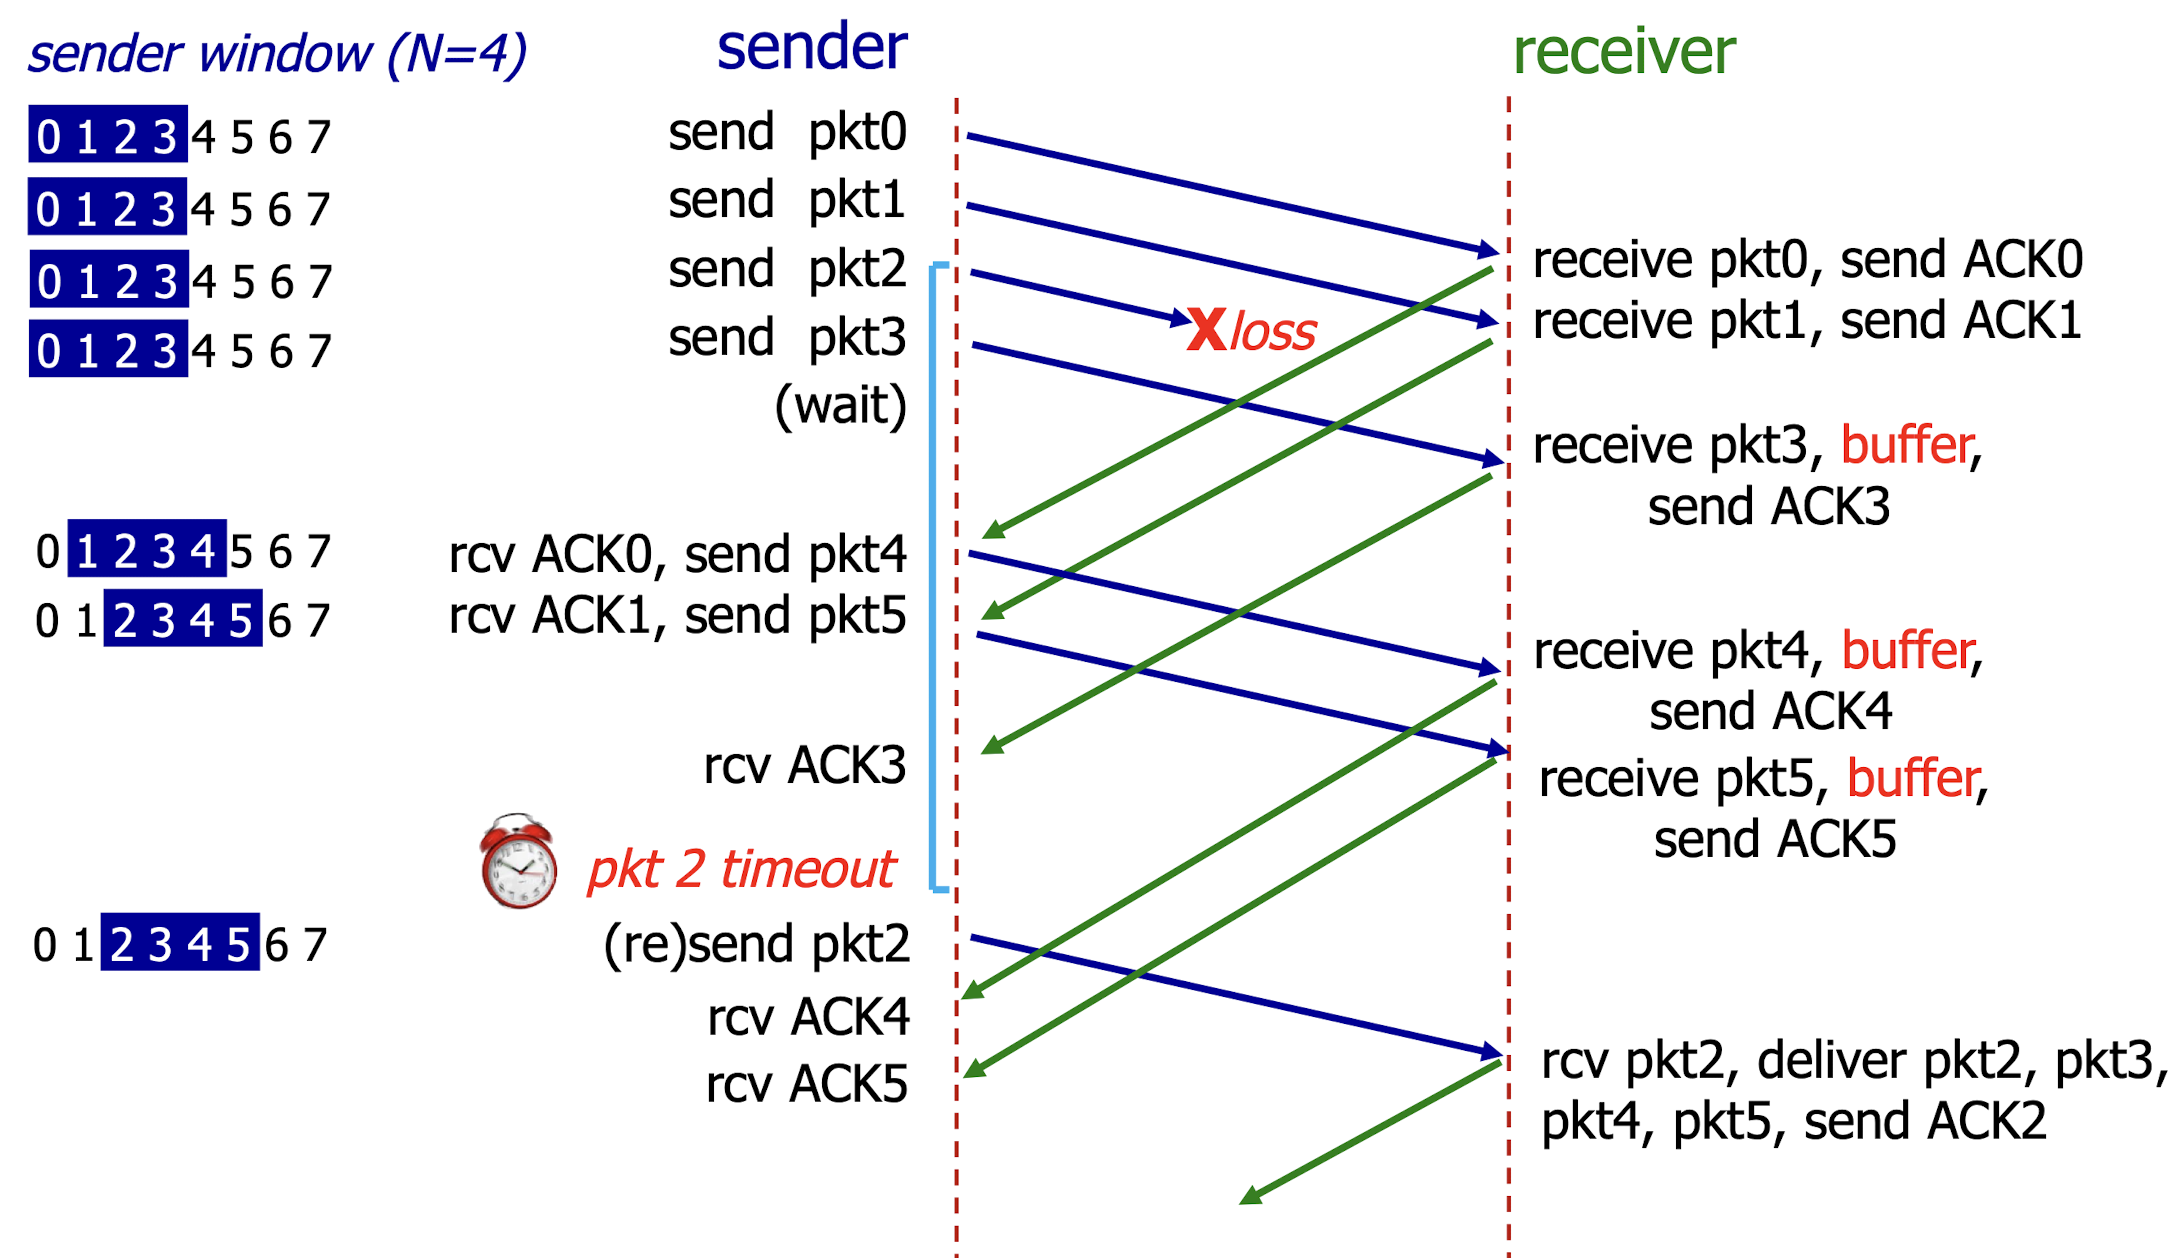
\includegraphics[scale=0.2]{selective-repeat}

\begin{itemize}
    \item Receiver individually ACKs correct pkts (Not accumulative) and sender maintains timer for each unACKed pkt
    \item Sender:
    \begin{itemize}
        \item If timeout($n$), retransmit packet $n$ only
        \item If ACK($n$) and $n$ is smallest unACKed pkt, slide window
    \end{itemize}
    \item Receiver:
    \begin{itemize}
        \item Once receive pkt $n$ in window, send ACK($n$). If out-of-order, buffer. If in-order, deliver and slide window
        \item Once receive pkt $n$ outside of window, still send ACK($n$)
    \end{itemize}
\end{itemize}

\subsection{Summary}

\begin{tabular}{ |p{15pt}|p{105pt}|p{105pt}| }
    \hline
    \textbf{rdt} & \textbf{New problems} & \textbf{New features} \\
    \hline
    \textbf{1.0} & n/a & n/a \\
    \hline
    \textbf{2.0} & Bit error in data & Sender: Checksum, Receiver: ACK/NAK \\
    \hline
    \textbf{2.1} & Bit error in feedback, Duplicate packets & Receiver: Checksum, Sender: Sequence number \\
    \hline
    \textbf{2.2} & Remove NAK & Receiver: Sequence number \\
    \hline
    \textbf{3.0} & Packet loss in data and feedback & Timeout, Re-transmission \\
    \hline
\end{tabular}

\section{05. TCP}

\begin{itemize}
    \item Point-to-point: 1 sender and 1 receiver
    \item Connection-oriented
    \item Full duplex data: Data and feedback can be sent together both ways
    \begin{itemize}
        \item Before in UDP: Data only goes 1 way
    \end{itemize}
    \item Reliable, in-order \textbf{byte stream} (segment)
    \begin{itemize}
        \item Before in UDP: Send packet by packet
    \end{itemize}
    \item Pipelined: \textbf{Dynamic window size} set by flow control
\end{itemize}

\subsection{Buffers and Segments}

\begin{itemize}
    \item Sender and receiver both have 2 buffers to send and receive data
    \item \keyword{Maximum Segment Size}{(MSS) Usually 1460 bytes. Limited by max. transmission unit (MTU)}
\end{itemize}

\subsection{Segment Structure}

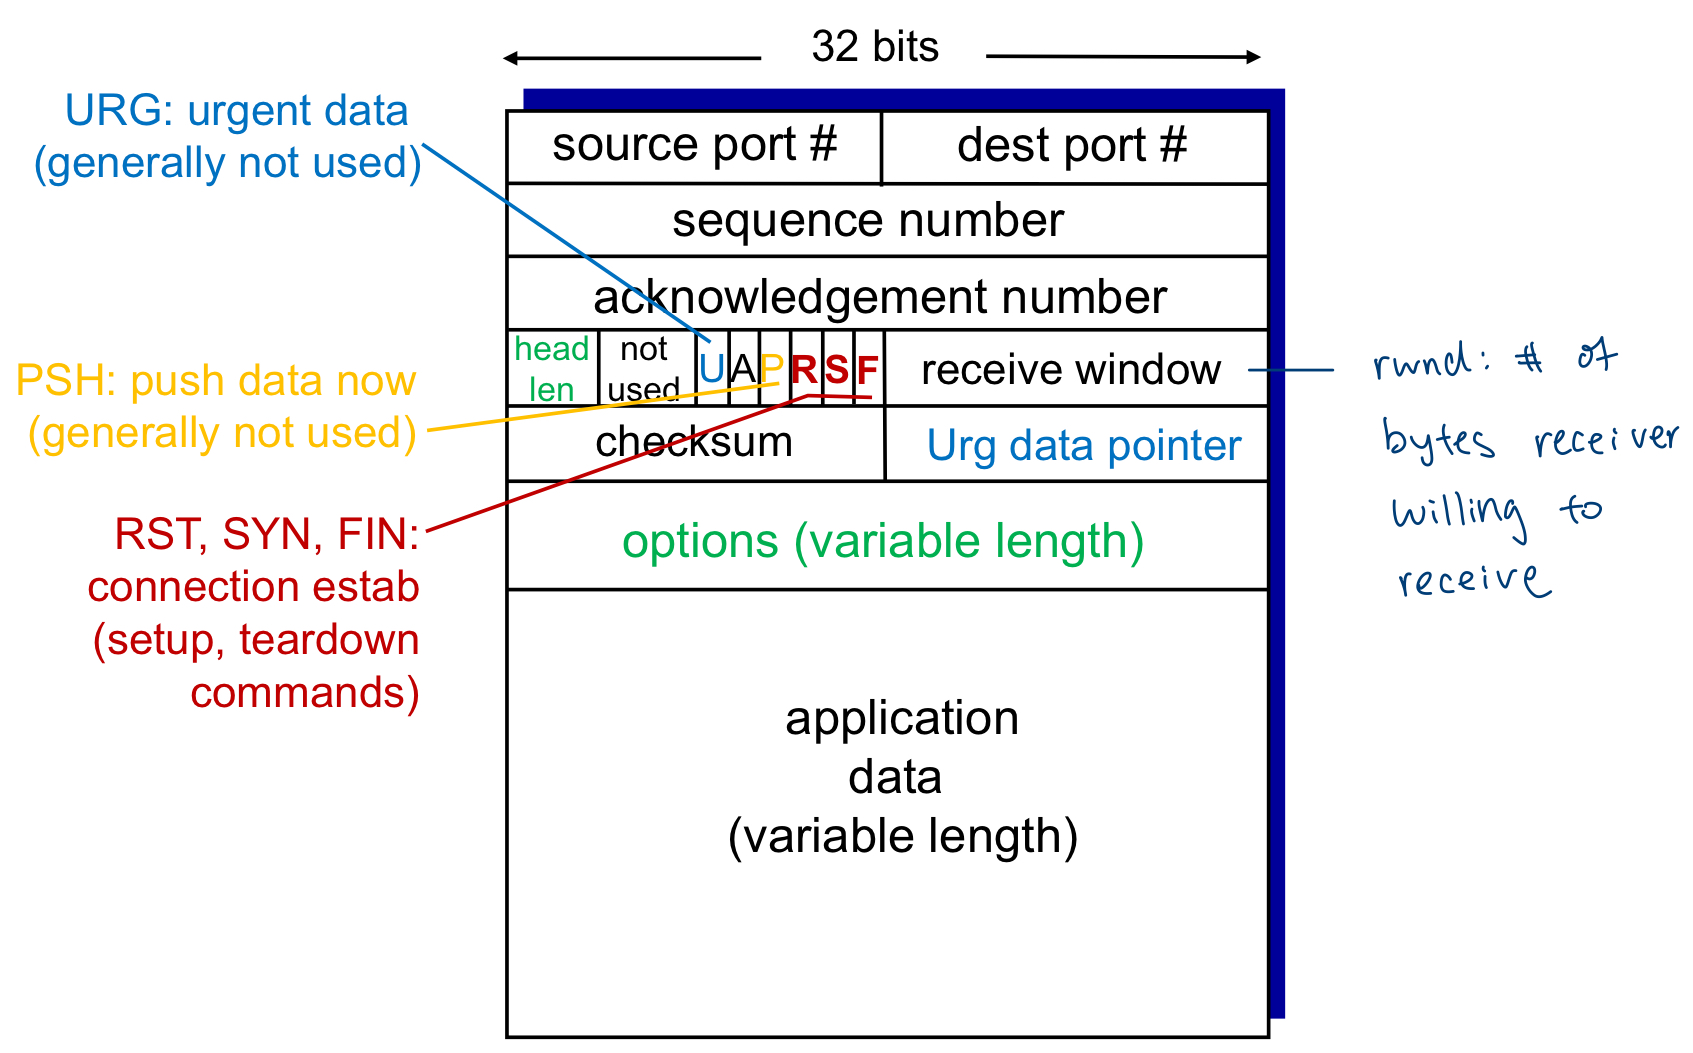
\includegraphics[scale=0.1]{tcp-segment-structure}

\begin{itemize}
    \item Source/Dest. Port Number: Same as UDP, except ports can be demultiplexed to different sockets
    \item \keyword{Sequence Number}{Byte number of first byte of data in segment}
    \item \keyword{Acknowledgement Number}{Sequence number of \textbf{next byte expected} from other side (Diff. from UDP)}
\end{itemize}

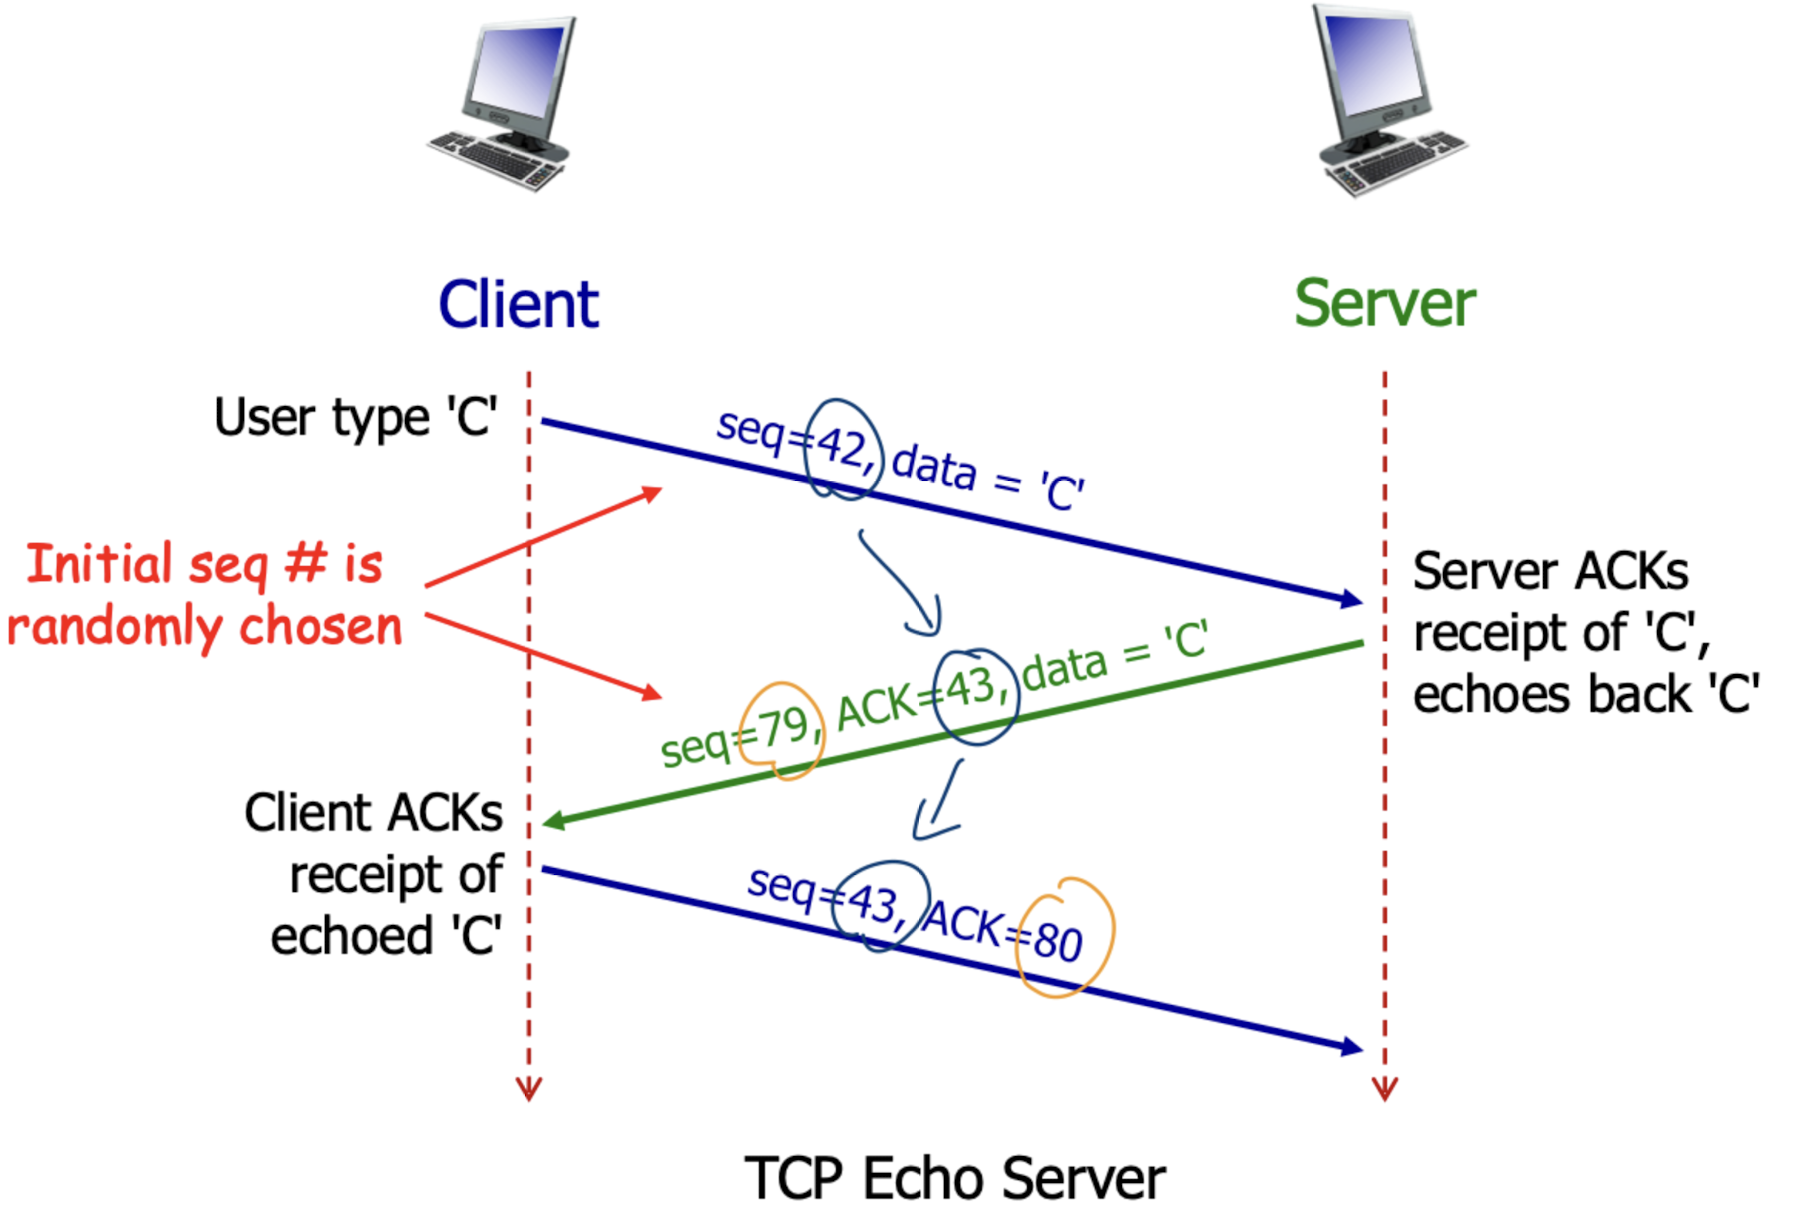
\includegraphics[scale=0.2]{tcp-sequence-and-ack-num}

\begin{itemize}
    \item \keyword{Receive Window}{For flow control. Receiver controls sender, so sender won't overflow receiver's buffer. Constrains sliding window.}
\end{itemize}

\subsection{Connection Management}

\subsubsection{3 Way Handshake}

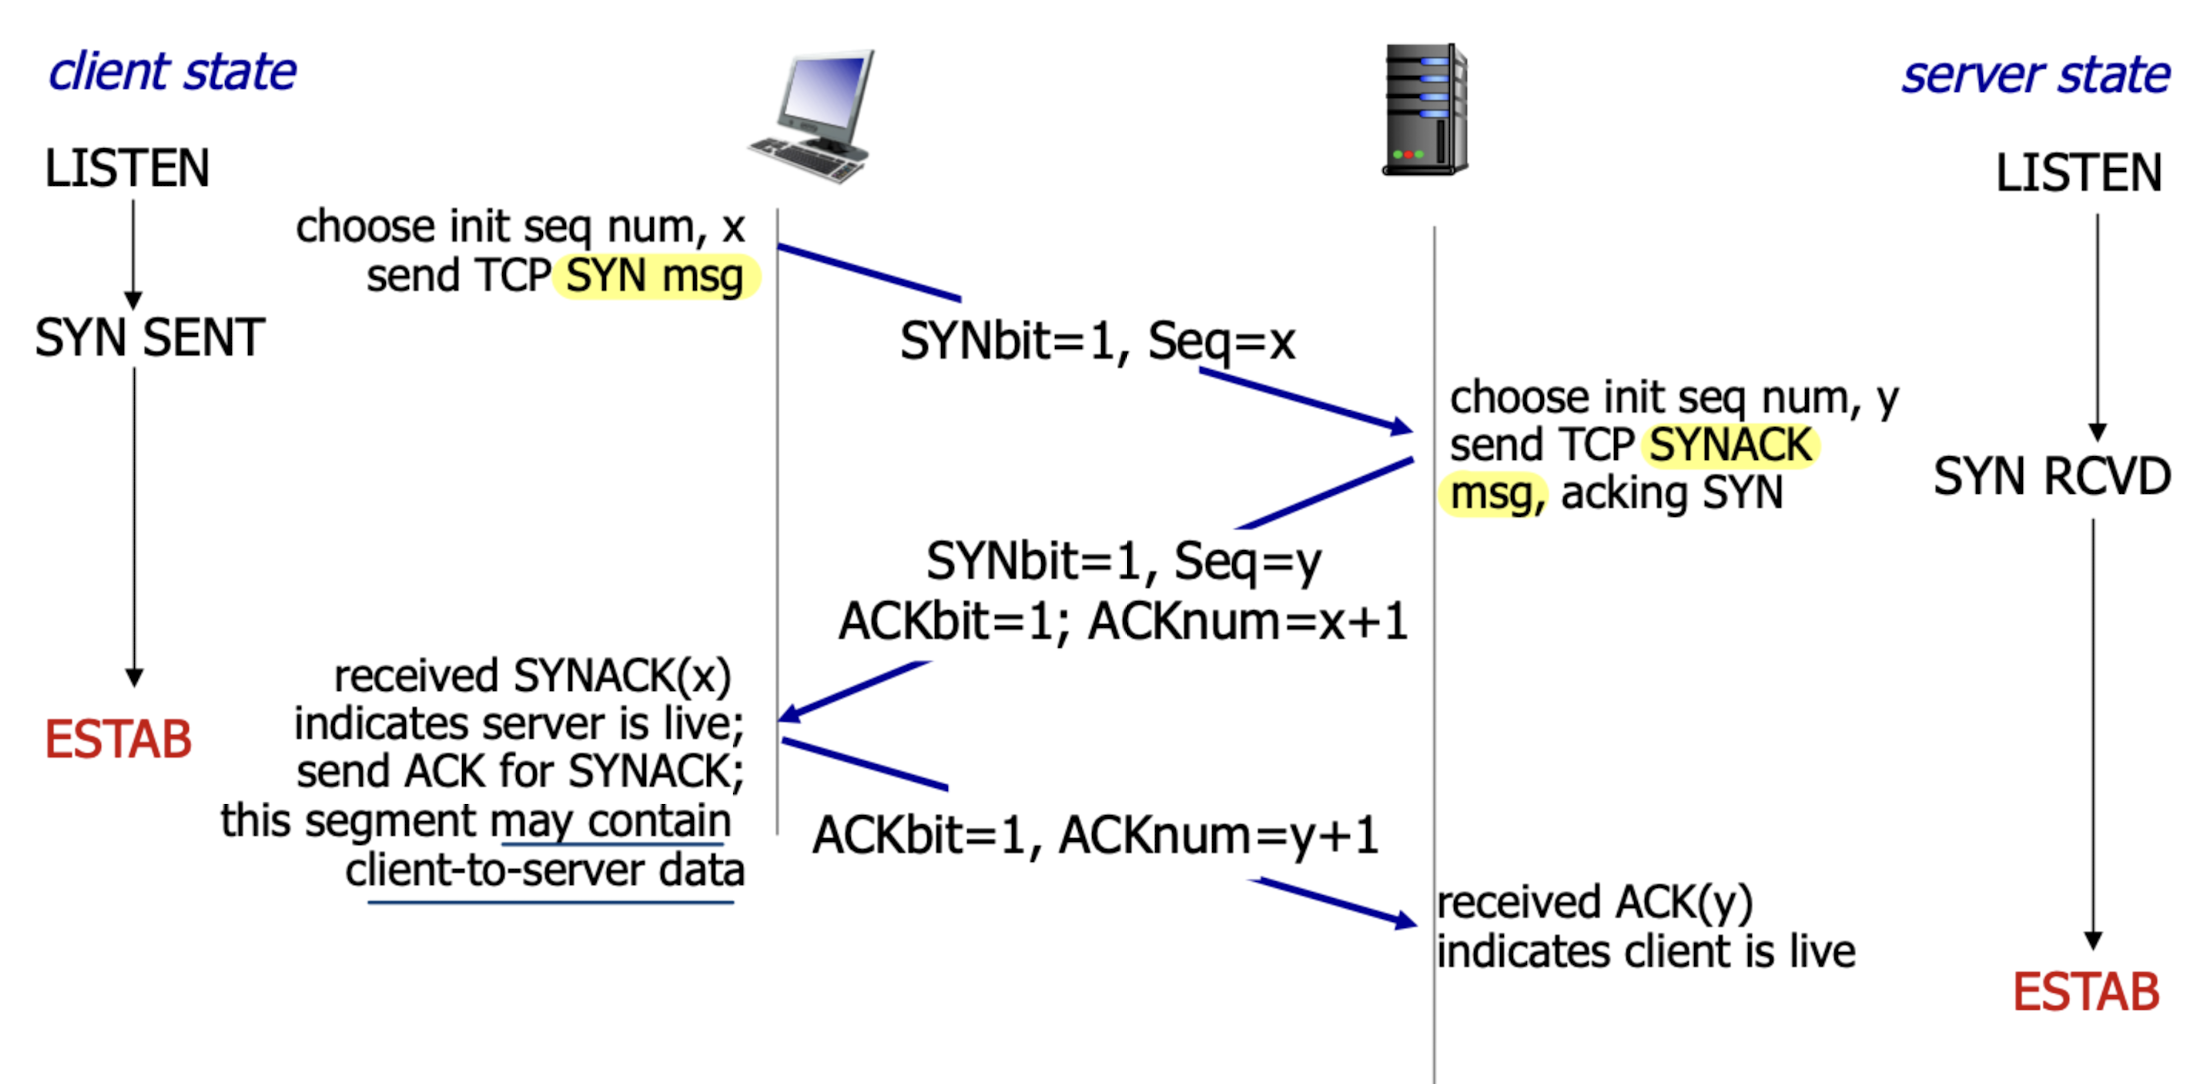
\includegraphics[scale=0.2]{tcp-3-way-handshake}

\subsubsection{Closing a Connection}

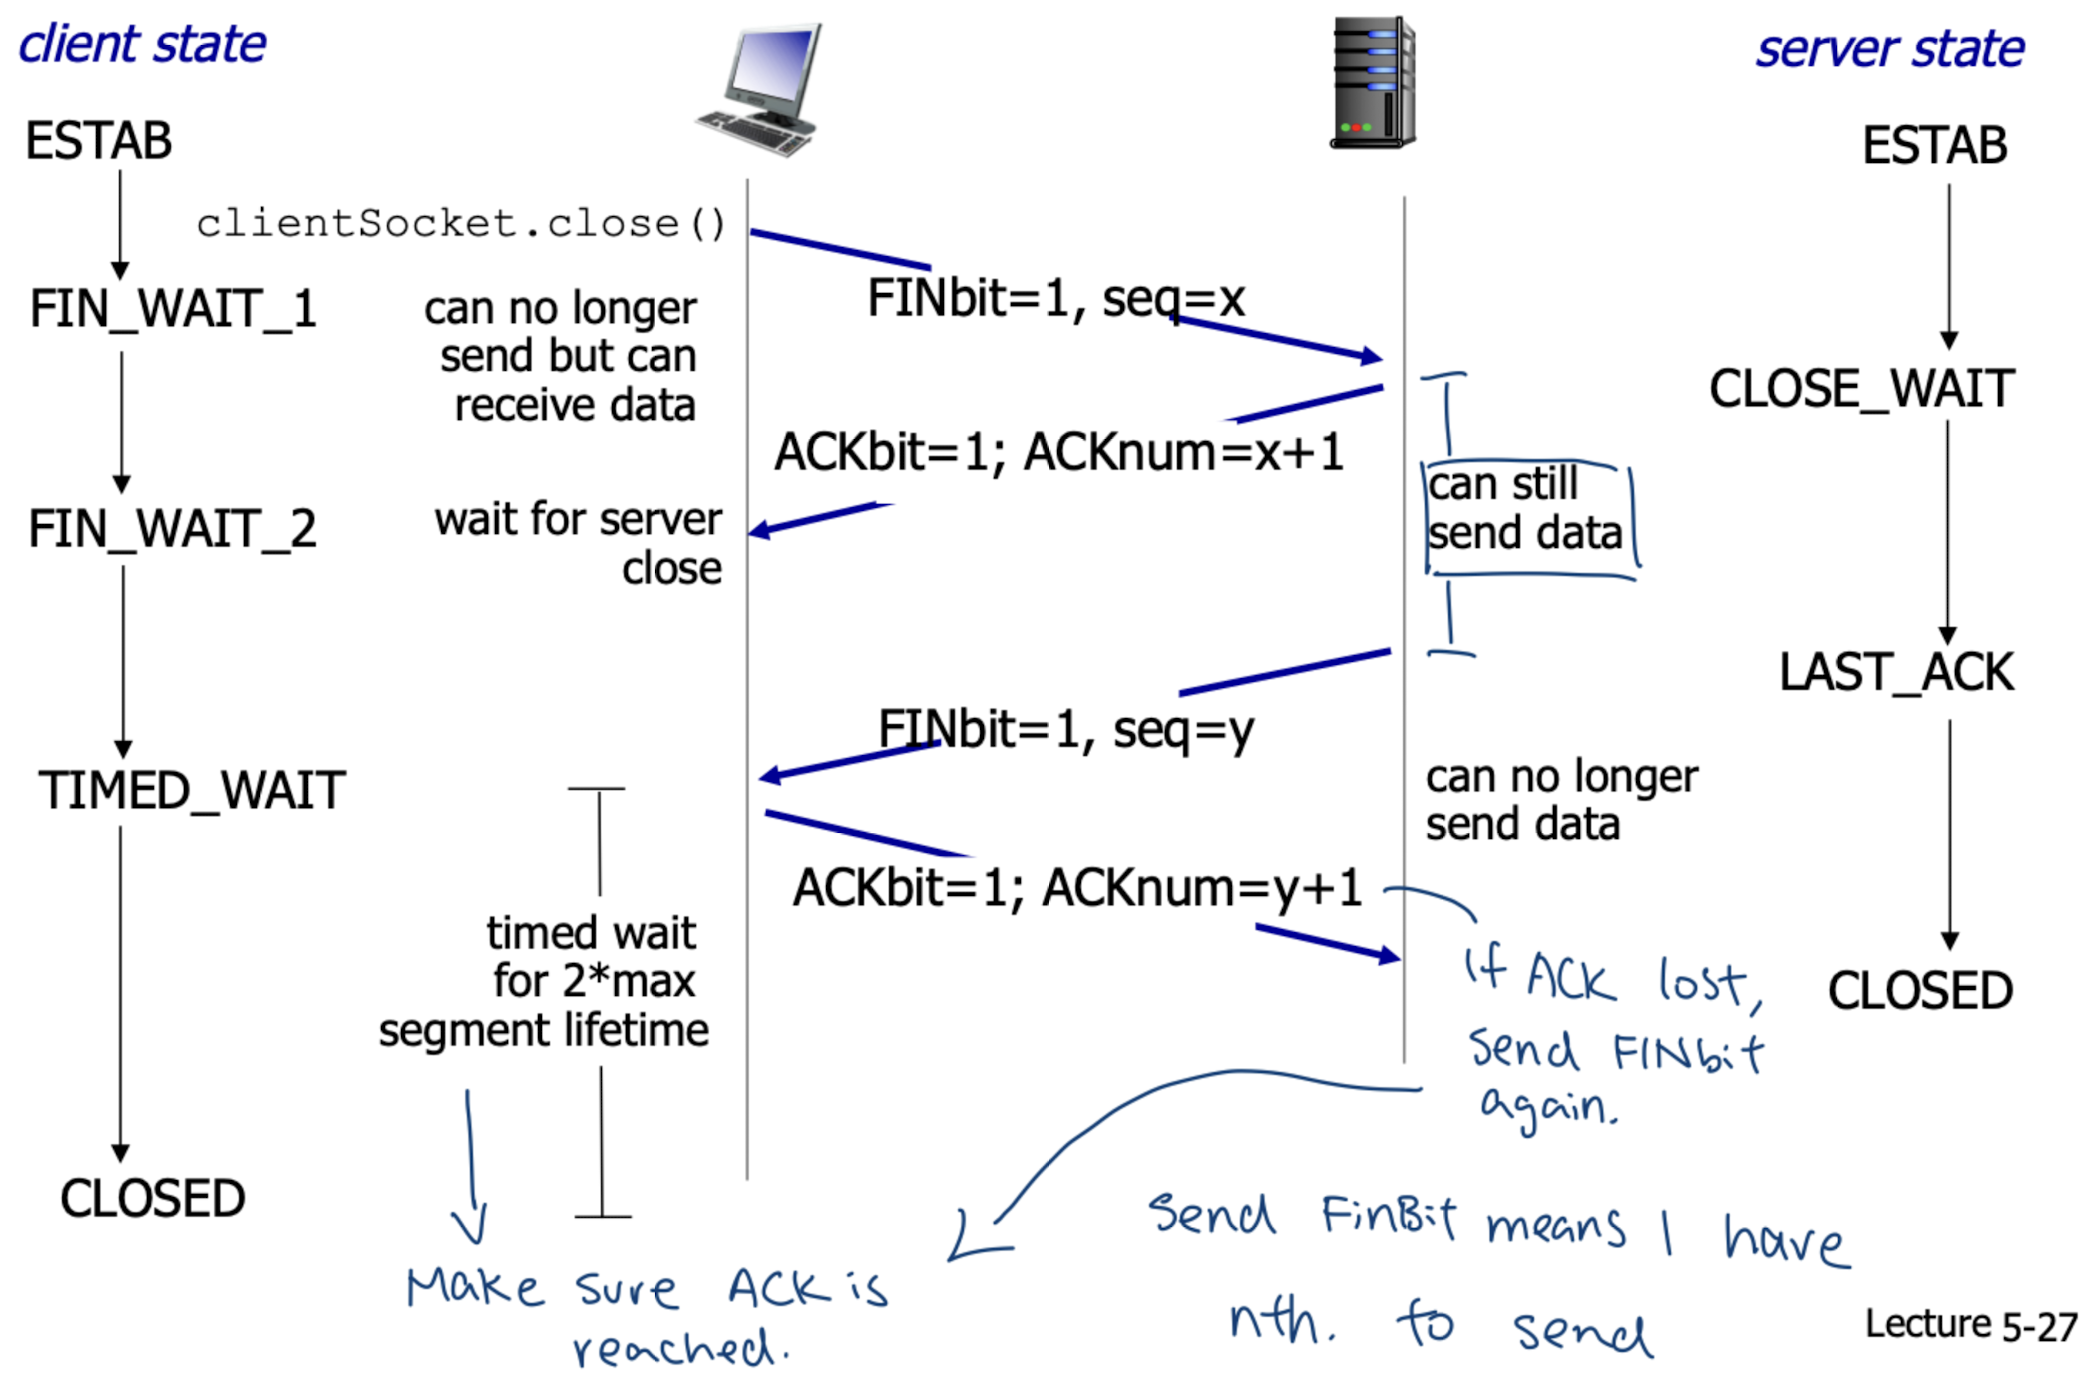
\includegraphics[scale=0.2]{tcp-close-connection}

\subsection{Reliable Data Transfer}

\begin{itemize}
    \item On top of UDT service, TCP adds:
    \begin{itemize}
        \item Pipelined segments
        \item Cumulative ACKs
        \item Single retransmission timer
    \end{itemize}
    \item Out-of-order packets not specified in TCP. Up to implementer.
    \item Retransmits on timeout or 4 duplicate ACKs
\end{itemize}

\subsubsection{Sender Events}

\begin{itemize}
    \item If data received from application:
    \begin{itemize}
        \item Create segment with sequence number
        \item Start timer for \textbf{oldest un-ACKed segment}
    \end{itemize}
    \item If timeout:
    \begin{itemize}
        \item Retransmit segment causing timeout (Similar to selective repeat)
        \item Restart timer
    \end{itemize}
    \item If ACK received:
    \begin{itemize}
        \item If ACK acknowledges previously un-ACKed segments, update window and start timer. 
    \end{itemize}
\end{itemize}

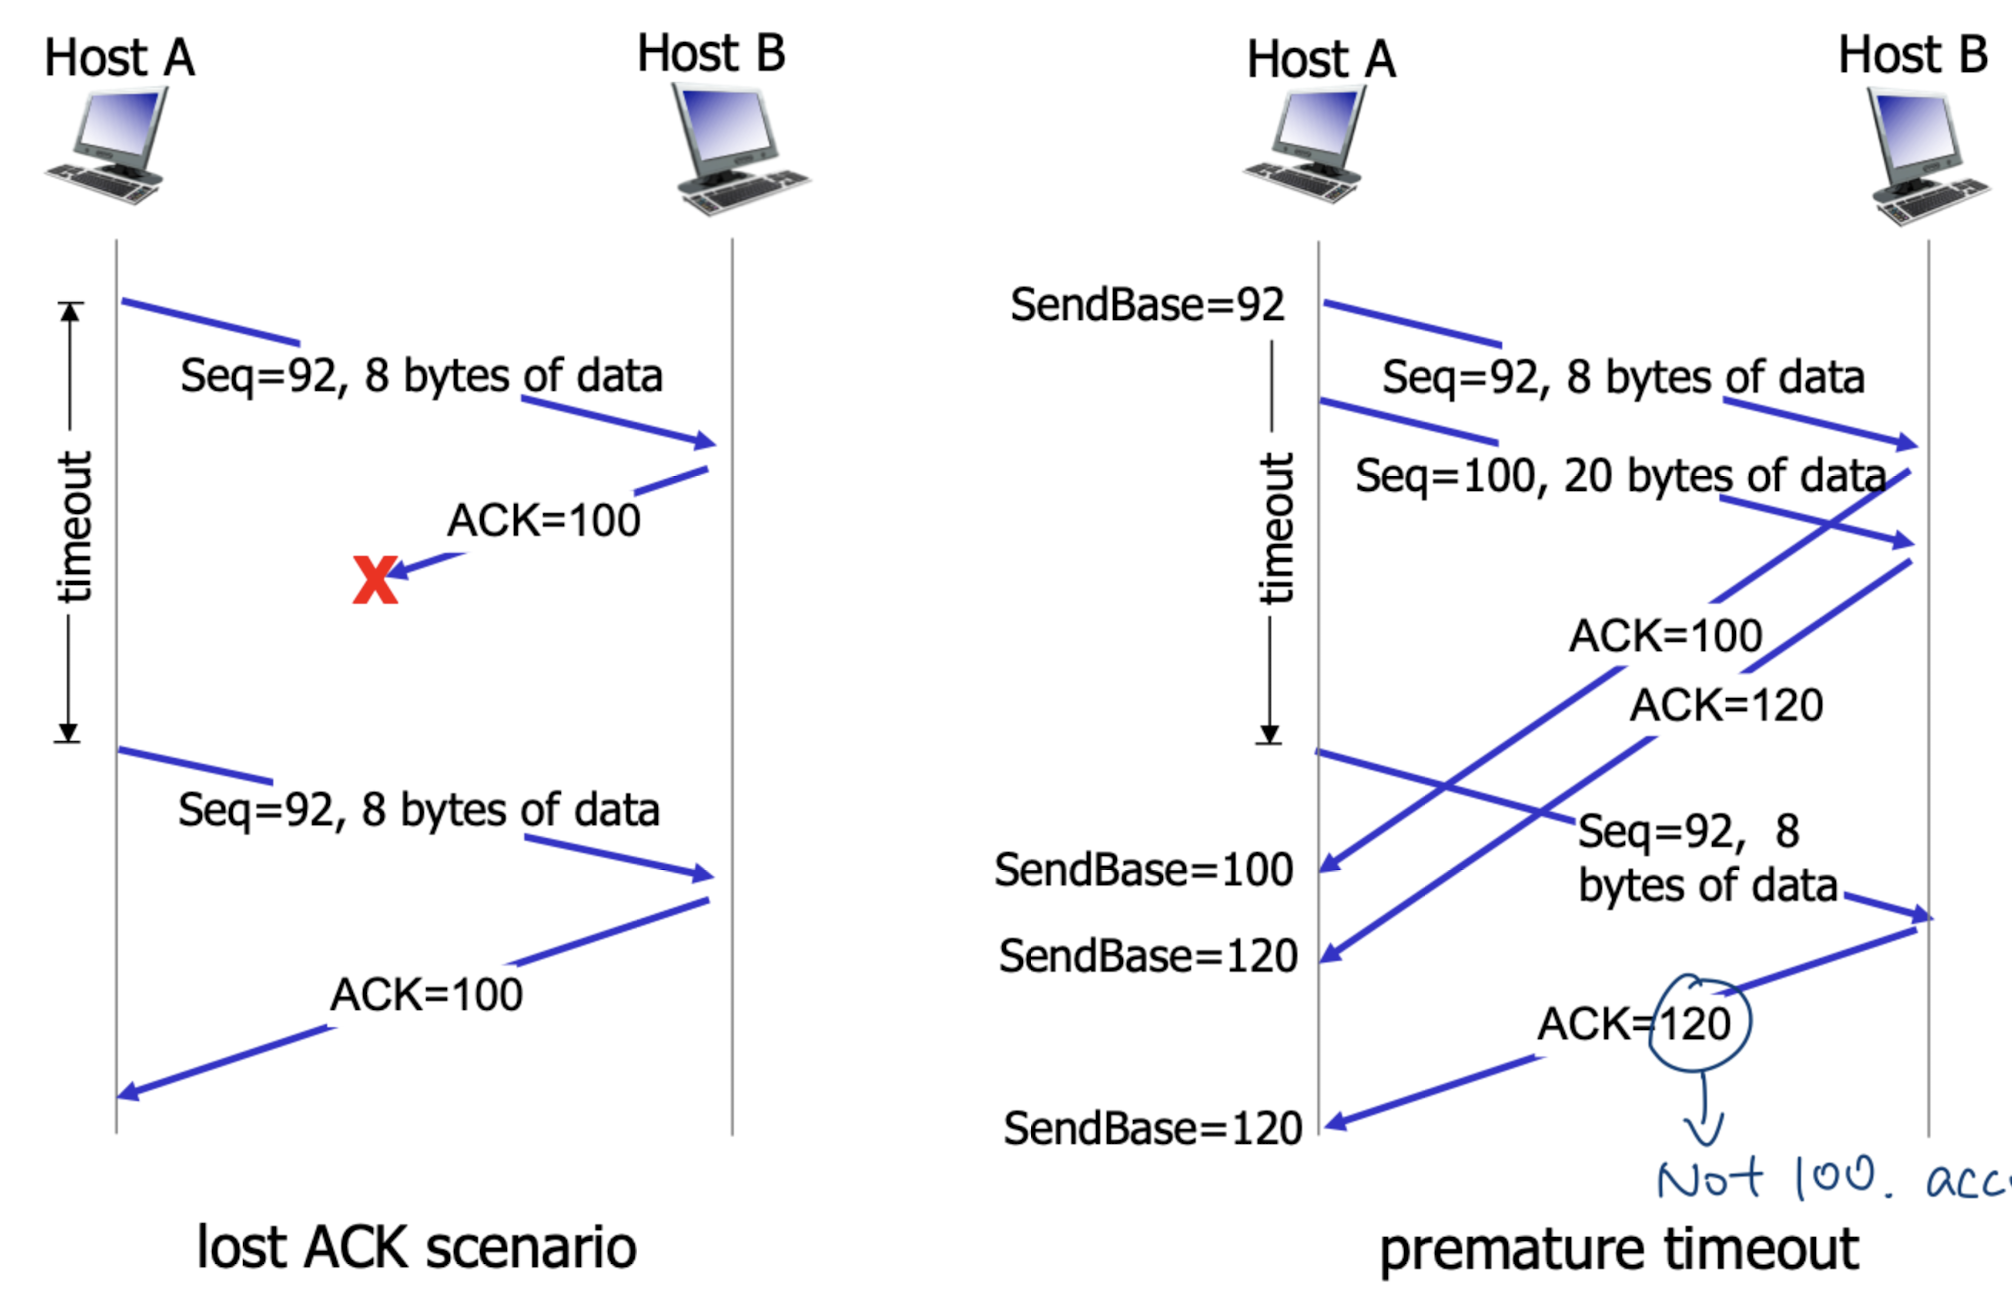
\includegraphics[scale=0.2]{tcp-retransmission-1}

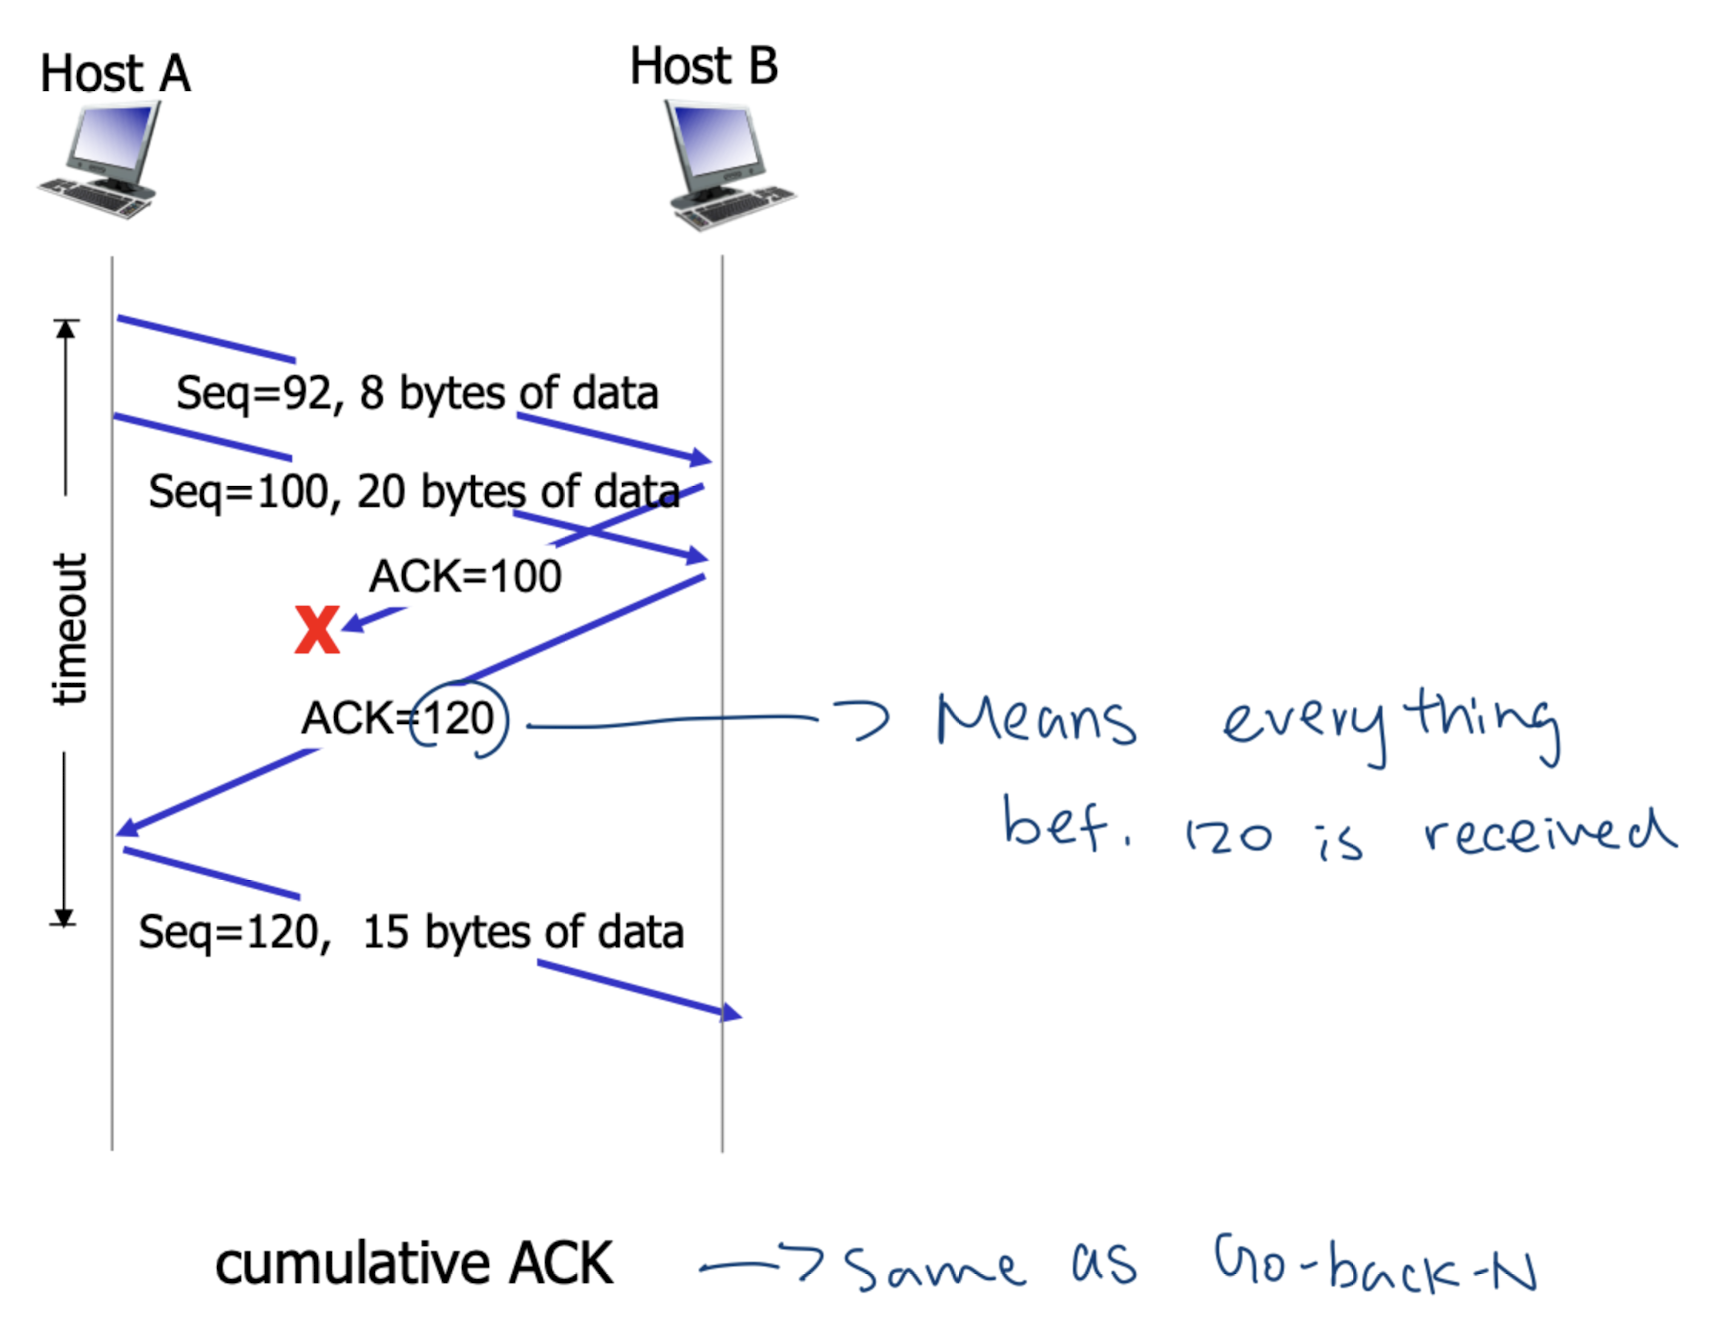
\includegraphics[scale=0.2]{tcp-retransmission-2}

\subsubsection{Receiver Events}

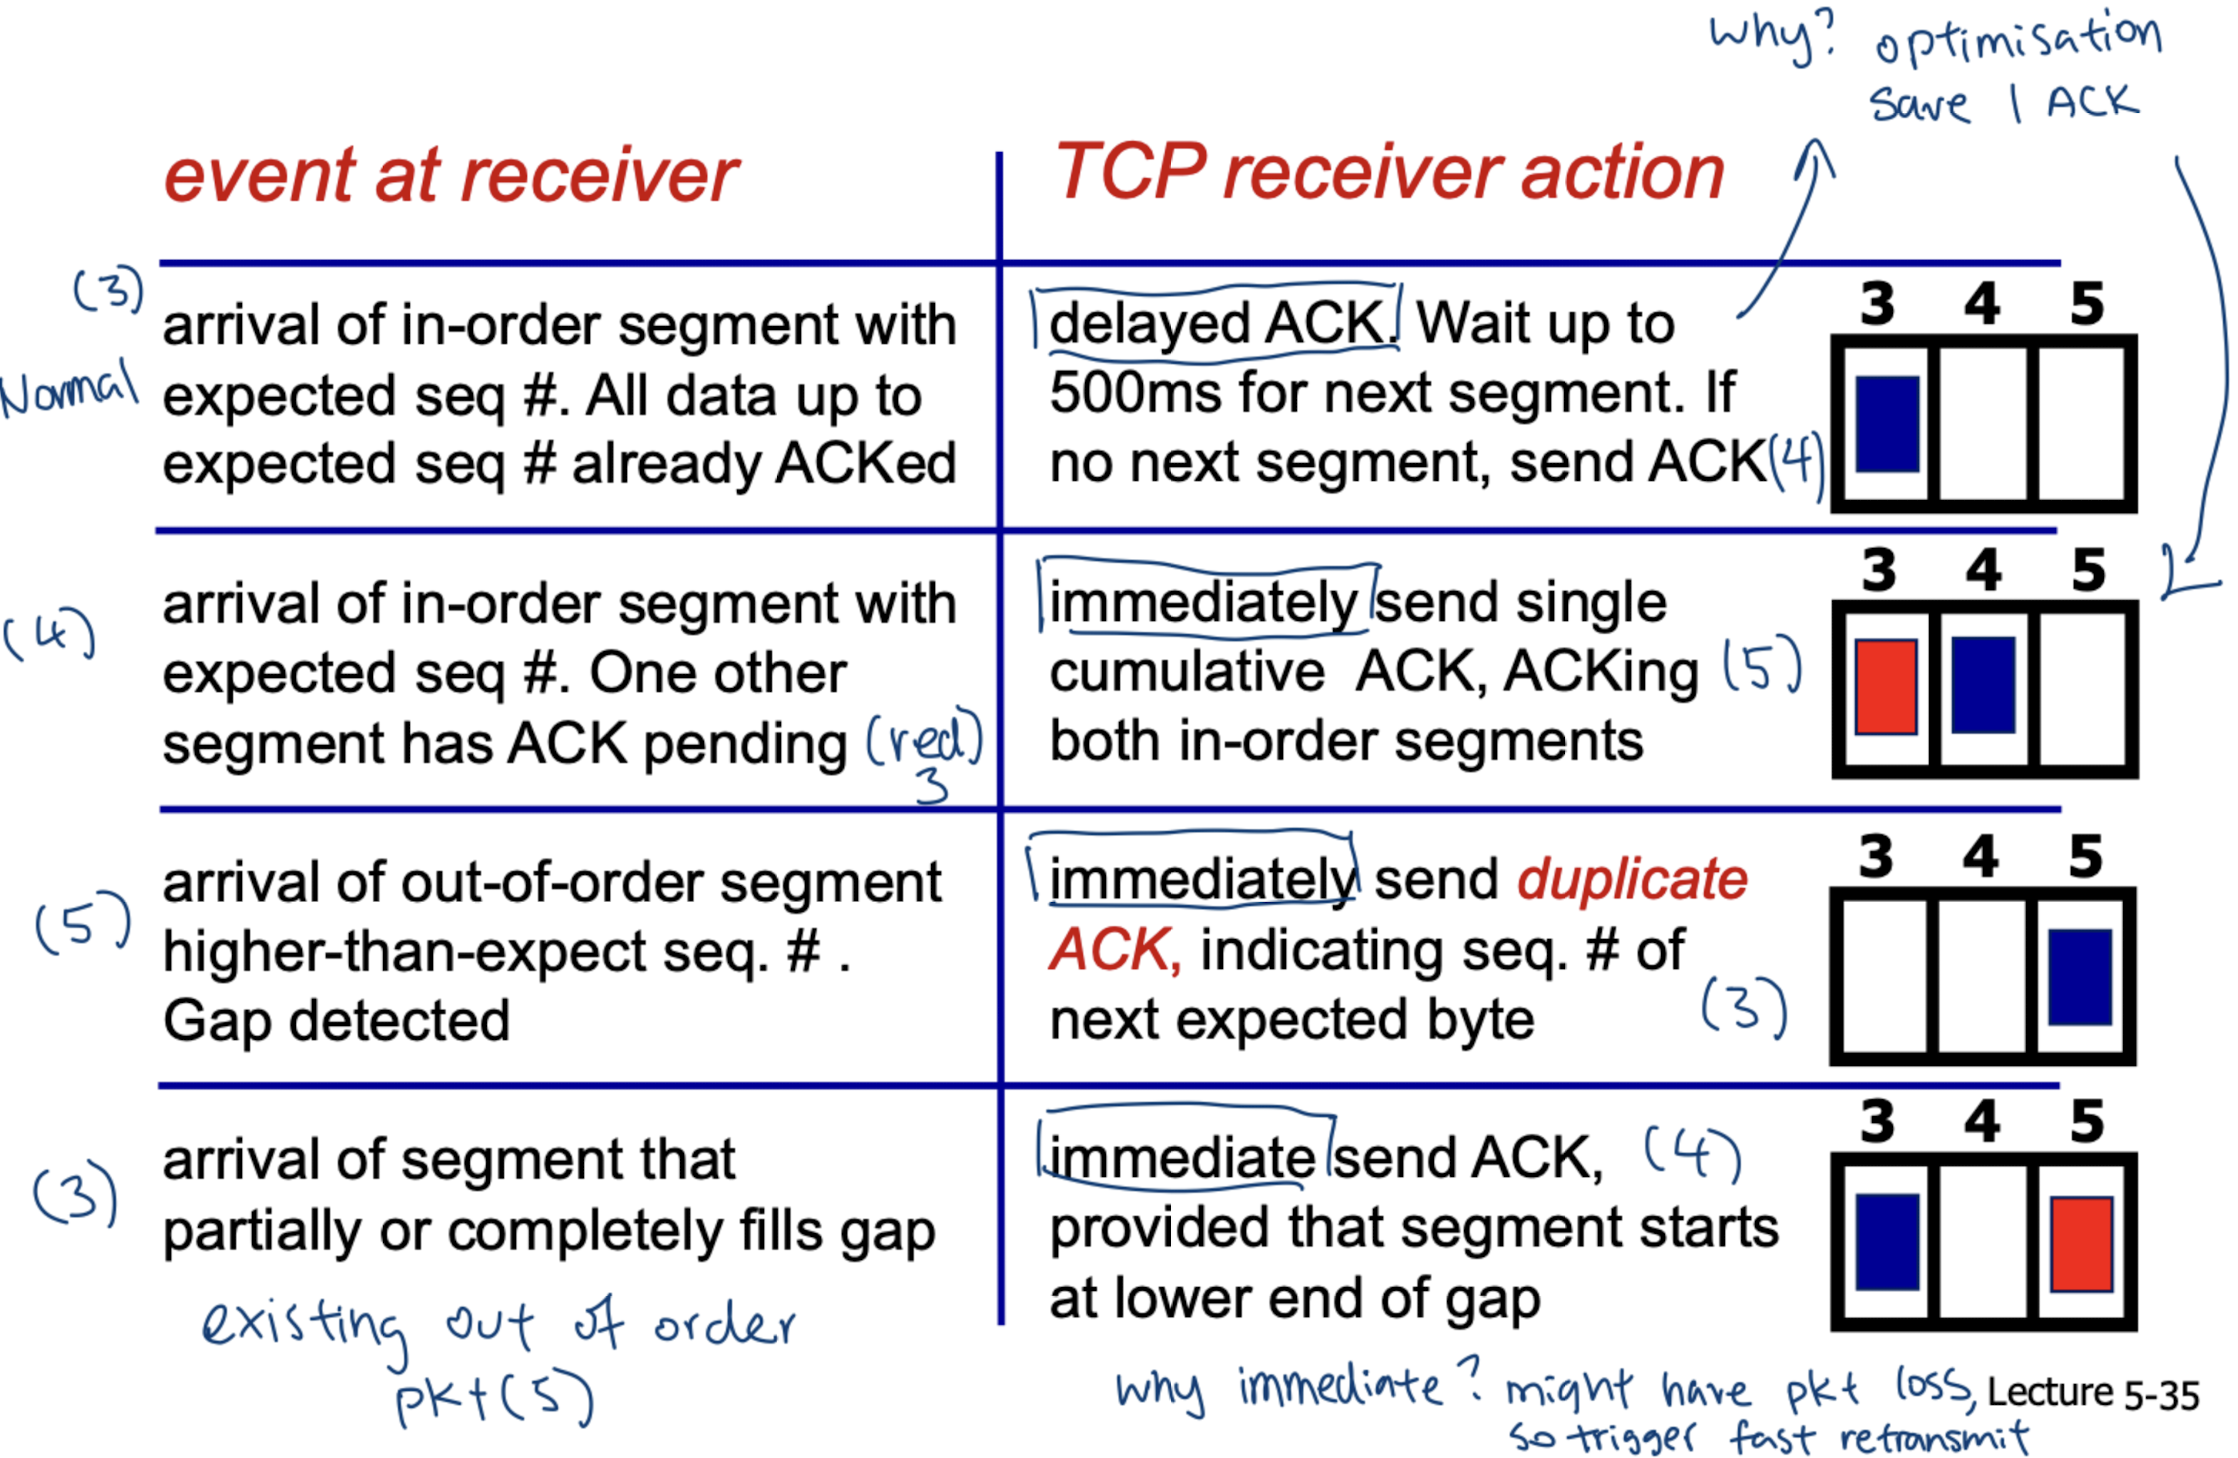
\includegraphics[scale=0.22]{tcp-receiver-event}

\begin{itemize}
    \item Delayed ACK for in-order segment
    \begin{itemize}
        \item If no next segment received in time, send ACK
        \item If next segment received in time, send ACK for 2nd segment (Saves 1 ACK. Works due to cumulative ACK.)
    \end{itemize}
    \item Immediate ACK for out-of-order segment (No matter if it creates or fills gap)
    \begin{itemize}
        \item Why immediate ACK? Might have packet loss, so can trigger fast retransmit earlier.
    \end{itemize}
\end{itemize}

\subsubsection{Timeout}

\begin{itemize}
    \item Motivation: What should timeout value be? Too short results in premature timeout. Too long results to slow reaction.
    \item \keyword{Sample RTT}{Measured time from segment transmission until ACK receipt. If retransmission, forget it.}
    \begin{itemize}
        \item Sample RTT varies a lot, so not accurate. How to get better estimate?
    \end{itemize}
    \item \keyword{Estimated RTT}{Average of recent measurements}
    \begin{itemize}
        \item Uses previous Estimated RTT
        \item Usually, $\alpha = 1/8$
    \end{itemize}
\end{itemize}

\[\text{Estimated RTT} = (1 - \alpha) * \text{Estimated RTT} + \alpha * \text{Sample RTT}\]

\begin{itemize}
    \item \keyword{Timeout Interval}{Estimated RTT + "Safety margin" (Deviation of estimate)}
    \begin{itemize}
        \item Usually, $\beta = 1/4$
    \end{itemize}
\end{itemize}

\[\text{Dev RTT} = (1 - \beta) * \text{Dev RTT} + \beta * | \text{Sample RTT} - \text{Estimated RTT} | \]

\[\text{Timeout Interval}  = \text{Estimated RTT} + 4 * \text{Dev RTT} \]

\subsubsection{Fast Retransmit}

\begin{itemize}
    \item Motivation: Timeout period often quite long. Long delay before resending lost pkt.
    \item \keyword{Fast Retransmit}{If sender receives 4 ACKs for same data, resend un-ACKed segment with smallest sequence number}
\end{itemize}

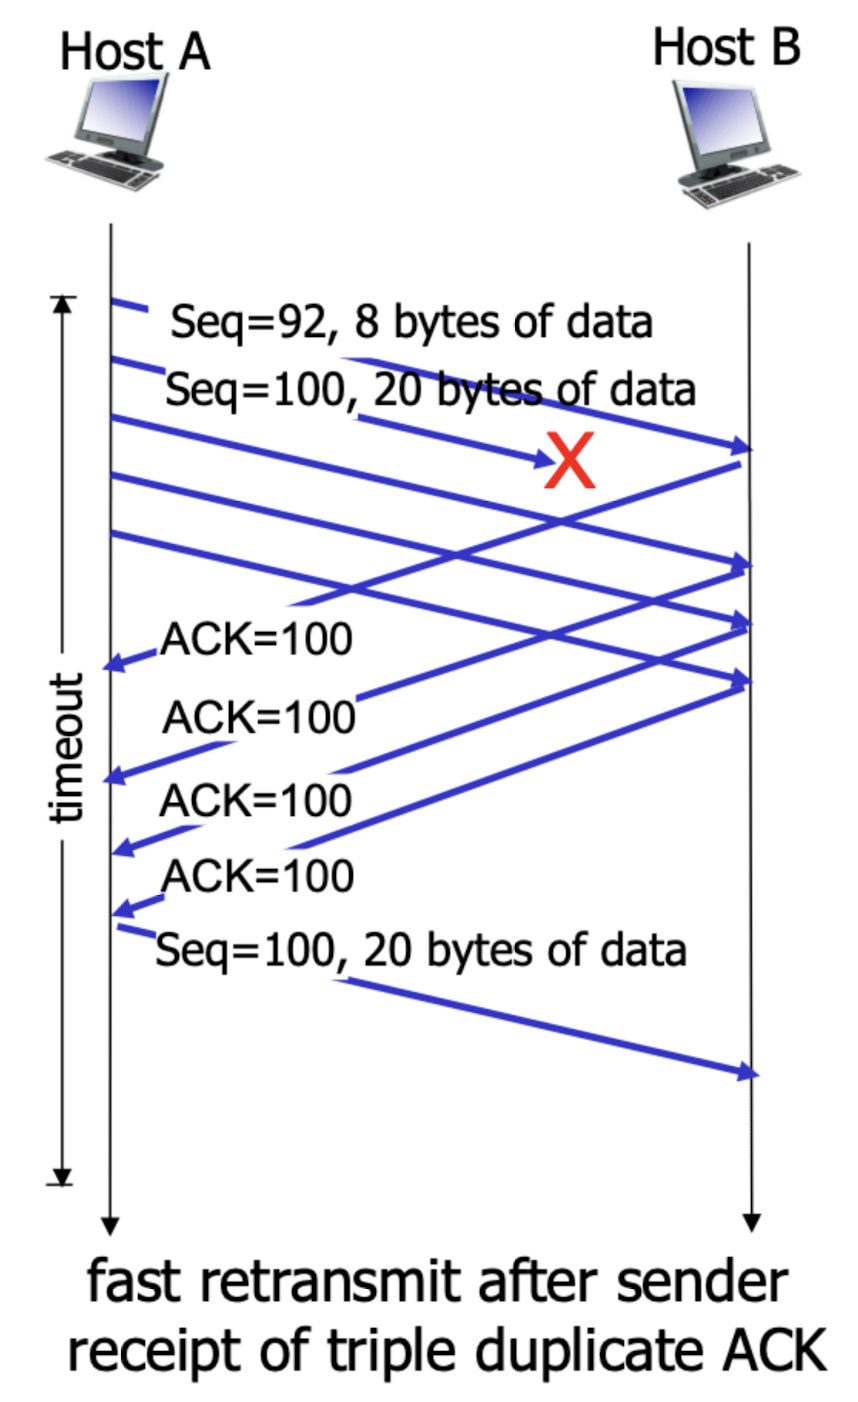
\includegraphics[scale=0.3]{tcp-fast-retransmit}

\section{06. IP Addressing}

\subsection{Network Layer}

\begin{itemize}
    \item Transports segments from sending to receiving \textbf{hosts}
    \item Network layer protocls in every host and router
    \item Key network functions:
    \begin{enumerate}
        \item \keyword{Forwarding}{Move packets from router's input to some router output}
        \item \keyword{Routing}{Determine route taken by packets from source to destination}
    \end{enumerate}
    \item \keyword{Data Plane}{Handles forwarding function}
    \begin{itemize}
        \item Local, per-router function
    \end{itemize}
    \item \keyword{Control Plane}{Handles routing function}
    \begin{itemize}
        \item Network-wide logic (since requires talking with other routers)
        \item 2 approaches: Traditional routing algorithms implemented in routers and software-defined networking implemented in servers
    \end{itemize}
\end{itemize}

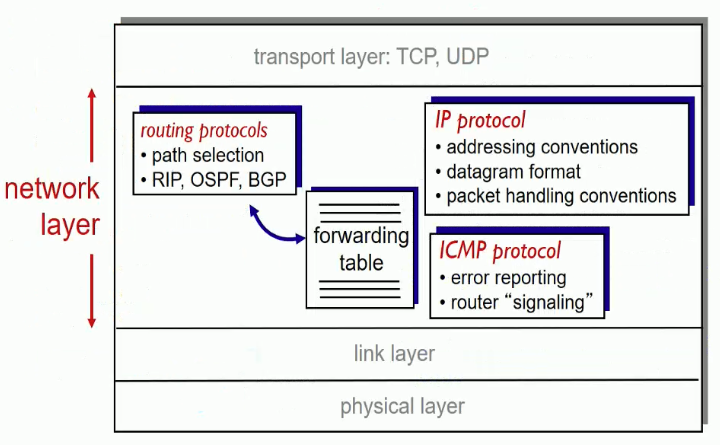
\includegraphics[scale=0.2]{network-layer}

\subsection{IP Protocol}

\begin{itemize}
    \item \keyword{IP Address}{32-bit identifier for host and router interface}
    \item \keyword{Interface}{Connection between host/router and physical link}
    \begin{itemize}
        \item Routers usually have many interfaces
        \item Hosts usually have 1-2 interfaces
        \item IP addresses associated with each interface
    \end{itemize}
\end{itemize}

\subsubsection{Subnet}

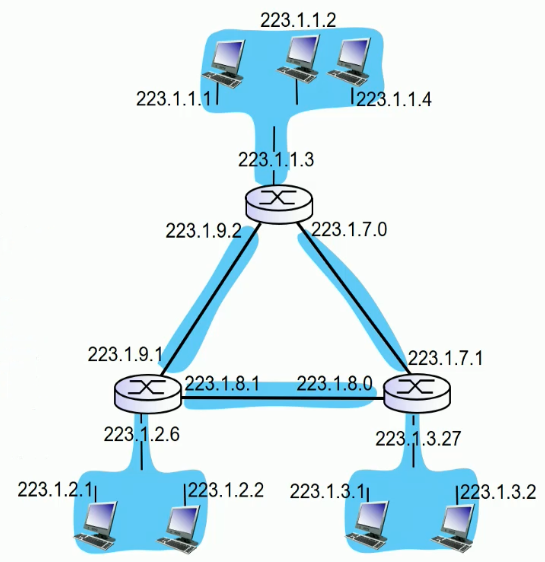
\includegraphics[scale=0.2]{subnets}

\begin{itemize}
    \item \keyword{Subnet}{Network formed by group of "directly" interconnected hosts (i.e. Can reach each other without router)}
    \begin{itemize}
        \item To find out how many: Remove routers and count number of isolated networks (Single links count)
        \item Hosts in same subnet have same network prefix of IP address
    \end{itemize}
\end{itemize}

\subsubsection{Classless InterDomain Routing (CIDR)}

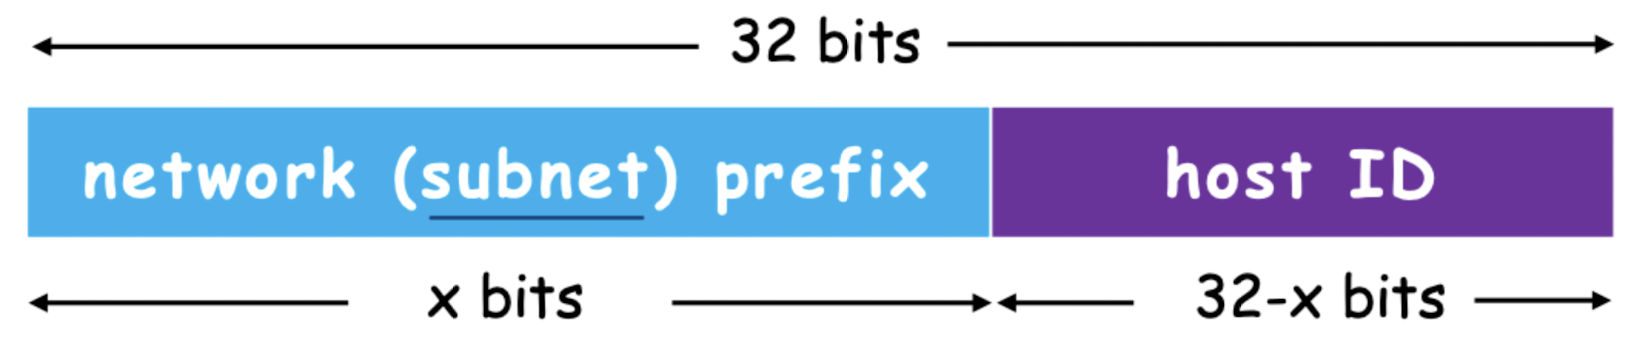
\includegraphics[scale=0.2]{cidr}

\begin{itemize}
    \item Some length for subnet portion
    \item Address format: $a.b.c.d/x$ where $x$ is number of bits in subnet portion
    \item \keyword{Subnet Mask}{Set all network prefix bits to $1$ and host ID bits to $0$}
    \begin{itemize}
        \item Used to determine which network an IP belongs to using bitwise AND
    \end{itemize}
\end{itemize}

\subsubsection{IP Address Allocation}

\begin{itemize}
    \item How do ISPs get blocks of addresses? Internet Corporation for Assigned Names and Numbers (ICANN), NPO that allocates addresses
\end{itemize}

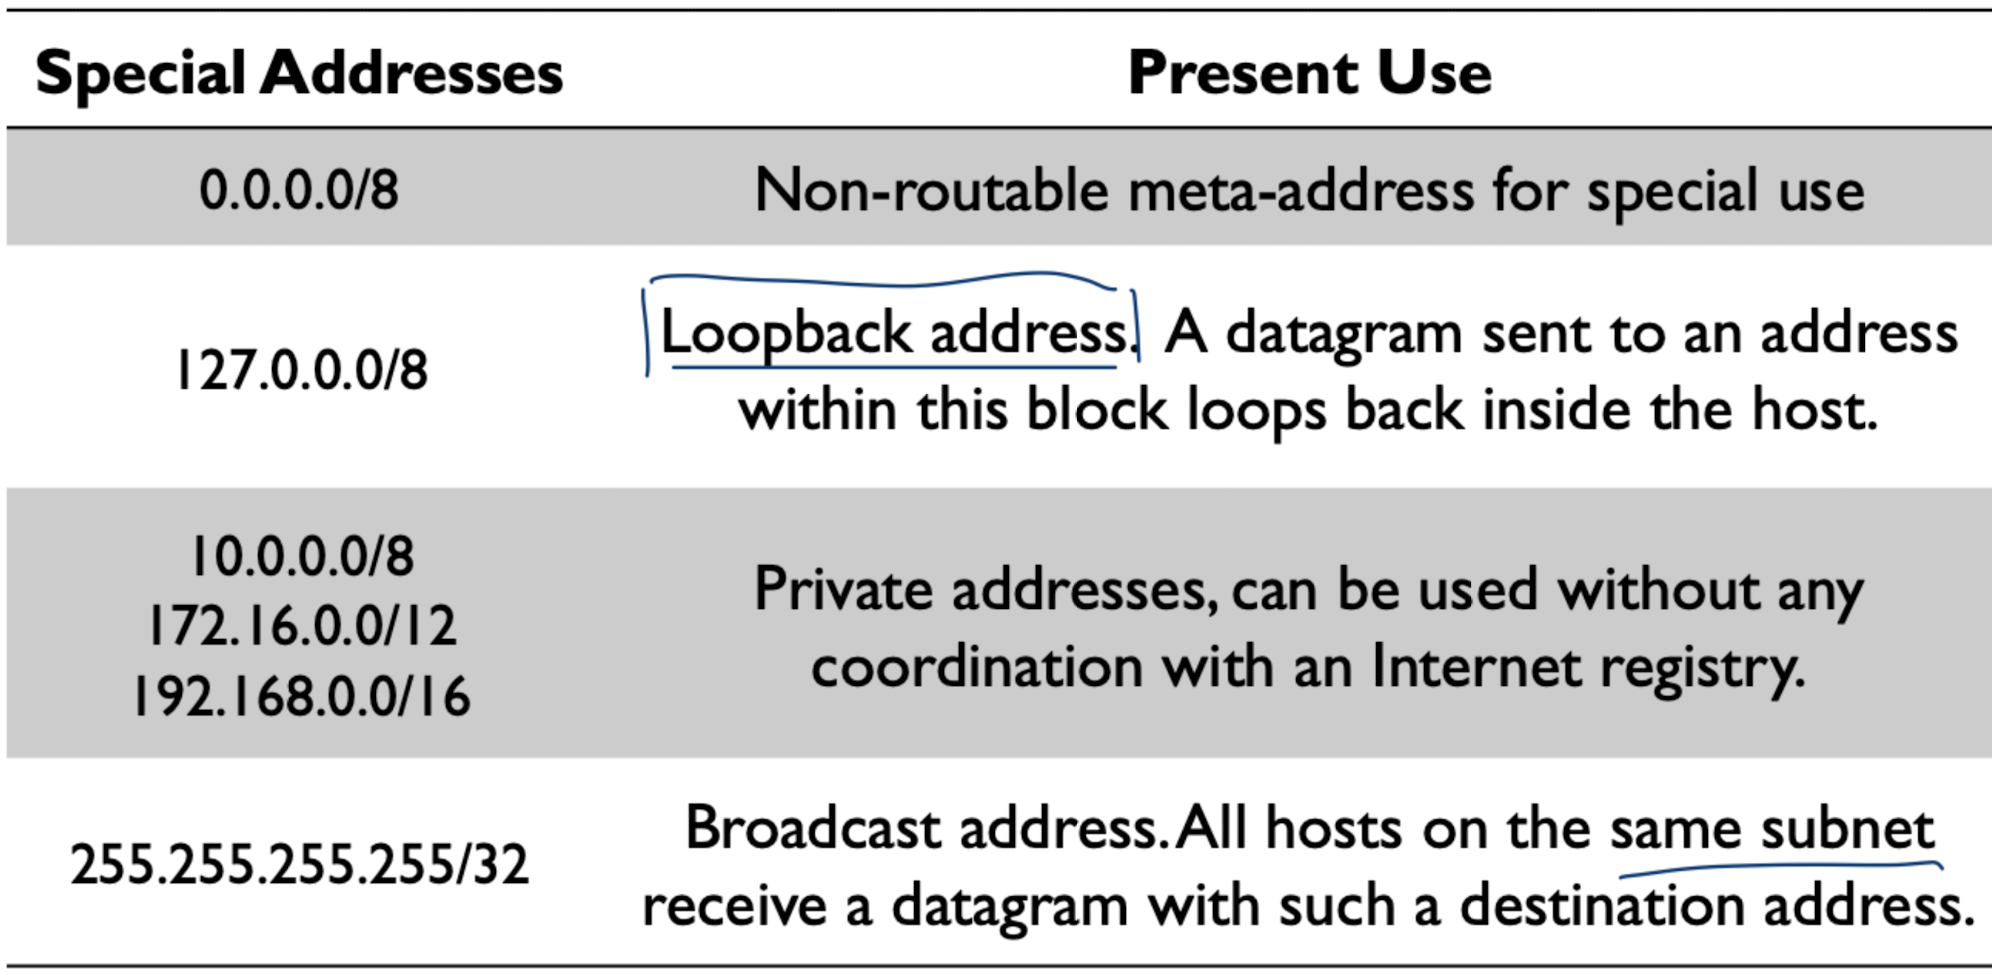
\includegraphics[scale=0.2]{special-ip-addresses}

\begin{itemize}
    \item How do organizations get block of address? Buy from registry or rent from ISP's address space
    \item Example of renting: 
    \begin{itemize}
        \item ISP's block: 200.23.16.0/20 (ISP can allocate to $2^{12}$ addresses)
        \item Use next 3 bits to differentiate $2^3 = 8$ organizations
        \item E.g. Org 0 takes 200.23.16.0/23, Org 1 takes 200.23.18.0/23
    \end{itemize}
\end{itemize}

\subsubsection{Hierarchical Addressing}

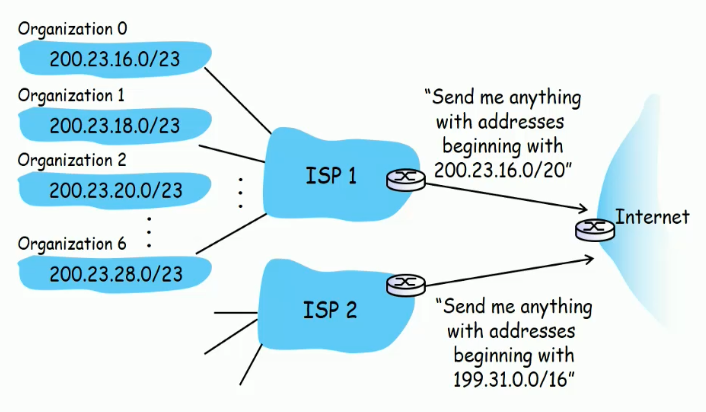
\includegraphics[scale=0.2]{hierarchical-addressing}

\begin{itemize}
    \item Allows efficient advertisement of routing information, rather than having mapping for $2^{32}$ addresses
    \item \keyword{Longest Prefix Matching}{How router decides address to deliver to}
\end{itemize}

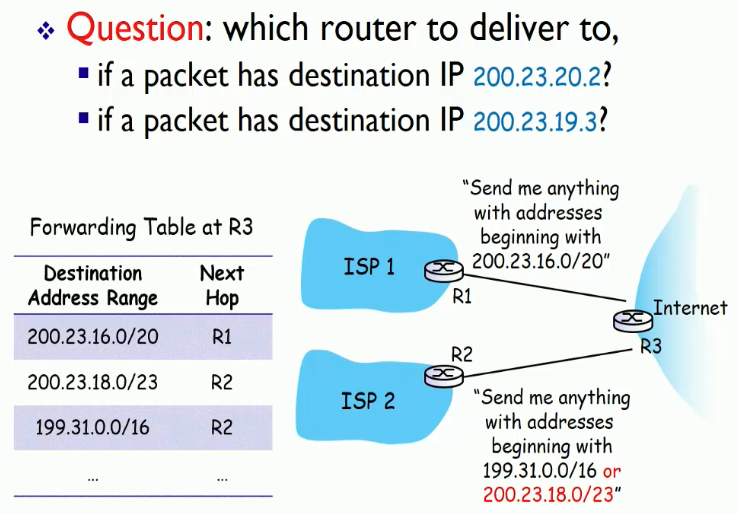
\includegraphics[scale=0.2]{longest-prefix-matching-1}

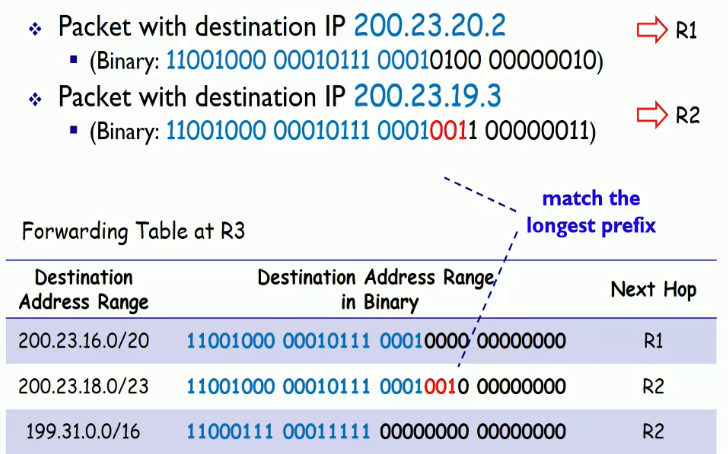
\includegraphics[scale=0.2]{longest-prefix-matching-2}

\subsubsection{How does a host get IP address?}

\begin{enumerate}
    \item Wired: Hard-coded by system admin
    \item Wireless: Dynamic Host Configuration Protocl (DHCP) dynamically gets address
\end{enumerate}

\subsubsection{Dynamic Host Configuration Protocl (DHCP)}

\begin{itemize}
    \item Goal: Allow host to dynamically get its IP address from network server upon joining
    \item Can also return address of first-hop router for client, name/IP address of DNS server, and network mask
    \item Runs over UDP (Server port: 67, Client port: 68)
    \item Subnets without DHCP server can rely on routers to relay from another subnet
    \item Process:
    \begin{enumerate}
        \item Optional: If host unsure what IP addresses are available, then host broadcasts "DHCP discover"
        \item Optional: Server responds with "DHCP offer"
        \item If host knows what IP address it wants, then host requests IP address (DHCP request)
        \item Server sends address (DHCP ack)
    \end{enumerate}
\end{itemize}

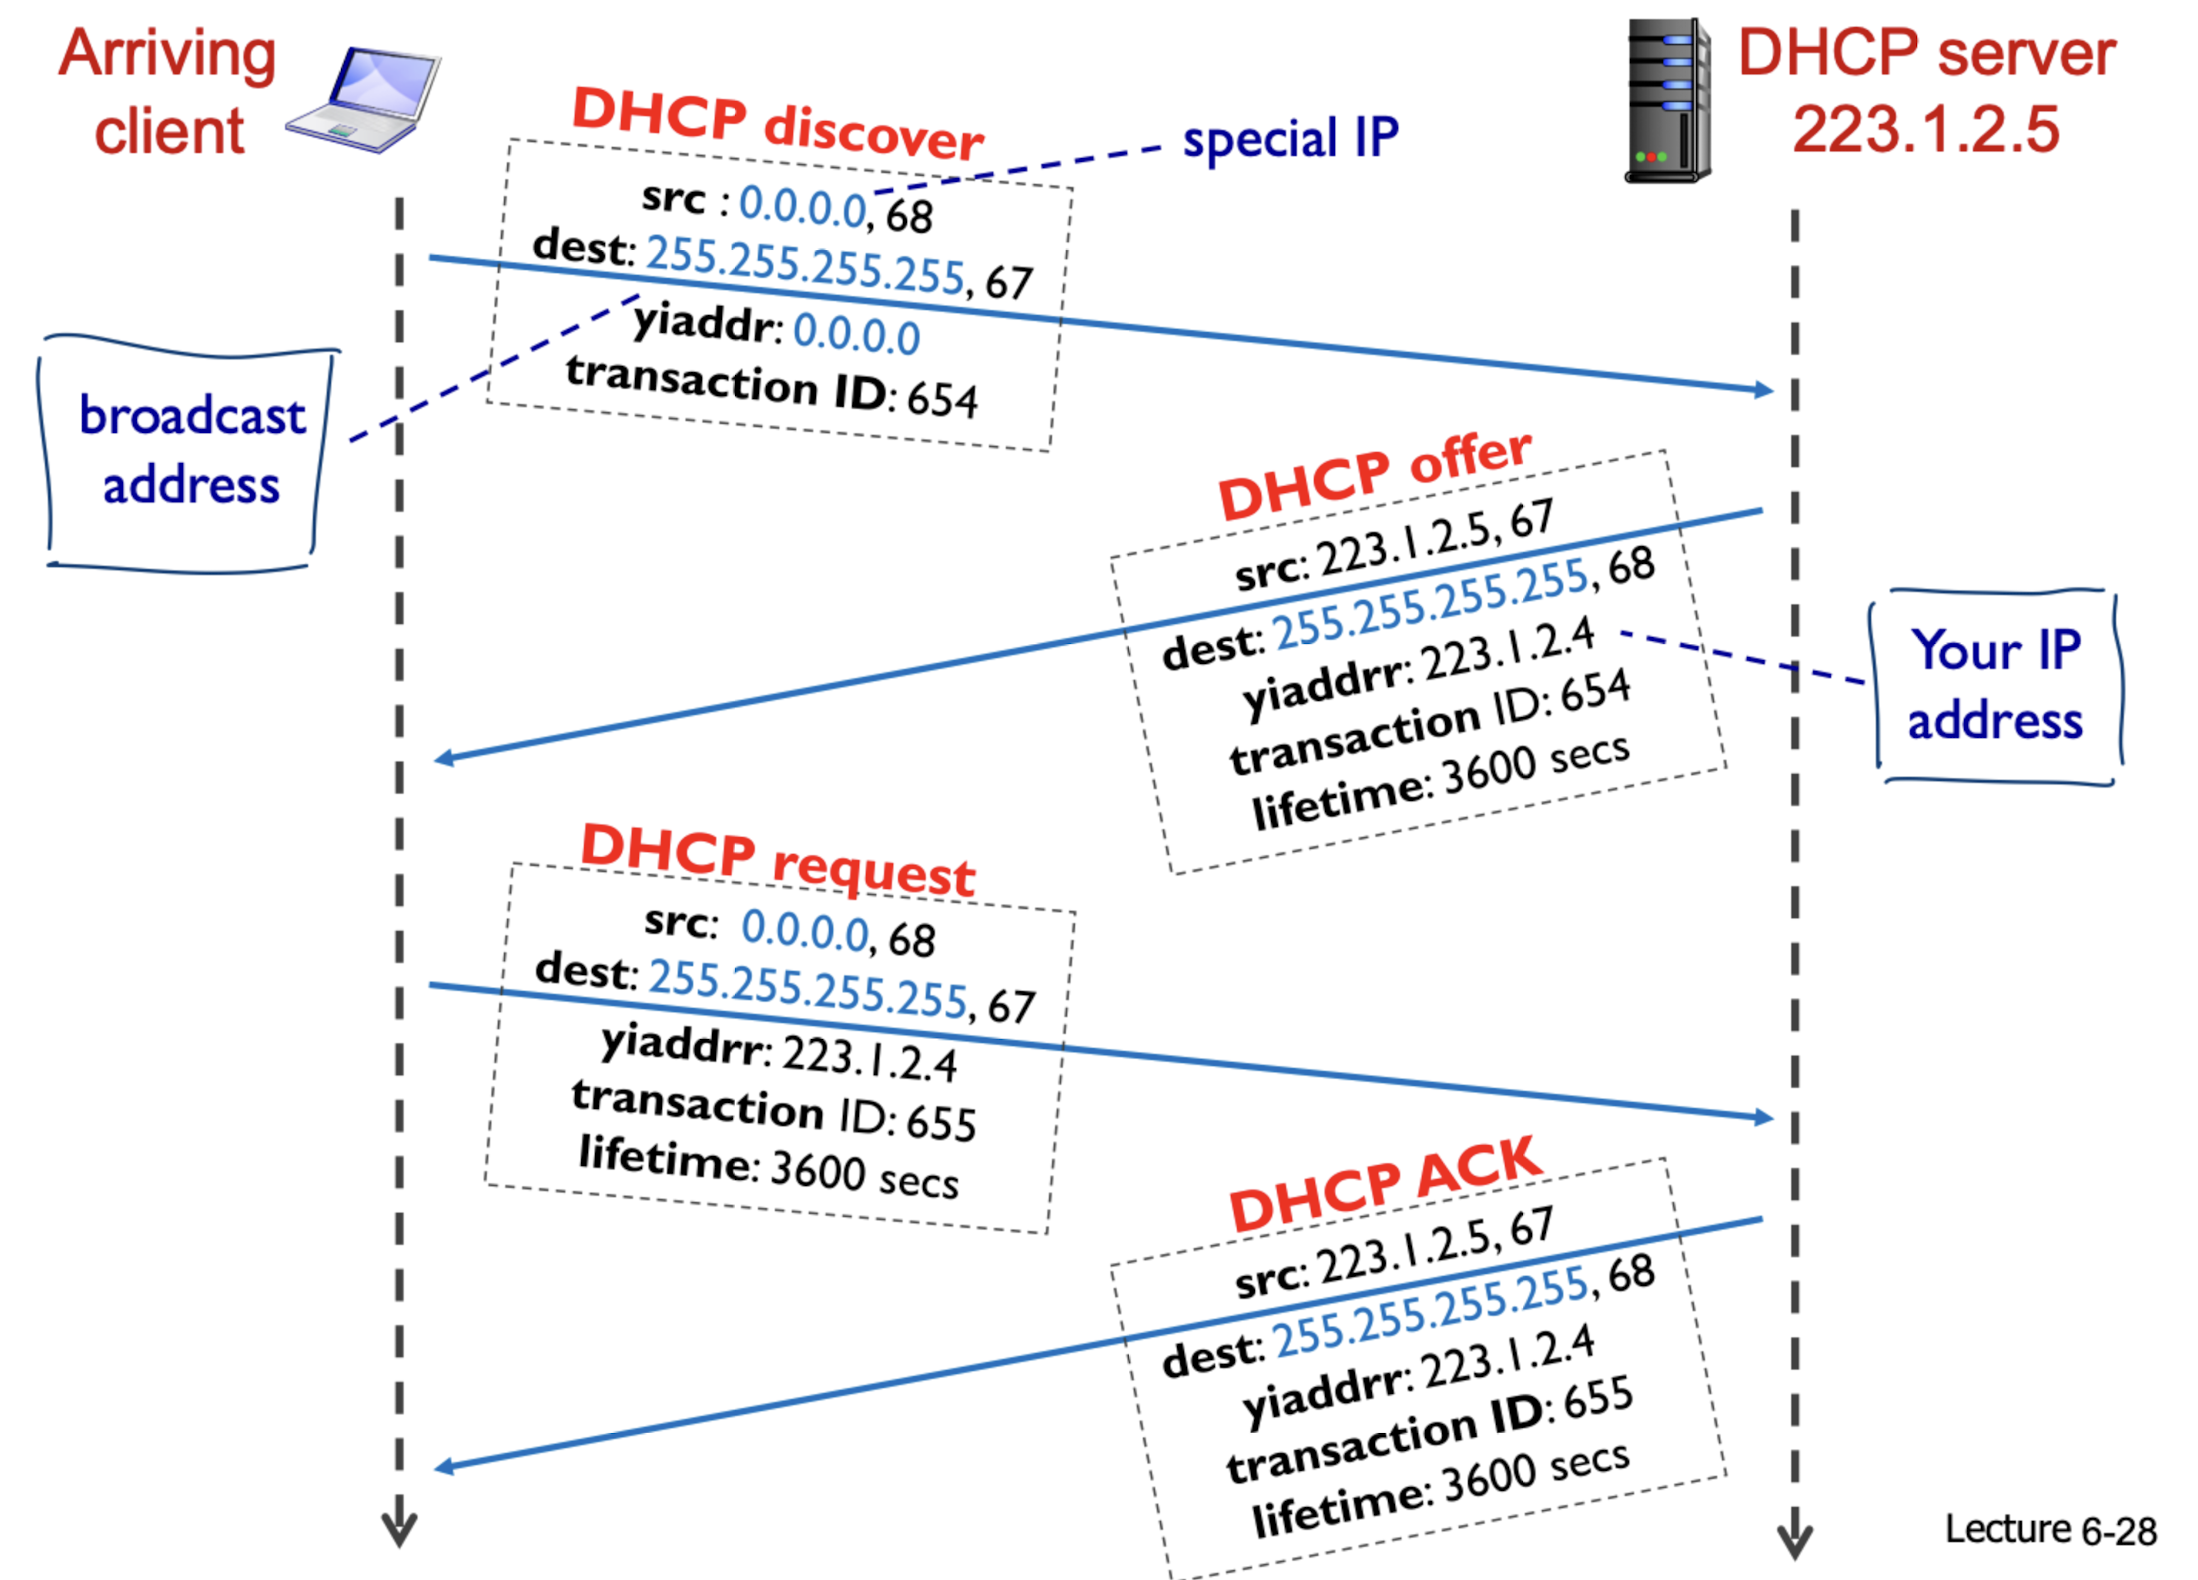
\includegraphics[scale=0.2]{dhcp}

\end{multicols*}
\end{document}
